\documentclass[8pt]{extarticle}
\usepackage[utf8]{inputenc}
\usepackage[T1]{fontenc}
\usepackage{amsmath, amssymb}
\usepackage{graphicx}
\usepackage{listings}
\usepackage{xcolor}
\usepackage[a4paper, landscape, left=1cm, right=1cm, top=1.5cm, bottom=1cm, headheight=15pt]{geometry}
\usepackage{multicol}
\usepackage{tocloft}
\usepackage[many]{tcolorbox}
\usepackage{needspace}
\usepackage{fancyhdr}
\pagestyle{fancy}
\fancyhf{}
\fancyhead[L]{\textbf{CSES Problem Set - UNICAMP}}
\fancyhead[R]{\textbf{Página \thepage}}
\renewcommand{\headrulewidth}{0.4pt}
\renewcommand{\footrulewidth}{0pt}
\fancypagestyle{plain}{
    \fancyhf{}
    \fancyhead[L]{\textbf{CSES Problem Set - UNICAMP}}
    \fancyhead[R]{\textbf{Página \thepage}}
    \renewcommand{\headrulewidth}{0.4pt}
}
\addtolength{\cftsecnumwidth}{0.5em}
\addtolength{\cftsubsecnumwidth}{1.2em}
\setlength{\columnseprule}{0.4pt}
\setlength{\columnsep}{25pt}

\newtcolorbox{caixaenunciado}{
    colback=gray!5,
    colframe=gray!40,
    arc=2pt,
    boxrule=0.5pt,
    left=4pt, right=4pt, top=4pt, bottom=4pt,
    breakable,
    lines before break=1,
    before skip=0.2cm, after skip=0.2cm
}

\lstset{
    language=C++,
    basicstyle=\ttfamily\footnotesize,
    keywordstyle=\color{blue},
    commentstyle=\color{green!50!black},
    stringstyle=\color{red},
    numbers=left,
    numberstyle=\tiny,
    numbersep=5pt,
    stepnumber=1,
    xleftmargin=2.0em,
    framexleftmargin=2.0em,
    breaklines=true,
    tabsize=4,
    extendedchars=true,
    literate={á}{{\'a}}1 {ã}{{\~a}}1 {é}{{\'e}}1 {í}{{\'i}}1 {ó}{{\'o}}1 {õ}{{\~o}}1 {ú}{{\'u}}1 {ç}{{\c{c}}}1 {Á}{{\'A}}1 {É}{{\'E}}1 {Í}{{\'I}}1 {Ó}{{\'O}}1 {Ú}{{\'U}}1 {Ç}{{\c{C}}}1 {Ã}{{\~A}}1 {Õ}{{\~O}}1
}

\usepackage[hidelinks]{hyperref}

\begin{document}
\raggedbottom
\begin{titlepage}
    \centering
    \vspace*{1.5cm}
    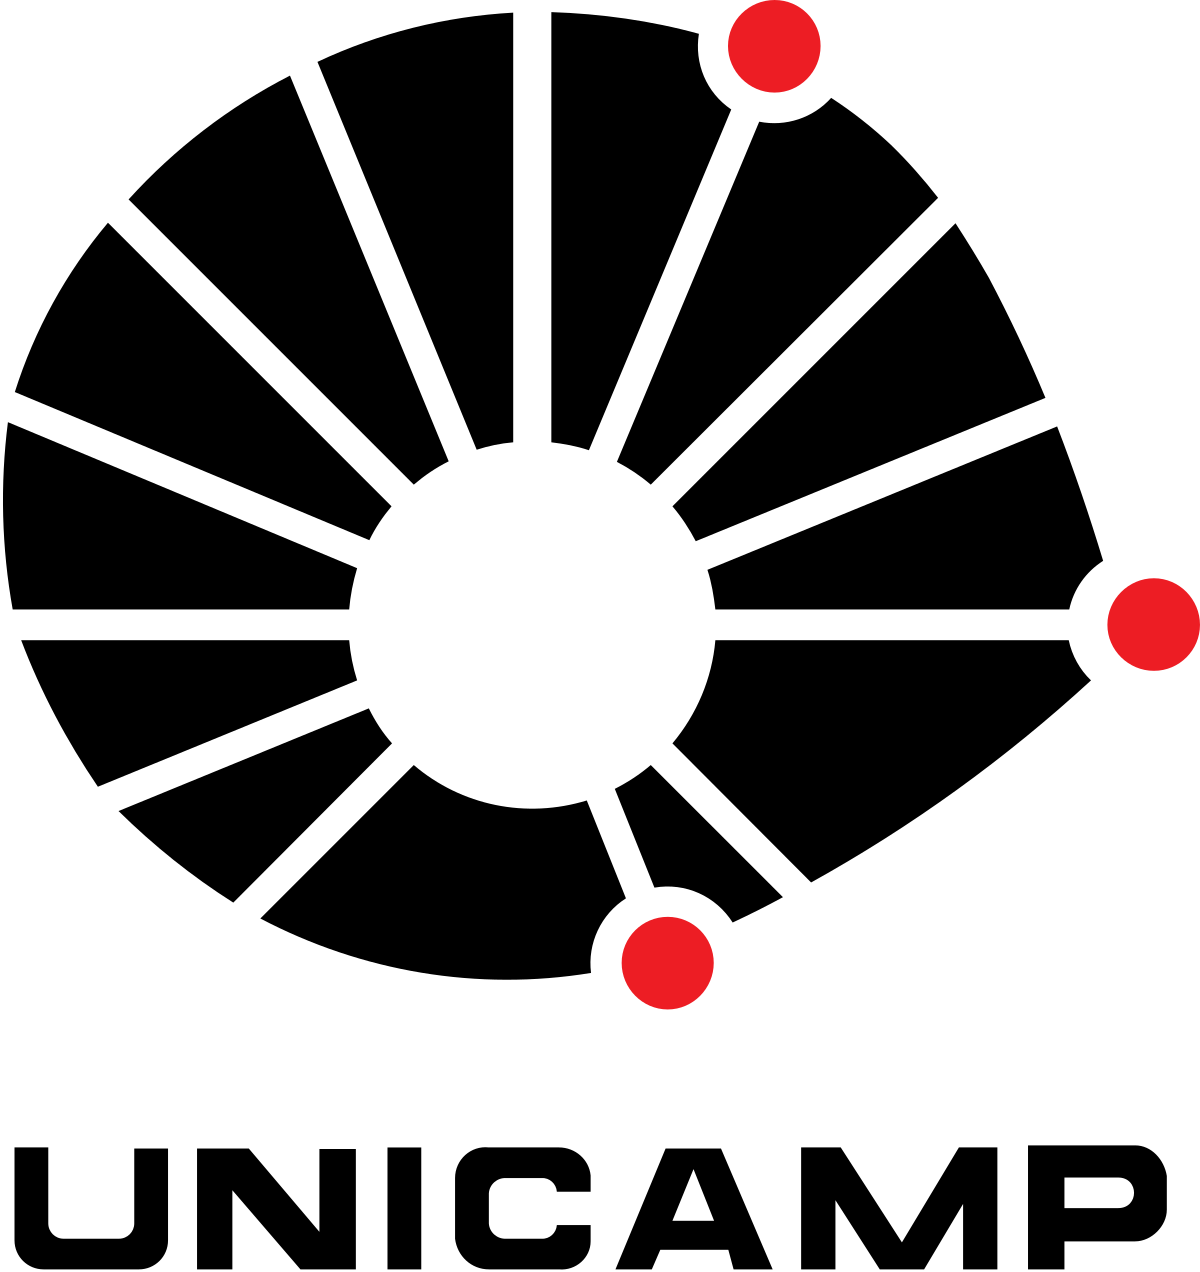
\includegraphics[width=4.5cm]{../assets/unicamp.png} \par
    \vspace{0.4cm}
    {\fontsize{16}{20}\selectfont Universidade Estadual de Campinas \par}
    \vspace{1.2cm}
    {\fontsize{42}{50}\selectfont Enemy Leo used Appeal! It's \par}
    \vspace{0.2cm}
    {\fontsize{42}{50}\selectfont super effective! Pikachu fainted! \par}
    \vspace{1.5cm}
    {\fontsize{20}{24}\selectfont \textbf{CSES Problem Set} \par}
    \vspace{1cm}
    {\fontsize{14}{18}\selectfont Pedro Assunção, Pedro Ferreira, Yvens Porto \par}
    \vfill
    {\fontsize{12}{14}\selectfont 2026-08-29 \par}
\end{titlepage}
\begin{multicols*}{3}
\tableofcontents
\end{multicols*}
\pagebreak
\begin{multicols*}{3}

\section{Introductory Problems}

\needspace{6\baselineskip}
\subsection{Apple Division}
\begin{caixaenunciado}
There are $n$ apples with known weights. Your task is to divide the apples into two groups so that the difference between the weights of the groups is minimal.

\vspace{0.3cm}\noindent\textbf{Input}

The first input line has an integer $n$: the number of apples.
The next line has $n$ integers $p_1,p_2,\dots,p_n$: the weight of each apple.

\vspace{0.3cm}\noindent\textbf{Output}

Print one integer: the minimum difference between the weights of the groups.

\vspace{0.3cm}\noindent\textbf{Constraints}

\textbullet\ $1 \le n \le 20$
\textbullet\ $1 \le p_i \le 10^9$
\end{caixaenunciado}
\vspace{0.3cm}
\lstinputlisting{src_limpo/IntroductoryProblems/AppleDivision.cpp}

\needspace{6\baselineskip}
\subsection{Bit Strings}
\begin{caixaenunciado}
Your task is to calculate the number of bit strings of length $n$.
For example, if $n=3$, the correct answer is $8$, because the possible bit strings are 000, 001, 010, 011, 100, 101, 110, and 111.

\vspace{0.3cm}\noindent\textbf{Input}

The only input line has an integer $n$.

\vspace{0.3cm}\noindent\textbf{Output}

Print the result modulo $10^9+7$.

\vspace{0.3cm}\noindent\textbf{Constraints}

\textbullet\ $1 \le n \le 10^6$
\end{caixaenunciado}
\vspace{0.3cm}
\lstinputlisting{src_limpo/IntroductoryProblems/BitStrings.cpp}

\needspace{6\baselineskip}
\subsection{Chessboard And Queens}
\begin{caixaenunciado}
\input{../enunciados/IntroductoryProblems/ChessboardAndQueens.tex}
\end{caixaenunciado}
\vspace{0.3cm}
\lstinputlisting{src_limpo/IntroductoryProblems/ChessboardAndQueens.cpp}

\needspace{6\baselineskip}
\subsection{Coin Piles}
\begin{caixaenunciado}
You have two coin piles containing $a$ and $b$ coins. On each move, you can either remove one coin from the left pile and two coins from the right pile, or two coins from the left pile and one coin from the right pile.
Your task is to efficiently find out if you can empty both the piles.

\vspace{0.3cm}\noindent\textbf{Input}

The first input line has an integer $t$: the number of tests.
After this, there are $t$ lines, each of which has two integers $a$ and $b$: the numbers of coins in the piles.

\vspace{0.3cm}\noindent\textbf{Output}

For each test, print "YES" if you can empty the piles and "NO" otherwise.

\vspace{0.3cm}\noindent\textbf{Constraints}

\textbullet\ $1 \le t \le 10^5$
\textbullet\ $0 \le a, b \le 10^9$
\end{caixaenunciado}
\vspace{0.3cm}
\lstinputlisting{src_limpo/IntroductoryProblems/CoinPiles.cpp}

\needspace{6\baselineskip}
\subsection{Creating Strings}
\begin{caixaenunciado}
Given a string, your task is to generate all different strings that can be created using its characters.

\vspace{0.3cm}\noindent\textbf{Input}

The only input line has a string of length $n$. Each character is between a–z.

\vspace{0.3cm}\noindent\textbf{Output}

First print an integer $k$: the number of strings. Then print $k$ lines: the strings in alphabetical order.

\vspace{0.3cm}\noindent\textbf{Constraints}

\textbullet\ $1 \le n \le 8$
\end{caixaenunciado}
\vspace{0.3cm}
\lstinputlisting{src_limpo/IntroductoryProblems/CreatingStrings.cpp}

\needspace{6\baselineskip}
\subsection{Digit Queries}
\begin{caixaenunciado}
Consider an infinite string that consists of all positive integers in increasing order:
12345678910111213141516171819202122232425...
Your task is to process $q$ queries of the form: what is the digit at position $k$ in the string?

\vspace{0.3cm}\noindent\textbf{Input}

The first input line has an integer $q$: the number of queries.
After this, there are $q$ lines that describe the queries. Each line has an integer $k$: a $1$-indexed position in the string.

\vspace{0.3cm}\noindent\textbf{Output}

For each query, print the corresponding digit.

\vspace{0.3cm}\noindent\textbf{Constraints}

\textbullet\ $1 \le q \le 1000$
\textbullet\ $1 \le k \le 10^{18}$
\end{caixaenunciado}
\vspace{0.3cm}
\lstinputlisting{src_limpo/IntroductoryProblems/DigitQueries.cpp}

\needspace{6\baselineskip}
\subsection{Gray Code}
\begin{caixaenunciado}
A Gray code is a list of all $2^n$ bit strings of length $n$, where any two successive strings differ in exactly one bit (i.e., their Hamming distance is one).
Your task is to create a Gray code for a given length $n$.

\vspace{0.3cm}\noindent\textbf{Input}

The only input line has an integer $n$.

\vspace{0.3cm}\noindent\textbf{Output}

Print $2^n$ lines that describe the Gray code. You can print any valid solution.

\vspace{0.3cm}\noindent\textbf{Constraints}

\textbullet\ $1 \le n \le 16$
\end{caixaenunciado}
\vspace{0.3cm}
\lstinputlisting{src_limpo/IntroductoryProblems/GrayCode.cpp}

\needspace{6\baselineskip}
\subsection{Grid Coloring I}
\begin{caixaenunciado}
\input{../enunciados/IntroductoryProblems/GridColoringI.tex}
\end{caixaenunciado}
\vspace{0.3cm}
\lstinputlisting{src_limpo/IntroductoryProblems/GridColoringI.cpp}

\needspace{6\baselineskip}
\subsection{Grid Path Description}
\begin{caixaenunciado}
\input{../enunciados/IntroductoryProblems/GridPathDescription.tex}
\end{caixaenunciado}
\vspace{0.3cm}
\lstinputlisting{src_limpo/IntroductoryProblems/GridPathDescription.cpp}

\needspace{6\baselineskip}
\subsection{Increasing Array}
\begin{caixaenunciado}
You are given an array of $n$ integers. You want to modify the array so that it is increasing, i.e., every element is at least as large as the previous element.
On each move, you may increase the value of any element by one. What is the minimum number of moves required?

\vspace{0.3cm}\noindent\textbf{Input}

The first input line contains an integer $n$: the size of the array.
Then, the second line contains $n$ integers $x_1,x_2,\ldots,x_n$: the contents of the array.

\vspace{0.3cm}\noindent\textbf{Output}

Print the minimum number of moves.

\vspace{0.3cm}\noindent\textbf{Constraints}

\textbullet\ $1 \le n \le 2 \cdot 10^5$
\textbullet\ $1 \le x_i \le 10^9$
\end{caixaenunciado}
\vspace{0.3cm}
\lstinputlisting{src_limpo/IntroductoryProblems/IncreasingArray.cpp}

\needspace{6\baselineskip}
\subsection{Knight Moves Grid}
\begin{caixaenunciado}
There is a knight on an $n \times n$ chessboard. For each square, print the minimum number of moves the knight needs to do to reach the top-left corner.

\vspace{0.3cm}\noindent\textbf{Input}

The only line has an integer $n$.

\vspace{0.3cm}\noindent\textbf{Output}

Print the number of moves for each square.

\vspace{0.3cm}\noindent\textbf{Constraints}

\textbullet\ $4 \le n \le 1000$
\end{caixaenunciado}
\vspace{0.3cm}
\lstinputlisting{src_limpo/IntroductoryProblems/KnightMovesGrid.cpp}

\needspace{6\baselineskip}
\subsection{Mex Grid Construction}
\begin{caixaenunciado}
Your task is to construct an $n \times n$ grid where each square has the smallest nonnegative integer that does not appear to the left on the same row or above on the same column.

\vspace{0.3cm}\noindent\textbf{Input}

The only line has an integer $n$.

\vspace{0.3cm}\noindent\textbf{Output}

Print the grid according to the example.

\vspace{0.3cm}\noindent\textbf{Constraints}

\textbullet\ $1 \le n \le 100$
\end{caixaenunciado}
\vspace{0.3cm}
\lstinputlisting{src_limpo/IntroductoryProblems/MexGridConstruction.cpp}

\needspace{6\baselineskip}
\subsection{Missing Number}
\begin{caixaenunciado}
You are given all numbers between $1,2,\ldots,n$ except one. Your task is to find the missing number.

\vspace{0.3cm}\noindent\textbf{Input}

The first input line contains an integer $n$.
The second line contains $n-1$ numbers. Each number is distinct and between $1$ and $n$ (inclusive).

\vspace{0.3cm}\noindent\textbf{Output}

Print the missing number.

\vspace{0.3cm}\noindent\textbf{Constraints}

\textbullet\ $2 \le n \le 2 \cdot 10^5$
\end{caixaenunciado}
\vspace{0.3cm}
\lstinputlisting{src_limpo/IntroductoryProblems/MissingNumber.cpp}

\needspace{6\baselineskip}
\subsection{Number Spiral}
\begin{caixaenunciado}
A number spiral is an infinite grid whose upper-left square has number 1. Here are the first five layers of the spiral:

Your task is to find out the number in row $y$ and column $x$.

\vspace{0.3cm}\noindent\textbf{Input}

The first input line contains an integer $t$: the number of tests.
After this, there are $t$ lines, each containing integers $y$ and $x$.

\vspace{0.3cm}\noindent\textbf{Output}

For each test, print the number in row $y$ and column $x$.

\vspace{0.3cm}\noindent\textbf{Constraints}

\textbullet\ $1 \le t \le 10^5$
\textbullet\ $1 \le y,x \le 10^9$
\end{caixaenunciado}
\vspace{0.3cm}
\lstinputlisting{src_limpo/IntroductoryProblems/NumberSpiral.cpp}

\needspace{6\baselineskip}
\subsection{Palindrome Reorder}
\begin{caixaenunciado}
Given a string, your task is to reorder its letters in such a way that it becomes a palindrome (i.e., it reads the same forwards and backwards).

\vspace{0.3cm}\noindent\textbf{Input}

The only input line has a string of length $n$ consisting of characters A–Z.

\vspace{0.3cm}\noindent\textbf{Output}

Print a palindrome consisting of the characters of the original string. You may print any valid solution. If there are no solutions, print "NO SOLUTION".

\vspace{0.3cm}\noindent\textbf{Constraints}

\textbullet\ $1 \le n \le 10^6$
\end{caixaenunciado}
\vspace{0.3cm}
\lstinputlisting{src_limpo/IntroductoryProblems/PalindromeReorder.cpp}

\needspace{6\baselineskip}
\subsection{Permutations}
\begin{caixaenunciado}
A permutation of integers $1,2,\ldots,n$ is called beautiful if there are no adjacent elements whose difference is $1$.
Given $n$, construct a beautiful permutation if such a permutation exists.

\vspace{0.3cm}\noindent\textbf{Input}

The only input line contains an integer $n$.

\vspace{0.3cm}\noindent\textbf{Output}

Print a beautiful permutation of integers $1,2,\ldots,n$. If there are several solutions, you may print any of them. If there are no solutions, print "NO SOLUTION".

\vspace{0.3cm}\noindent\textbf{Constraints}

\textbullet\ $1 \le n \le 10^6$
\end{caixaenunciado}
\vspace{0.3cm}
\lstinputlisting{src_limpo/IntroductoryProblems/Permutations.cpp}

\needspace{6\baselineskip}
\subsection{Raab Game I}
\begin{caixaenunciado}
Consider a two player game where each player has $n$ cards numbered $1,2,\dots,n$. On each turn both players place one of their cards on the table. The player who placed the higher card gets one point. If the cards are equal, neither player gets a point. The game continues until all cards have been played.
You are given the number of cards $n$ and the players' scores at the end of the game, $a$ and $b$. Your task is to give an example of how the game could have played out.

\vspace{0.3cm}\noindent\textbf{Input}

The first line contains one integer $t$: the number of tests.
Then there are $t$ lines, each with three integers $n$, $a$ and $b$.

\vspace{0.3cm}\noindent\textbf{Output}

For each test case print YES if there is a game with the given outcome and NO otherwise.
If the answer is YES, print an example of one possible game. Print two lines representing the order in which the players place their cards. You can give any valid example.

\vspace{0.3cm}\noindent\textbf{Constraints}

\textbullet\ $1 \le t \le 1000$
\textbullet\ $1 \le n \le 100$
\textbullet\ $0 \le a,b \le n$
\end{caixaenunciado}
\vspace{0.3cm}
\lstinputlisting{src_limpo/IntroductoryProblems/RaabGameI.cpp}

\needspace{6\baselineskip}
\subsection{Repetitions}
\begin{caixaenunciado}
\input{../enunciados/IntroductoryProblems/Repetitions.tex}
\end{caixaenunciado}
\vspace{0.3cm}
\lstinputlisting{src_limpo/IntroductoryProblems/Repetitions.cpp}

\needspace{6\baselineskip}
\subsection{String Reorder}
\begin{caixaenunciado}
Your task is to reorder the characters of a string so that no two adjacent characters are the same. What is the lexicographically minimal such string?

\vspace{0.3cm}\noindent\textbf{Input}

The only line has a string of length $n$ consisting of characters A–Z.

\vspace{0.3cm}\noindent\textbf{Output}

Print the lexicographically minimal reordered string where no two adjacent characters are the same. If it is not possible to create such a string, print $-1$.

\vspace{0.3cm}\noindent\textbf{Constraints}

\textbullet\ $1 \le n \le 10^6$
\end{caixaenunciado}
\vspace{0.3cm}
\lstinputlisting{src_limpo/IntroductoryProblems/StringReorder.cpp}

\needspace{6\baselineskip}
\subsection{Tower Of Hanoi}
\begin{caixaenunciado}
\input{../enunciados/IntroductoryProblems/TowerOfHanoi.tex}
\end{caixaenunciado}
\vspace{0.3cm}
\lstinputlisting{src_limpo/IntroductoryProblems/TowerOfHanoi.cpp}

\needspace{6\baselineskip}
\subsection{Trailing Zeros}
\begin{caixaenunciado}
Your task is to calculate the number of trailing zeros in the factorial $n!$.
For example, $20!=2432902008176640000$ and it has $4$ trailing zeros.

\vspace{0.3cm}\noindent\textbf{Input}

The only input line has an integer $n$.

\vspace{0.3cm}\noindent\textbf{Output}

Print the number of trailing zeros in $n!$.

\vspace{0.3cm}\noindent\textbf{Constraints}

\textbullet\ $1 \le n \le 10^9$
\end{caixaenunciado}
\vspace{0.3cm}
\lstinputlisting{src_limpo/IntroductoryProblems/TrailingZeros.cpp}

\needspace{6\baselineskip}
\subsection{Two Knights}
\begin{caixaenunciado}
Your task is to count for $k=1,2,\ldots,n$ the number of ways two knights can be placed on a $k \times k$ chessboard so that they do not attack each other.

\vspace{0.3cm}\noindent\textbf{Input}

The only input line contains an integer $n$.

\vspace{0.3cm}\noindent\textbf{Output}

Print $n$ integers: the results.

\vspace{0.3cm}\noindent\textbf{Constraints}

\textbullet\ $1 \le n \le 10000$
\end{caixaenunciado}
\vspace{0.3cm}
\lstinputlisting{src_limpo/IntroductoryProblems/TwoKnights.cpp}

\needspace{6\baselineskip}
\subsection{Two Sets}
\begin{caixaenunciado}
Your task is to divide the numbers $1,2,\ldots,n$ into two sets of equal sum.

\vspace{0.3cm}\noindent\textbf{Input}

The only input line contains an integer $n$.

\vspace{0.3cm}\noindent\textbf{Output}

Print "YES", if the division is possible, and "NO" otherwise.
After this, if the division is possible, print an example of how to create the sets. First, print the number of elements in the first set followed by the elements themselves in a separate line, and then, print the second set in a similar way.

\vspace{0.3cm}\noindent\textbf{Constraints}

\textbullet\ $1 \le n \le 10^6$
\end{caixaenunciado}
\vspace{0.3cm}
\lstinputlisting{src_limpo/IntroductoryProblems/TwoSets.cpp}

\needspace{6\baselineskip}
\subsection{Weird Algorithm}
\begin{caixaenunciado}
Consider an algorithm that takes as input a positive integer $n$. If $n$ is even, the algorithm divides it by two, and if $n$ is odd, the algorithm multiplies it by three and adds one. The algorithm repeats this, until $n$ is one. For example, the sequence for $n=3$ is as follows:
$ 3 \rightarrow 10 \rightarrow 5 \rightarrow 16 \rightarrow 8 \rightarrow 4 \rightarrow 2 \rightarrow 1$
Your task is to simulate the execution of the algorithm for a given value of $n$.

\vspace{0.3cm}\noindent\textbf{Input}

The only input line contains an integer $n$.

\vspace{0.3cm}\noindent\textbf{Output}

Print a line that contains all values of $n$ during the algorithm.

\vspace{0.3cm}\noindent\textbf{Constraints}

\textbullet\ $1 \le n \le 10^6$
\end{caixaenunciado}
\vspace{0.3cm}
\lstinputlisting{src_limpo/IntroductoryProblems/WeirdAlgorithm.cpp}
\end{multicols*}
\pagebreak
\begin{multicols*}{3}

\section{Sorting And Searching}

\needspace{6\baselineskip}
\subsection{Apartments}
\begin{caixaenunciado}
There are $n$ applicants and $m$ free apartments. Your task is to distribute the apartments so that as many applicants as possible will get an apartment.
Each applicant has a desired apartment size, and they will accept any apartment whose size is close enough to the desired size.

\vspace{0.3cm}\noindent\textbf{Input}

The first input line has three integers $n$, $m$, and $k$: the number of applicants, the number of apartments, and the maximum allowed difference.
The next line contains $n$ integers $a_1, a_2, \ldots, a_n$: the desired apartment size of each applicant. If the desired size of an applicant is $x$, they will accept any apartment whose size is between $x-k$ and $x+k$.
The last line contains $m$ integers $b_1, b_2, \ldots, b_m$: the size of each apartment.

\vspace{0.3cm}\noindent\textbf{Output}

Print one integer: the number of applicants who will get an apartment.

\vspace{0.3cm}\noindent\textbf{Constraints}

\textbullet\ $1 \le n, m \le 2 \cdot 10^5$
\textbullet\ $0 \le k \le 10^9$
\textbullet\ $1 \le a_i, b_i \le 10^9$
\end{caixaenunciado}
\vspace{0.3cm}
\lstinputlisting{src_limpo/SortingAndSearching/Apartments.cpp}

\needspace{6\baselineskip}
\subsection{Array Division}
\begin{caixaenunciado}
You are given an array containing $n$ positive integers.
Your task is to divide the array into $k$ subarrays so that the maximum sum in a subarray is as small as possible.

\vspace{0.3cm}\noindent\textbf{Input}

The first input line contains two integers $n$ and $k$: the size of the array and the number of subarrays in the division.
The next line contains $n$ integers $x_1,x_2,\ldots,x_n$: the contents of the array.

\vspace{0.3cm}\noindent\textbf{Output}

Print one integer: the maximum sum in a subarray in the optimal division.

\vspace{0.3cm}\noindent\textbf{Constraints}

\textbullet\ $1 \le n \le 2 \cdot 10^5$
\textbullet\ $1 \le k \le n$
\textbullet\ $1 \le x_i \le 10^9$
\end{caixaenunciado}
\vspace{0.3cm}
\lstinputlisting{src_limpo/SortingAndSearching/ArrayDivision.cpp}

\needspace{6\baselineskip}
\subsection{Collecting Numbers}
\begin{caixaenunciado}
You are given an array that contains each number between $1 \dots n$ exactly once. Your task is to collect the numbers from $1$ to $n$ in increasing order.
On each round, you go through the array from left to right and collect as many numbers as possible. What will be the total number of rounds?

\vspace{0.3cm}\noindent\textbf{Input}

The first line has an integer $n$: the array size.
The next line has $n$ integers $x_1,x_2,\dots,x_n$: the numbers in the array.

\vspace{0.3cm}\noindent\textbf{Output}

Print one integer: the number of rounds.

\vspace{0.3cm}\noindent\textbf{Constraints}

\textbullet\ $1 \le n \le 2 \cdot 10^5$
\end{caixaenunciado}
\vspace{0.3cm}
\lstinputlisting{src_limpo/SortingAndSearching/CollectingNumbers.cpp}

\needspace{6\baselineskip}
\subsection{Collecting Numbers II}
\begin{caixaenunciado}
You are given an array that contains each number between $1 \dots n$ exactly once. Your task is to collect the numbers from $1$ to $n$ in increasing order.
On each round, you go through the array from left to right and collect as many numbers as possible.
Given $m$ operations that swap two numbers in the array, your task is to report the number of rounds after each operation.

\vspace{0.3cm}\noindent\textbf{Input}

The first line has two integers $n$ and $m$: the array size and the number of operations.
The next line has $n$ integers $x_1,x_2,\dots,x_n$: the numbers in the array.
Finally, there are $m$ lines that describe the operations. Each line has two integers $a$ and $b$: the numbers at positions $a$ and $b$ are swapped.

\vspace{0.3cm}\noindent\textbf{Output}

Print $m$ integers: the number of rounds after each swap.

\vspace{0.3cm}\noindent\textbf{Constraints}

\textbullet\ $1 \le n, m \le 2 \cdot 10^5$
\textbullet\ $1 \le a,b \le n$
\end{caixaenunciado}
\vspace{0.3cm}
\lstinputlisting{src_limpo/SortingAndSearching/CollectingNumbersII.cpp}

\needspace{6\baselineskip}
\subsection{Concert Tickets}
\begin{caixaenunciado}
\input{../enunciados/SortingAndSearching/ConcertTickets.tex}
\end{caixaenunciado}
\vspace{0.3cm}
\lstinputlisting{src_limpo/SortingAndSearching/ConcertTickets.cpp}

\needspace{6\baselineskip}
\subsection{Distinct Numbers}
\begin{caixaenunciado}
You are given a list of $n$ integers, and your task is to calculate the number of distinct values in the list.

\vspace{0.3cm}\noindent\textbf{Input}

The first input line has an integer $n$: the number of values.
The second line has $n$ integers $x_1,x_2,\dots,x_n$.

\vspace{0.3cm}\noindent\textbf{Output}

Print one integers: the number of distinct values.

\vspace{0.3cm}\noindent\textbf{Constraints}

\textbullet\ $1 \le n \le 2 \cdot 10^5$
\textbullet\ $1 \le x_i \le 10^9$
\end{caixaenunciado}
\vspace{0.3cm}
\lstinputlisting{src_limpo/SortingAndSearching/DistinctNumbers.cpp}

\needspace{6\baselineskip}
\subsection{Distinct Values Subarrays}
\begin{caixaenunciado}
Given an array of $n$ integers, count the number of subarrays where each element is distinct.

\vspace{0.3cm}\noindent\textbf{Input}

The first line has an integer $n$: the array size.
The second line has $n$ integers $x_1,x_2,\dots,x_n$: the array contents.

\vspace{0.3cm}\noindent\textbf{Output}

Print the number of subarrays with distinct elements.

\vspace{0.3cm}\noindent\textbf{Constraints}

\textbullet\ $1 \le n \le 2 \cdot 10^5$
\textbullet\ $1 \le x_i \le 10^9$
\end{caixaenunciado}
\vspace{0.3cm}
\lstinputlisting{src_limpo/SortingAndSearching/DistinctValuesSubarrays.cpp}

\needspace{6\baselineskip}
\subsection{Distinct Values Subarrays II}
\begin{caixaenunciado}
Given an array of $n$ integers, your task is to calculate the number of subarrays that have at most $k$ distinct values.

\vspace{0.3cm}\noindent\textbf{Input}

The first input line has two integers $n$ and $k$.
The next line has $n$ integers $x_1,x_2,\dots,x_n$: the contents of the array.

\vspace{0.3cm}\noindent\textbf{Output}

Print one integer: the number of subarrays.

\vspace{0.3cm}\noindent\textbf{Constraints}

\textbullet\ $1 \le k \le n \le 2 \cdot 10^5$
\textbullet\ $1 \le x_i \le 10^9$
\end{caixaenunciado}
\vspace{0.3cm}
\lstinputlisting{src_limpo/SortingAndSearching/DistinctValuesSubarraysII.cpp}

\needspace{6\baselineskip}
\subsection{Distinct Values Subsequences}
\begin{caixaenunciado}
Given an array of $n$ integers, count the number of subsequences where each element is distinct.
A subsequence is a sequence of array elements from left to right that may have gaps.

\vspace{0.3cm}\noindent\textbf{Input}

The first line has an integer $n$: the array size.
The second line has $n$ integers $x_1,x_2,\dots,x_n$: the array contents.

\vspace{0.3cm}\noindent\textbf{Output}

Print the number of subsequences with distinct elements. The answer can be large, so print it modulo $10^9+7$.

\vspace{0.3cm}\noindent\textbf{Constraints}

\textbullet\ $1 \le n \le 2 \cdot 10^5$
\textbullet\ $1 \le x_i \le 10^9$
\end{caixaenunciado}
\vspace{0.3cm}
\lstinputlisting{src_limpo/SortingAndSearching/DistinctValuesSubsequences.cpp}

\needspace{6\baselineskip}
\subsection{Factory Machines}
\begin{caixaenunciado}
A factory has $n$ machines which can be used to make products. Your goal is to make a total of $t$ products.
For each machine, you know the number of seconds it needs to make a single product. The machines can work simultaneously, and you can freely decide their schedule.
What is the shortest time needed to make $t$ products?

\vspace{0.3cm}\noindent\textbf{Input}

The first input line has two integers $n$ and $t$: the number of machines and products.
The next line has $n$ integers $k_1,k_2,\dots,k_n$: the time needed to make a product using each machine.

\vspace{0.3cm}\noindent\textbf{Output}

Print one integer: the minimum time needed to make $t$ products.

\vspace{0.3cm}\noindent\textbf{Constraints}

\textbullet\ $1 \le n \le 2 \cdot 10^5$
\textbullet\ $1 \le t \le 10^9$
\textbullet\ $1 \le k_i \le 10^9$
\end{caixaenunciado}
\vspace{0.3cm}
\lstinputlisting{src_limpo/SortingAndSearching/FactoryMachines.cpp}

\needspace{6\baselineskip}
\subsection{Ferris Wheel}
\begin{caixaenunciado}
There are $n$ children who want to go to a Ferris wheel, and your task is to find a gondola for each child.
Each gondola may have one or two children in it, and in addition, the total weight in a gondola may not exceed $x$. You know the weight of every child.
What is the minimum number of gondolas needed for the children?

\vspace{0.3cm}\noindent\textbf{Input}

The first input line contains two integers $n$ and $x$: the number of children and the maximum allowed weight.
The next line contains $n$ integers $p_1,p_2,\ldots,p_n$: the weight of each child.

\vspace{0.3cm}\noindent\textbf{Output}

Print one integer: the minimum number of gondolas.

\vspace{0.3cm}\noindent\textbf{Constraints}

\textbullet\ $1 \le n \le 2 \cdot 10^5$
\textbullet\ $1 \le x \le 10^9$
\textbullet\ $1 \le p_i \le x$
\end{caixaenunciado}
\vspace{0.3cm}
\lstinputlisting{src_limpo/SortingAndSearching/FerrisWheel.cpp}

\needspace{6\baselineskip}
\subsection{Josephus Problem I}
\begin{caixaenunciado}
Consider a game where there are $n$ children (numbered $1,2,\dots,n$) in a circle. During the game, every other child is removed from the circle until there are no children left. In which order will the children be removed?

\vspace{0.3cm}\noindent\textbf{Input}

The only input line has an integer $n$.

\vspace{0.3cm}\noindent\textbf{Output}

Print $n$ integers: the removal order.

\vspace{0.3cm}\noindent\textbf{Constraints}

\textbullet\ $1 \le n \le 2 \cdot 10^5$
\end{caixaenunciado}
\vspace{0.3cm}
\lstinputlisting{src_limpo/SortingAndSearching/JosephusProblemI.cpp}

\needspace{6\baselineskip}
\subsection{Josephus Problem II}
\begin{caixaenunciado}
Consider a game where there are $n$ children (numbered $1,2,\dots,n$) in a circle. During the game, repeatedly $k$ children are skipped and one child is removed from the circle. In which order will the children be removed?

\vspace{0.3cm}\noindent\textbf{Input}

The only input line has two integers $n$ and $k$.

\vspace{0.3cm}\noindent\textbf{Output}

Print $n$ integers: the removal order.

\vspace{0.3cm}\noindent\textbf{Constraints}

\textbullet\ $1 \le n \le 2 \cdot 10^5$
\textbullet\ $0 \le k \le 10^9$
\end{caixaenunciado}
\vspace{0.3cm}
\lstinputlisting{src_limpo/SortingAndSearching/JosephusProblemII.cpp}

\needspace{6\baselineskip}
\subsection{Maximum Subarray Sum}
\begin{caixaenunciado}
Given an array of $n$ integers, your task is to find the maximum sum of values in a contiguous, nonempty subarray.

\vspace{0.3cm}\noindent\textbf{Input}

The first input line has an integer $n$: the size of the array.
The second line has $n$ integers $x_1,x_2,\dots,x_n$: the array values.

\vspace{0.3cm}\noindent\textbf{Output}

Print one integer: the maximum subarray sum.

\vspace{0.3cm}\noindent\textbf{Constraints}

\textbullet\ $1 \le n \le 2 \cdot 10^5$
\textbullet\ $-10^9 \le x_i \le 10^9$
\end{caixaenunciado}
\vspace{0.3cm}
\lstinputlisting{src_limpo/SortingAndSearching/MaximumSubarraySum.cpp}

\needspace{6\baselineskip}
\subsection{Maximum Subarray Sum II}
\begin{caixaenunciado}
Given an array of $n$ integers, your task is to find the maximum sum of values in a contiguous subarray with length between $a$ and $b$.

\vspace{0.3cm}\noindent\textbf{Input}

The first input line has three integers $n$, $a$ and $b$: the size of the array and the minimum and maximum subarray length.
The second line has $n$ integers $x_1,x_2,\dots,x_n$: the array values.

\vspace{0.3cm}\noindent\textbf{Output}

Print one integer: the maximum subarray sum.

\vspace{0.3cm}\noindent\textbf{Constraints}

\textbullet\ $1 \le n \le 2 \cdot 10^5$
\textbullet\ $1 \le a \le b \le n$
\textbullet\ $-10^9 \le x_i \le 10^9$
\end{caixaenunciado}
\vspace{0.3cm}
\lstinputlisting{src_limpo/SortingAndSearching/MaximumSubarraySumII.cpp}

\needspace{6\baselineskip}
\subsection{Missing Coin Sum}
\begin{caixaenunciado}
You have $n$ coins with positive integer values. What is the smallest sum you cannot create using a subset of the coins?

\vspace{0.3cm}\noindent\textbf{Input}

The first line has an integer $n$: the number of coins.
The second line has $n$ integers $x_1,x_2,\dots,x_n$: the value of each coin.

\vspace{0.3cm}\noindent\textbf{Output}

Print one integer: the smallest coin sum.

\vspace{0.3cm}\noindent\textbf{Constraints}

\textbullet\ $1 \le n \le 2 \cdot 10^5$
\textbullet\ $1 \le x_i \le 10^9$
\end{caixaenunciado}
\vspace{0.3cm}
\lstinputlisting{src_limpo/SortingAndSearching/MissingCoinSum.cpp}

\needspace{6\baselineskip}
\subsection{Movie Festival}
\begin{caixaenunciado}
In a movie festival $n$ movies will be shown. You know the starting and ending time of each movie. What is the maximum number of movies you can watch entirely?

\vspace{0.3cm}\noindent\textbf{Input}

The first input line has an integer $n$: the number of movies.
After this, there are $n$ lines that describe the movies. Each line has two integers $a$ and $b$: the starting and ending times of a movie.

\vspace{0.3cm}\noindent\textbf{Output}

Print one integer: the maximum number of movies.

\vspace{0.3cm}\noindent\textbf{Constraints}

\textbullet\ $1 \le n \le 2 \cdot 10^5$
\textbullet\ $1 \le a $<$ b \le 10^9$
\end{caixaenunciado}
\vspace{0.3cm}
\lstinputlisting{src_limpo/SortingAndSearching/MovieFestival.cpp}

\needspace{6\baselineskip}
\subsection{Movie Festival II}
\begin{caixaenunciado}
In a movie festival, $n$ movies will be shown. Syrjälä's movie club consists of $k$ members, who will be all attending the festival.
You know the starting and ending time of each movie. What is the maximum total number of movies the club members can watch entirely if they act optimally?

\vspace{0.3cm}\noindent\textbf{Input}

The first input line has two integers $n$ and $k$: the number of movies and club members.
After this, there are $n$ lines that describe the movies. Each line has two integers $a$ and $b$: the starting and ending time of a movie.

\vspace{0.3cm}\noindent\textbf{Output}

Print one integer: the maximum total number of movies.

\vspace{0.3cm}\noindent\textbf{Constraints}

\textbullet\ $1 \le k \le n \le 2 \cdot 10^5$
\textbullet\ $1 \le a $<$ b \le 10^9$
\end{caixaenunciado}
\vspace{0.3cm}
\lstinputlisting{src_limpo/SortingAndSearching/MovieFestivalII.cpp}

\needspace{6\baselineskip}
\subsection{Nearest Smaller Values}
\begin{caixaenunciado}
Given an array of $n$ integers, your task is to find for each array position the nearest position to its left having a smaller value.

\vspace{0.3cm}\noindent\textbf{Input}

The first input line has an integer $n$: the size of the array.
The second line has $n$ integers $x_1,x_2,\dots,x_n$: the array values.

\vspace{0.3cm}\noindent\textbf{Output}

Print $n$ integers: for each array position the nearest position with a smaller value. If there is no such position, print $0$.

\vspace{0.3cm}\noindent\textbf{Constraints}

\textbullet\ $1 \le n \le 2 \cdot 10^5$
\textbullet\ $1 \le x_i \le 10^9$
\end{caixaenunciado}
\vspace{0.3cm}
\lstinputlisting{src_limpo/SortingAndSearching/NearestSmallerValues.cpp}

\needspace{6\baselineskip}
\subsection{Nested Ranges Check}
\begin{caixaenunciado}
Given $n$ ranges, your task is to determine for each range if it contains some other range and if some other range contains it.
Range $[a,b]$ contains range $[c,d]$ if $a \le c$ and $d \le b$.

\vspace{0.3cm}\noindent\textbf{Input}

The first input line has an integer $n$: the number of ranges.
After this, there are $n$ lines that describe the ranges. Each line has two integers $x$ and $y$: the range is $[x,y]$.
You may assume that no range appears more than once in the input.

\vspace{0.3cm}\noindent\textbf{Output}

First print a line that describes for each range (in the input order) if it contains some other range (1) or not (0).
Then print a line that describes for each range (in the input order) if some other range contains it (1) or not (0).

\vspace{0.3cm}\noindent\textbf{Constraints}

\textbullet\ $1 \le n \le 2 \cdot 10^5$
\textbullet\ $1 \le x $<$ y \le 10^9$
\end{caixaenunciado}
\vspace{0.3cm}
\lstinputlisting{src_limpo/SortingAndSearching/NestedRangesCheck.cpp}

\needspace{6\baselineskip}
\subsection{Nested Ranges Count}
\begin{caixaenunciado}
Given $n$ ranges, your task is to count for each range how many other ranges it contains and how many other ranges contain it.
Range $[a,b]$ contains range $[c,d]$ if $a \le c$ and $d \le b$.

\vspace{0.3cm}\noindent\textbf{Input}

The first input line has an integer $n$: the number of ranges.
After this, there are $n$ lines that describe the ranges. Each line has two integers $x$ and $y$: the range is $[x,y]$.
You may assume that no range appears more than once in the input.

\vspace{0.3cm}\noindent\textbf{Output}

First print a line that describes for each range (in the input order) how many other ranges it contains.
Then print a line that describes for each range (in the input order) how many other ranges contain it.

\vspace{0.3cm}\noindent\textbf{Constraints}

\textbullet\ $1 \le n \le 2 \cdot 10^5$
\textbullet\ $1 \le x $<$ y \le 10^9$
\end{caixaenunciado}
\vspace{0.3cm}
\lstinputlisting{src_limpo/SortingAndSearching/NestedRangesCount.cpp}

\needspace{6\baselineskip}
\subsection{Playlist}
\begin{caixaenunciado}
You are given a playlist of a radio station since its establishment. The playlist has a total of $n$ songs.
What is the longest sequence of successive songs where each song is unique?

\vspace{0.3cm}\noindent\textbf{Input}

The first input line contains an integer $n$: the number of songs.
The next line has $n$ integers $k_1,k_2,\ldots,k_n$: the id number of each song.

\vspace{0.3cm}\noindent\textbf{Output}

Print the length of the longest sequence of unique songs.

\vspace{0.3cm}\noindent\textbf{Constraints}

\textbullet\ $1 \le n \le 2 \cdot 10^5$
\textbullet\ $1 \le k_i \le 10^9$
\end{caixaenunciado}
\vspace{0.3cm}
\lstinputlisting{src_limpo/SortingAndSearching/Playlist.cpp}

\needspace{6\baselineskip}
\subsection{Reading Books}
\begin{caixaenunciado}
There are $n$ books, and Kotivalo and Justiina are going to read them all. For each book, you know the time it takes to read it.
They both read each book from beginning to end, and they cannot read a book at the same time. What is the minimum total time required?

\vspace{0.3cm}\noindent\textbf{Input}

The first input line has an integer $n$: the number of books.
The second line has $n$ integers $t_1,t_2,\dots,t_n$: the time required to read each book.

\vspace{0.3cm}\noindent\textbf{Output}

Print one integer: the minimum total time.

\vspace{0.3cm}\noindent\textbf{Constraints}

\textbullet\ $1 \le n \le 2 \cdot 10^5$
\textbullet\ $1 \le t_i \le 10^9$
\end{caixaenunciado}
\vspace{0.3cm}
\lstinputlisting{src_limpo/SortingAndSearching/ReadingBooks.cpp}

\needspace{6\baselineskip}
\subsection{Restaurant Customers}
\begin{caixaenunciado}
You are given the arrival and leaving times of $n$ customers in a restaurant.
What was the maximum number of customers in the restaurant at any time?

\vspace{0.3cm}\noindent\textbf{Input}

The first input line has an integer $n$: the number of customers.
After this, there are $n$ lines that describe the customers. Each line has two integers $a$ and $b$: the arrival and leaving times of a customer.
You may assume that all arrival and leaving times are distinct.

\vspace{0.3cm}\noindent\textbf{Output}

Print one integer: the maximum number of customers.

\vspace{0.3cm}\noindent\textbf{Constraints}

\textbullet\ $1 \le n \le 2 \cdot 10^5$
\textbullet\ $1 \le a $<$ b \le 10^9$
\end{caixaenunciado}
\vspace{0.3cm}
\lstinputlisting{src_limpo/SortingAndSearching/RestaurantCustomers.cpp}

\needspace{6\baselineskip}
\subsection{Room Allocation}
\begin{caixaenunciado}
There is a large hotel, and $n$ customers will arrive soon. Each customer wants to have a single room.
You know each customer's arrival and departure day. Two customers can stay in the same room if the departure day of the first customer is earlier than the arrival day of the second customer.
What is the minimum number of rooms that are needed to accommodate all customers? And how can the rooms be allocated?

\vspace{0.3cm}\noindent\textbf{Input}

The first input line contains an integer $n$: the number of customers.
Then there are $n$ lines, each of which describes one customer. Each line has two integers $a$ and $b$: the arrival and departure day.

\vspace{0.3cm}\noindent\textbf{Output}

Print first an integer $k$: the minimum number of rooms required.
After that, print a line that contains the room number of each customer in the same order as in the input. The rooms are numbered $1,2,\ldots,k$. You can print any valid solution.

\vspace{0.3cm}\noindent\textbf{Constraints}

\textbullet\ $1 \le n \le 2 \cdot 10^5$
\textbullet\ $1 \le a \le b \le 10^9$
\end{caixaenunciado}
\vspace{0.3cm}
\lstinputlisting{src_limpo/SortingAndSearching/RoomAllocation.cpp}

\needspace{6\baselineskip}
\subsection{Stick Lengths}
\begin{caixaenunciado}
There are $n$ sticks with some lengths. Your task is to modify the sticks so that each stick has the same length.
You can either lengthen and shorten each stick. Both operations cost $x$ where $x$ is the difference between the new and original length.
What is the minimum total cost?

\vspace{0.3cm}\noindent\textbf{Input}

The first input line contains an integer $n$: the number of sticks.
Then there are $n$ integers: $p_1,p_2,\ldots,p_n$: the lengths of the sticks.

\vspace{0.3cm}\noindent\textbf{Output}

Print one integer: the minimum total cost.

\vspace{0.3cm}\noindent\textbf{Constraints}

\textbullet\ $1 \le n \le 2 \cdot 10^5$
\textbullet\ $1 \le p_i \le 10^9$
\end{caixaenunciado}
\vspace{0.3cm}
\lstinputlisting{src_limpo/SortingAndSearching/StickLengths.cpp}

\needspace{6\baselineskip}
\subsection{Subarray Divisibility}
\begin{caixaenunciado}
Given an array of $n$ integers, your task is to count the number of subarrays where the sum of values is divisible by $n$.

\vspace{0.3cm}\noindent\textbf{Input}

The first input line has an integer $n$: the size of the array.
The next line has $n$ integers $a_1,a_2,\dots,a_n$: the contents of the array.

\vspace{0.3cm}\noindent\textbf{Output}

Print one integer: the required number of subarrays.

\vspace{0.3cm}\noindent\textbf{Constraints}

\textbullet\ $1 \le n \le 2 \cdot 10^5$
\textbullet\ $-10^9 \le a_i \le 10^9$
\end{caixaenunciado}
\vspace{0.3cm}
\lstinputlisting{src_limpo/SortingAndSearching/SubarrayDivisibility.cpp}

\needspace{6\baselineskip}
\subsection{Subarray Sums I}
\begin{caixaenunciado}
\input{../enunciados/SortingAndSearching/SubarraySumsI.tex}
\end{caixaenunciado}
\vspace{0.3cm}
\lstinputlisting{src_limpo/SortingAndSearching/SubarraySumsI.cpp}

\needspace{6\baselineskip}
\subsection{Subarray Sums II}
\begin{caixaenunciado}
Given an array of $n$ integers, your task is to count the number of subarrays having sum $x$.

\vspace{0.3cm}\noindent\textbf{Input}

The first input line has two integers $n$ and $x$: the size of the array and the target sum $x$.
The next line has $n$ integers $a_1,a_2,\dots,a_n$: the contents of the array.

\vspace{0.3cm}\noindent\textbf{Output}

Print one integer: the required number of subarrays.

\vspace{0.3cm}\noindent\textbf{Constraints}

\textbullet\ $1 \le n \le 2 \cdot 10^5$
\textbullet\ $-10^9 \le x,a_i \le 10^9$
\end{caixaenunciado}
\vspace{0.3cm}
\lstinputlisting{src_limpo/SortingAndSearching/SubarraySumsII.cpp}

\needspace{6\baselineskip}
\subsection{Sum Of Four Values}
\begin{caixaenunciado}
\input{../enunciados/SortingAndSearching/SumOfFourValues.tex}
\end{caixaenunciado}
\vspace{0.3cm}
\lstinputlisting{src_limpo/SortingAndSearching/SumOfFourValues.cpp}

\needspace{6\baselineskip}
\subsection{Sum Of Three Values}
\begin{caixaenunciado}
\input{../enunciados/SortingAndSearching/SumOfThreeValues.tex}
\end{caixaenunciado}
\vspace{0.3cm}
\lstinputlisting{src_limpo/SortingAndSearching/SumOfThreeValues.cpp}

\needspace{6\baselineskip}
\subsection{Sum Of Two Values}
\begin{caixaenunciado}
\input{../enunciados/SortingAndSearching/SumOfTwoValues.tex}
\end{caixaenunciado}
\vspace{0.3cm}
\lstinputlisting{src_limpo/SortingAndSearching/SumOfTwoValues.cpp}

\needspace{6\baselineskip}
\subsection{Tasksand Deadlines}
\begin{caixaenunciado}
\input{../enunciados/SortingAndSearching/TasksandDeadlines.tex}
\end{caixaenunciado}
\vspace{0.3cm}
\lstinputlisting{src_limpo/SortingAndSearching/TasksandDeadlines.cpp}

\needspace{6\baselineskip}
\subsection{Towers}
\begin{caixaenunciado}
You are given $n$ cubes in a certain order, and your task is to build towers using them. Whenever two cubes are one on top of the other, the upper cube must be smaller than the lower cube.
You must process the cubes in the given order. You can always either place the cube on top of an existing tower, or begin a new tower. What is the minimum possible number of towers?

\vspace{0.3cm}\noindent\textbf{Input}

The first input line contains an integer $n$: the number of cubes.
The next line contains $n$ integers $k_1,k_2,\ldots,k_n$: the sizes of the cubes.

\vspace{0.3cm}\noindent\textbf{Output}

Print one integer: the minimum number of towers.

\vspace{0.3cm}\noindent\textbf{Constraints}

\textbullet\ $1 \le n \le 2 \cdot 10^5$
\textbullet\ $1 \le k_i \le 10^9$
\end{caixaenunciado}
\vspace{0.3cm}
\lstinputlisting{src_limpo/SortingAndSearching/Towers.cpp}

\needspace{6\baselineskip}
\subsection{Traffic Lights}
\begin{caixaenunciado}
There is a street of length $x$ whose positions are numbered $0,1,\ldots,x$. Initially there are no traffic lights, but $n$ sets of traffic lights are added to the street one after another.
Your task is to calculate the length of the longest passage without traffic lights after each addition.

\vspace{0.3cm}\noindent\textbf{Input}

The first input line contains two integers $x$ and $n$: the length of the street and the number of sets of traffic lights.
Then, the next line contains $n$ integers $p_1,p_2,\ldots,p_n$: the position of each set of traffic lights. Each position is distinct.

\vspace{0.3cm}\noindent\textbf{Output}

Print the length of the longest passage without traffic lights after each addition.

\vspace{0.3cm}\noindent\textbf{Constraints}

\textbullet\ $1 \le x \le 10^9$
\textbullet\ $1 \le n \le 2 \cdot 10^5$
\textbullet\ $0 $<$ p_i $<$ x$
\end{caixaenunciado}
\vspace{0.3cm}
\lstinputlisting{src_limpo/SortingAndSearching/TrafficLights.cpp}
\end{multicols*}
\pagebreak
\begin{multicols*}{3}

\section{Dynamic Programming}

\needspace{6\baselineskip}
\subsection{Array Description}
\begin{caixaenunciado}
You know that an array has $n$ integers between $1$ and  $m$, and the absolute difference between two adjacent values is at most $1$.
Given a description of the array where some values may be unknown, your task is to count the number of arrays that match the description.

\vspace{0.3cm}\noindent\textbf{Input}

The first input line has two integers $n$ and $m$: the array size and the upper bound for each value.
The next line has $n$ integers $x_1,x_2,\dots,x_n$: the contents of the array. Value $0$ denotes an unknown value.

\vspace{0.3cm}\noindent\textbf{Output}

Print one integer: the number of arrays modulo $10^9+7$.

\vspace{0.3cm}\noindent\textbf{Constraints}

\textbullet\ $1 \le n \le 10^5$
\textbullet\ $1 \le m \le 100$
\textbullet\ $0 \le x_i \le m$
\end{caixaenunciado}
\vspace{0.3cm}
\lstinputlisting{src_limpo/DynamicProgramming/ArrayDescription.cpp}

\needspace{6\baselineskip}
\subsection{Book Shop}
\begin{caixaenunciado}
You are in a book shop which sells $n$ different books. You know the price and number of pages of each book.
You have decided that the total price of your purchases will be at most $x$. What is the maximum number of pages you can buy? You can buy each book at most once.

\vspace{0.3cm}\noindent\textbf{Input}

The first input line contains two integers $n$ and $x$: the number of books and the maximum total price.
The next line contains $n$ integers $h_1,h_2,\ldots,h_n$: the price of each book.
The last line contains $n$ integers $s_1,s_2,\ldots,s_n$: the number of pages of each book.

\vspace{0.3cm}\noindent\textbf{Output}

Print one integer: the maximum number of pages.

\vspace{0.3cm}\noindent\textbf{Constraints}

\textbullet\ $1 \le n \le 1000$
\textbullet\ $1 \le x \le 10^5$
\textbullet\ $1 \le h_i, s_i \le 1000$
\end{caixaenunciado}
\vspace{0.3cm}
\lstinputlisting{src_limpo/DynamicProgramming/BookShop.cpp}

\needspace{6\baselineskip}
\subsection{Coin Combinations I}
\begin{caixaenunciado}
\input{../enunciados/DynamicProgramming/CoinCombinationsI.tex}
\end{caixaenunciado}
\vspace{0.3cm}
\lstinputlisting{src_limpo/DynamicProgramming/CoinCombinationsI.cpp}

\needspace{6\baselineskip}
\subsection{Coin Combinations II}
\begin{caixaenunciado}
Consider a money system consisting of $n$ coins. Each coin has a positive integer value. Your task is to calculate the number of distinct ordered ways you can produce a money sum $x$ using the available coins.
For example, if the coins are $\{2,3,5\}$ and the desired sum is $9$, there are $3$ ways:

\textbullet\ $2+2+5$
\textbullet\ $3+3+3$
\textbullet\ $2+2+2+3$

\vspace{0.3cm}\noindent\textbf{Input}

The first input line has two integers $n$ and $x$: the number of coins and the desired sum of money.
The second line has $n$ distinct integers $c_1,c_2,\dots,c_n$: the value of each coin.

\vspace{0.3cm}\noindent\textbf{Output}

Print one integer: the number of ways modulo $10^9+7$.

\vspace{0.3cm}\noindent\textbf{Constraints}

\textbullet\ $1 \le n \le 100$
\textbullet\ $1 \le x \le 10^6$
\textbullet\ $1 \le c_i \le 10^6$
\end{caixaenunciado}
\vspace{0.3cm}
\lstinputlisting{src_limpo/DynamicProgramming/CoinCombinationsII.cpp}

\needspace{6\baselineskip}
\subsection{Counting Numbers}
\begin{caixaenunciado}
Your task is to count the number of integers between $a$ and $b$ where no two adjacent digits are the same.

\vspace{0.3cm}\noindent\textbf{Input}

The only input line has two integers $a$ and $b$.

\vspace{0.3cm}\noindent\textbf{Output}

Print one integer: the answer to the problem.

\vspace{0.3cm}\noindent\textbf{Constraints}

\textbullet\ $0 \le a \le b \le 10^{18}$
\end{caixaenunciado}
\vspace{0.3cm}
\lstinputlisting{src_limpo/DynamicProgramming/CountingNumbers.cpp}

\needspace{6\baselineskip}
\subsection{Counting Tilings}
\begin{caixaenunciado}
Your task is to count the number of ways you can fill an $n \times m$ grid using $1 \times 2$ and $2 \times 1$ tiles.

\vspace{0.3cm}\noindent\textbf{Input}

The only input line has two integers $n$ and $m$.

\vspace{0.3cm}\noindent\textbf{Output}

Print one integer: the number of ways modulo $10^9+7$.

\vspace{0.3cm}\noindent\textbf{Constraints}

\textbullet\ $1 \le n \le 10$
\textbullet\ $1 \le m \le 1000$
\end{caixaenunciado}
\vspace{0.3cm}
\lstinputlisting{src_limpo/DynamicProgramming/CountingTilings.cpp}

\needspace{6\baselineskip}
\subsection{Counting Towers}
\begin{caixaenunciado}
Your task is to build a tower whose width is $2$ and height is $n$. You have an unlimited supply of blocks whose width and height are integers.
For example, here are some possible solutions for $n=6$:

Given $n$, how many different towers can you build? Mirrored and rotated towers are counted separately if they look different.

\vspace{0.3cm}\noindent\textbf{Input}

The first input line contains an integer $t$: the number of tests.
After this, there are $t$ lines, and each line contains an integer $n$: the height of the tower.

\vspace{0.3cm}\noindent\textbf{Output}

For each test, print the number of towers modulo $10^9+7$.

\vspace{0.3cm}\noindent\textbf{Constraints}

\textbullet\ $1 \le t \le 100$
\textbullet\ $1 \le n \le 10^6$
\end{caixaenunciado}
\vspace{0.3cm}
\lstinputlisting{src_limpo/DynamicProgramming/CountingTowers.cpp}

\needspace{6\baselineskip}
\subsection{Dice Combinations}
\begin{caixaenunciado}
Your task is to count the number of ways to construct sum $n$ by throwing a dice one or more times. Each throw produces an outcome between $1$ and  $6$.
For example, if $n=3$, there are $4$ ways:

\textbullet\ $1+1+1$
\textbullet\ $1+2$
\textbullet\ $2+1$
\textbullet\ $3$

\vspace{0.3cm}\noindent\textbf{Input}

The only input line has an integer $n$.

\vspace{0.3cm}\noindent\textbf{Output}

Print the number of ways modulo $10^9+7$.

\vspace{0.3cm}\noindent\textbf{Constraints}

\textbullet\ $1 \le n \le 10^6$
\end{caixaenunciado}
\vspace{0.3cm}
\lstinputlisting{src_limpo/DynamicProgramming/DiceCombinations.cpp}

\needspace{6\baselineskip}
\subsection{Edit Distance}
\begin{caixaenunciado}
The edit distance between two strings is the minimum number of operations required to transform one string into the other.
The allowed operations are:

\textbullet\ Add one character to the string.
\textbullet\ Remove one character from the string.
\textbullet\ Replace one character in the string.

For example, the edit distance between LOVE and MOVIE is 2, because you can first replace L with M, and then add I.
Your task is to calculate the edit distance between two strings.

\vspace{0.3cm}\noindent\textbf{Input}

The first input line has a string that contains $n$ characters between A–Z.
The second input line has a string that contains $m$ characters between A–Z.

\vspace{0.3cm}\noindent\textbf{Output}

Print one integer: the edit distance between the strings.

\vspace{0.3cm}\noindent\textbf{Constraints}

\textbullet\ $1 \le n,m \le 5000$
\end{caixaenunciado}
\vspace{0.3cm}
\lstinputlisting{src_limpo/DynamicProgramming/EditDistance.cpp}

\needspace{6\baselineskip}
\subsection{Elevator Rides}
\begin{caixaenunciado}
There are $n$ people who want to get to the top of a building which has only one elevator. You know the weight of each person and the maximum allowed weight in the elevator. What is the minimum number of elevator rides?

\vspace{0.3cm}\noindent\textbf{Input}

The first input line has two integers $n$ and $x$: the number of people and the maximum allowed weight in the elevator.
The second line has $n$ integers $w_1,w_2,\dots,w_n$: the weight of each person.

\vspace{0.3cm}\noindent\textbf{Output}

Print one integer: the minimum number of rides.

\vspace{0.3cm}\noindent\textbf{Constraints}

\textbullet\ $1 \le n \le 20$
\textbullet\ $1 \le x \le 10^9$
\textbullet\ $1 \le w_i \le x$
\end{caixaenunciado}
\vspace{0.3cm}
\lstinputlisting{src_limpo/DynamicProgramming/ElevatorRides.cpp}

\needspace{6\baselineskip}
\subsection{Grid Paths I}
\begin{caixaenunciado}
Consider an $n \times n$ grid whose squares may have traps. It is not allowed to move to a square with a trap.
Your task is to calculate the number of paths from the upper-left square to the lower-right square. You can only move right or down.

\vspace{0.3cm}\noindent\textbf{Input}

The first input line has an integer $n$: the size of the grid.
After this, there are $n$ lines that describe the grid. Each line has $n$ characters: . denotes an empty cell, and * denotes a trap.

\vspace{0.3cm}\noindent\textbf{Output}

Print the number of paths modulo $10^9+7$.

\vspace{0.3cm}\noindent\textbf{Constraints}

\textbullet\ $1 \le n \le 1000$
\end{caixaenunciado}
\vspace{0.3cm}
\lstinputlisting{src_limpo/DynamicProgramming/GridPathsI.cpp}

\needspace{6\baselineskip}
\subsection{Increasing Subsequence}
\begin{caixaenunciado}
You are given an array containing $n$ integers. Your task is to determine the longest increasing subsequence in the array, i.e., the longest subsequence where every element is larger than the previous one.
A subsequence is a sequence that can be derived from the array by deleting some elements without changing the order of the remaining elements.

\vspace{0.3cm}\noindent\textbf{Input}

The first line contains an integer $n$: the size of the array.
After this there are $n$ integers $x_1,x_2,\ldots,x_n$: the contents of the array.

\vspace{0.3cm}\noindent\textbf{Output}

Print the length of the longest increasing subsequence.

\vspace{0.3cm}\noindent\textbf{Constraints}

\textbullet\ $1 \le n \le 2 \cdot 10^5$
\textbullet\ $1 \le x_i \le 10^9$
\end{caixaenunciado}
\vspace{0.3cm}
\lstinputlisting{src_limpo/DynamicProgramming/IncreasingSubsequence.cpp}

\needspace{6\baselineskip}
\subsection{Increasing Subsequence II}
\begin{caixaenunciado}
Given an array of $n$ integers, your task is to calculate the number of increasing subsequences it contains. If two subsequences have the same values but in different positions in the array, they are counted separately.

\vspace{0.3cm}\noindent\textbf{Input}

The first input line has an integer $n$: the size of the array.
The second line has $n$ integers $x_1,x_2,\dots,x_n$: the contents of the array.

\vspace{0.3cm}\noindent\textbf{Output}

Print one integer: the number of increasing subsequences modulo $10^9+7$.

\vspace{0.3cm}\noindent\textbf{Constraints}

\textbullet\ $1 \le n \le 2 \cdot 10^5$
\textbullet\ $1 \le x_i \le 10^9$
\end{caixaenunciado}
\vspace{0.3cm}
\lstinputlisting{src_limpo/DynamicProgramming/IncreasingSubsequenceII.cpp}

\needspace{6\baselineskip}
\subsection{Longest Common Subsequence}
\begin{caixaenunciado}
Given two arrays of integers, find their longest common subsequence.
A subsequence is a sequence of array elements from left to right that can contain gaps. A common subsequence is a subsequence that appears in both arrays.

\vspace{0.3cm}\noindent\textbf{Input}

The first line has two integers $n$ and $m$: the sizes of the arrays.
The second line has $n$ integers $a_1,a_2,\dots,a_n$: the contents of the first array.
The third line has $m$ integers $b_1,b_2,\dots,b_m$: the contents of the second array.

\vspace{0.3cm}\noindent\textbf{Output}

First print the length of the longest common subsequence.
After that, print an example of such a sequence. If there are several solutions, you can print any of them.

\vspace{0.3cm}\noindent\textbf{Constraints}

\textbullet\ $1 \le n,m \le 1000$
\textbullet\ $1 \le a_i, b_i \le 10^9$
\end{caixaenunciado}
\vspace{0.3cm}
\lstinputlisting{src_limpo/DynamicProgramming/LongestCommonSubsequence.cpp}

\needspace{6\baselineskip}
\subsection{Minimal Grid Path}
\begin{caixaenunciado}
You are given an $n \times n$ grid whose each square contains a letter.
You should move from the upper-left square to the lower-right square. You can only move right or down.
What is the lexicographically minimal string you can construct?

\vspace{0.3cm}\noindent\textbf{Input}

The first line has an integer $n$: the size of the grid.
After this, there are $n$ lines that describe the grid. Each line has $n$ letters between A and Z.

\vspace{0.3cm}\noindent\textbf{Output}

Print the lexicographically minimal string.

\vspace{0.3cm}\noindent\textbf{Constraints}

\textbullet\ $1 \le n \le 3000$
\end{caixaenunciado}
\vspace{0.3cm}
\lstinputlisting{src_limpo/DynamicProgramming/MinimalGridPath.cpp}

\needspace{6\baselineskip}
\subsection{Minimizing Coins}
\begin{caixaenunciado}
Consider a money system consisting of $n$ coins. Each coin has a positive integer value. Your task is to produce a sum of money $x$ using the available coins in such a way that the number of coins is minimal.
For example, if the coins are $\{1,5,7\}$ and the desired sum is $11$, an optimal solution is $5+5+1$ which requires $3$ coins.

\vspace{0.3cm}\noindent\textbf{Input}

The first input line has two integers $n$ and $x$: the number of coins and the desired sum of money.
The second line has $n$ distinct integers $c_1,c_2,\dots,c_n$: the value of each coin.

\vspace{0.3cm}\noindent\textbf{Output}

Print one integer: the minimum number of coins. If it is not possible to produce the desired sum, print $-1$.

\vspace{0.3cm}\noindent\textbf{Constraints}

\textbullet\ $1 \le n \le 100$
\textbullet\ $1 \le x \le 10^6$
\textbullet\ $1 \le c_i \le 10^6$
\end{caixaenunciado}
\vspace{0.3cm}
\lstinputlisting{src_limpo/DynamicProgramming/MinimizingCoins.cpp}

\needspace{6\baselineskip}
\subsection{Money Sums}
\begin{caixaenunciado}
You have $n$ coins with certain values. Your task is to find all money sums you can create using these coins.

\vspace{0.3cm}\noindent\textbf{Input}

The first input line has an integer $n$: the number of coins.
The next line has $n$ integers $x_1,x_2,\dots,x_n$: the values of the coins.

\vspace{0.3cm}\noindent\textbf{Output}

First print an integer $k$: the number of distinct money sums. After this, print all possible sums in increasing order.

\vspace{0.3cm}\noindent\textbf{Constraints}

\textbullet\ $1 \le n \le 100$
\textbullet\ $1 \le x_i \le 1000$
\end{caixaenunciado}
\vspace{0.3cm}
\lstinputlisting{src_limpo/DynamicProgramming/MoneySums.cpp}

\needspace{6\baselineskip}
\subsection{Mountain Range}
\begin{caixaenunciado}
There are $n$ mountains in a row, each with a specific height. You begin your hang gliding route from some mountain.
You can glide from mountain $a$ to mountain $b$ if mountain $a$ is taller than mountain $b$ and all mountains between $a$ and $b$.
What is the maximum number of mountains you can visit on your route?

\vspace{0.3cm}\noindent\textbf{Input}

The first line has an integer $n$: the number of mountains.
The next line has $n$ integers $h_1, h_2,\dots, h_n$: the heights of the mountains.

\vspace{0.3cm}\noindent\textbf{Output:}

Print one integer: the maximum number of mountains.

\vspace{0.3cm}\noindent\textbf{Constraints}

\textbullet\ $1\le n \le 2 \cdot 10^5$
\textbullet\ $1\le h_i \le 10^9$
\end{caixaenunciado}
\vspace{0.3cm}
\lstinputlisting{src_limpo/DynamicProgramming/MountainRange.cpp}

\needspace{6\baselineskip}
\subsection{Projects}
\begin{caixaenunciado}
There are $n$ projects you can attend. For each project, you know its starting and ending days and the amount of money you would get as reward. You can only attend one project during a day.
What is the maximum amount of money you can earn?

\vspace{0.3cm}\noindent\textbf{Input}

The first input line contains an integer $n$: the number of projects.
After this, there are $n$ lines. Each such line has three integers $a_i$, $b_i$, and $p_i$: the starting day, the ending day, and the reward.

\vspace{0.3cm}\noindent\textbf{Output}

Print one integer: the maximum amount of money you can earn.

\vspace{0.3cm}\noindent\textbf{Constraints}

\textbullet\ $1 \le n \le 2 \cdot 10^5$
\textbullet\ $1 \le a_i \le b_i \le 10^9$
\textbullet\ $1 \le p_i \le 10^9$
\end{caixaenunciado}
\vspace{0.3cm}
\lstinputlisting{src_limpo/DynamicProgramming/Projects.cpp}

\needspace{6\baselineskip}
\subsection{Rectangle Cutting}
\begin{caixaenunciado}
Given an $a \times b$ rectangle, your task is to cut it into squares. On each move you can select a rectangle and cut it into two rectangles in such a way that all side lengths remain integers. What is the minimum possible number of moves?

\vspace{0.3cm}\noindent\textbf{Input}

The only input line has two integers $a$ and $b$.

\vspace{0.3cm}\noindent\textbf{Output}

Print one integer: the minimum number of moves.

\vspace{0.3cm}\noindent\textbf{Constraints}

\textbullet\ $1 \le a,b \le 500$
\end{caixaenunciado}
\vspace{0.3cm}
\lstinputlisting{src_limpo/DynamicProgramming/RectangleCutting.cpp}

\needspace{6\baselineskip}
\subsection{Removal Game}
\begin{caixaenunciado}
There is a list of $n$ numbers and two players who move alternately. On each move, a player removes either the first or last number from the list, and their score increases by that number. Both players try to maximize their scores.
What is the maximum possible score for the first player when both players play optimally?

\vspace{0.3cm}\noindent\textbf{Input}

The first input line contains an integer $n$: the size of the list.
The next line has $n$ integers $x_1,x_2,\ldots,x_n$: the contents of the list.

\vspace{0.3cm}\noindent\textbf{Output}

Print the maximum possible score for the first player.

\vspace{0.3cm}\noindent\textbf{Constraints}

\textbullet\ $1 \le n \le 5000$
\textbullet\ $-10^9 \le x_i \le 10^9$
\end{caixaenunciado}
\vspace{0.3cm}
\lstinputlisting{src_limpo/DynamicProgramming/RemovalGame.cpp}

\needspace{6\baselineskip}
\subsection{Removing Digits}
\begin{caixaenunciado}
You are given an integer $n$. On each step, you may subtract one of the digits from the number.
How many steps are required to make the number equal to $0$?

\vspace{0.3cm}\noindent\textbf{Input}

The only input line has an integer $n$.

\vspace{0.3cm}\noindent\textbf{Output}

Print one integer: the minimum number of steps.

\vspace{0.3cm}\noindent\textbf{Constraints}

\textbullet\ $1 \le n \le 10^6$
\end{caixaenunciado}
\vspace{0.3cm}
\lstinputlisting{src_limpo/DynamicProgramming/RemovingDigits.cpp}

\needspace{6\baselineskip}
\subsection{Two Sets II}
\begin{caixaenunciado}
Your task is to count the number of ways numbers $1,2,\ldots,n$ can be divided into two sets of equal sum.
For example, if $n=7$, there are four solutions:

\textbullet\ $\{1,3,4,6\}$ and $\{2,5,7\}$
\textbullet\ $\{1,2,5,6\}$ and $\{3,4,7\}$
\textbullet\ $\{1,2,4,7\}$ and $\{3,5,6\}$
\textbullet\ $\{1,6,7\}$ and $\{2,3,4,5\}$

\vspace{0.3cm}\noindent\textbf{Input}

The only input line contains an integer $n$.

\vspace{0.3cm}\noindent\textbf{Output}

Print the answer modulo $10^9+7$.

\vspace{0.3cm}\noindent\textbf{Constraints}

\textbullet\ $1 \le n \le 500$
\end{caixaenunciado}
\vspace{0.3cm}
\lstinputlisting{src_limpo/DynamicProgramming/TwoSetsII.cpp}
\end{multicols*}
\pagebreak
\begin{multicols*}{3}

\section{Graph Algorithms}

\needspace{6\baselineskip}
\subsection{Building Roads}
\begin{caixaenunciado}
Byteland has $n$ cities, and $m$ roads between them. The goal is to construct new roads so that there is a route between any two cities.
Your task is to find out the minimum number of roads required, and also determine which roads should be built.

\vspace{0.3cm}\noindent\textbf{Input}

The first input line has two integers $n$ and $m$: the number of cities and roads. The cities are numbered $1,2,\dots,n$.
After that, there are $m$ lines describing the roads. Each line has two integers $a$ and $b$: there is a road between those cities.
A road always connects two different cities, and there is at most one road between any two cities.

\vspace{0.3cm}\noindent\textbf{Output}

First print an integer $k$: the number of required roads.
Then, print $k$ lines that describe the new roads. You can print any valid solution.

\vspace{0.3cm}\noindent\textbf{Constraints}

\textbullet\ $1 \le n \le 10^5$
\textbullet\ $1 \le m \le 2 \cdot 10^5$
\textbullet\ $1 \le a,b \le n$
\end{caixaenunciado}
\vspace{0.3cm}
\lstinputlisting{src_limpo/GraphAlgorithms/BuildingRoads.cpp}

\needspace{6\baselineskip}
\subsection{Building Teams}
\begin{caixaenunciado}
\input{../enunciados/GraphAlgorithms/BuildingTeams.tex}
\end{caixaenunciado}
\vspace{0.3cm}
\lstinputlisting{src_limpo/GraphAlgorithms/BuildingTeams.cpp}

\needspace{6\baselineskip}
\subsection{Coin Collector}
\begin{caixaenunciado}
A game has $n$ rooms and $m$ tunnels between them. Each room has a certain number of coins. What is the maximum number of coins you can collect while moving through the tunnels when you can freely choose your starting and ending room?

\vspace{0.3cm}\noindent\textbf{Input}

The first input line has two integers $n$ and $m$: the number of rooms and tunnels. The rooms are numbered $1,2,\dots,n$.
Then, there are $n$ integers $k_1,k_2,\ldots,k_n$: the number of coins in each room.
Finally, there are $m$ lines describing the tunnels. Each line has two integers $a$ and $b$: there is a tunnel from room $a$ to room $b$. Each tunnel is a one-way tunnel.

\vspace{0.3cm}\noindent\textbf{Output}

Print one integer: the maximum number of coins you can collect.

\vspace{0.3cm}\noindent\textbf{Constraints}

\textbullet\ $1 \le n \le 10^5$
\textbullet\ $1 \le m \le 2 \cdot 10^5$
\textbullet\ $1 \le k_i \le 10^9$
\textbullet\ $1 \le a,b \le n$
\end{caixaenunciado}
\vspace{0.3cm}
\lstinputlisting{src_limpo/GraphAlgorithms/CoinCollector.cpp}

\needspace{6\baselineskip}
\subsection{Counting Rooms}
\begin{caixaenunciado}
You are given a map of a building, and your task is to count the number of its rooms. The size of the map is $n \times m$ squares, and each square is either floor or wall. You can walk left, right, up, and down through the floor squares.

\vspace{0.3cm}\noindent\textbf{Input}

The first input line has two integers $n$ and $m$: the height and width of the map.
Then there are $n$ lines of $m$ characters describing the map. Each character is either . (floor) or \# (wall).

\vspace{0.3cm}\noindent\textbf{Output}

Print one integer: the number of rooms.

\vspace{0.3cm}\noindent\textbf{Constraints}

\textbullet\ $1 \le n,m \le 1000$
\end{caixaenunciado}
\vspace{0.3cm}
\lstinputlisting{src_limpo/GraphAlgorithms/CountingRooms.cpp}

\needspace{6\baselineskip}
\subsection{Course Schedule}
\begin{caixaenunciado}
You have to complete $n$ courses. There are $m$ requirements of the form "course $a$ has to be completed before course $b$". Your task is to find an order in which you can complete the courses.

\vspace{0.3cm}\noindent\textbf{Input}

The first input line has two integers $n$ and $m$: the number of courses and requirements. The courses are numbered $1,2,\dots,n$.
After this, there are $m$ lines describing the requirements. Each line has two integers $a$ and $b$: course $a$ has to be completed before course $b$.

\vspace{0.3cm}\noindent\textbf{Output}

Print an order in which you can complete the courses. You can print any valid order that includes all the courses.
If there are no solutions, print "IMPOSSIBLE".

\vspace{0.3cm}\noindent\textbf{Constraints}

\textbullet\ $1 \le n \le 10^5$
\textbullet\ $1 \le m \le 2 \cdot 10^5$
\textbullet\ $1 \le a,b \le n$
\end{caixaenunciado}
\vspace{0.3cm}
\lstinputlisting{src_limpo/GraphAlgorithms/CourseSchedule.cpp}

\needspace{6\baselineskip}
\subsection{Cycle Finding}
\begin{caixaenunciado}
You are given a directed graph, and your task is to find out if it contains a negative cycle, and also give an example of such a cycle.

\vspace{0.3cm}\noindent\textbf{Input}

The first input line has two integers $n$ and $m$: the number of nodes and edges. The nodes are numbered $1,2,\ldots,n$.
After this, the input has $m$ lines describing the edges. Each line has three integers $a$, $b$, and $c$: there is an edge from node $a$ to node $b$ whose length is $c$.

\vspace{0.3cm}\noindent\textbf{Output}

If the graph contains a negative cycle, print first "YES", and then the nodes in the cycle in their correct order. If there are several negative cycles, you can print any of them. If there are no negative cycles, print "NO".

\vspace{0.3cm}\noindent\textbf{Constraints}

\textbullet\ $1 \le n \le 2500$
\textbullet\ $1 \le m \le 5000$
\textbullet\ $1 \le a,b \le n$
\textbullet\ $-10^9 \le c \le 10^9$
\end{caixaenunciado}
\vspace{0.3cm}
\lstinputlisting{src_limpo/GraphAlgorithms/CycleFinding.cpp}

\needspace{6\baselineskip}
\subsection{De Bruijn Sequence}
\begin{caixaenunciado}
Your task is to construct a minimum-length bit string that contains all possible substrings of length $n$. For example, when $n=2$, the string 00110 is a valid solution, because its substrings of length $2$ are 00, 01, 10 and 11.

\vspace{0.3cm}\noindent\textbf{Input}

The only input line has an integer $n$.

\vspace{0.3cm}\noindent\textbf{Output}

Print a minimum-length bit string that contains all substrings of length $n$. You can print any valid solution.

\vspace{0.3cm}\noindent\textbf{Constraints}

\textbullet\ $1 \le n \le 15$
\end{caixaenunciado}
\vspace{0.3cm}
\lstinputlisting{src_limpo/GraphAlgorithms/DeBruijnSequence.cpp}

\needspace{6\baselineskip}
\subsection{Distinct Routes}
\begin{caixaenunciado}
A game consists of $n$ rooms and $m$ teleporters. At the beginning of each day, you start in room $1$ and you have to reach room $n$.
You can use each teleporter at most once during the game. How many days can you play if you choose your routes optimally?

\vspace{0.3cm}\noindent\textbf{Input}

The first input line has two integers $n$ and $m$: the number of rooms and teleporters. The rooms are numbered $1,2,\dots,n$.
After this, there are $m$ lines describing the teleporters. Each line has two integers $a$ and $b$: there is a teleporter from room $a$ to room $b$.
There are no two teleporters whose starting and ending room are the same.

\vspace{0.3cm}\noindent\textbf{Output}

First print an integer $k$: the maximum number of days you can play the game. Then, print $k$ route descriptions according to the example. You can print any valid solution.

\vspace{0.3cm}\noindent\textbf{Constraints}

\textbullet\ $2 \le n \le 500$
\textbullet\ $1 \le m \le 1000$
\textbullet\ $1 \le a,b \le n$
\end{caixaenunciado}
\vspace{0.3cm}
\lstinputlisting{src_limpo/GraphAlgorithms/DistinctRoutes.cpp}

\needspace{6\baselineskip}
\subsection{Download Speed}
\begin{caixaenunciado}
Consider a network consisting of $n$ computers and $m$ connections. Each connection specifies how fast a computer can send data to another computer.
Kotivalo wants to download some data from a server. What is the maximum speed he can do this, using the connections in the network?

\vspace{0.3cm}\noindent\textbf{Input}

The first input line has two integers $n$ and $m$: the number of computers and connections. The computers are numbered $1,2,\dots,n$. Computer $1$ is the server and computer $n$ is Kotivalo's computer.
After this, there are $m$ lines describing the connections. Each line has three integers $a$, $b$ and $c$: computer $a$ can send data to computer $b$ at speed $c$.

\vspace{0.3cm}\noindent\textbf{Output}

Print one integer: the maximum speed Kotivalo can download data.

\vspace{0.3cm}\noindent\textbf{Constraints}

\textbullet\ $1 \le n \le 500$
\textbullet\ $1 \le m \le 1000$
\textbullet\ $1 \le a,b \le n$
\textbullet\ $1 \le c \le 10^9$
\end{caixaenunciado}
\vspace{0.3cm}
\lstinputlisting{src_limpo/GraphAlgorithms/DownloadSpeed.cpp}

\needspace{6\baselineskip}
\subsection{Flight Discount}
\begin{caixaenunciado}
Your task is to find a minimum-price flight route from Syrjälä to Metsälä. You have one discount coupon, using which you can halve the price of any single flight during the route. However, you can only use the coupon once.
When you use the discount coupon for a flight whose price is $x$, its price becomes $\lfloor x/2 \rfloor$ (it is rounded down to an integer).

\vspace{0.3cm}\noindent\textbf{Input}

The first input line has two integers $n$ and $m$: the number of cities and flight connections. The cities are numbered $1,2,\ldots,n$. City 1 is Syrjälä, and city $n$ is Metsälä.
After this there are $m$ lines describing the flights. Each line has three integers $a$, $b$, and $c$: a flight begins at city $a$, ends at city $b$, and its price is $c$. Each flight is unidirectional.
You can assume that it is always possible to get from Syrjälä to Metsälä.

\vspace{0.3cm}\noindent\textbf{Output}

Print one integer: the price of the cheapest route from Syrjälä to Metsälä.

\vspace{0.3cm}\noindent\textbf{Constraints}

\textbullet\ $2 \le n \le 10^5$
\textbullet\ $1 \le m \le 2 \cdot 10^5$
\textbullet\ $1 \le a,b \le n$
\textbullet\ $1 \le c \le 10^9$
\end{caixaenunciado}
\vspace{0.3cm}
\lstinputlisting{src_limpo/GraphAlgorithms/FlightDiscount.cpp}

\needspace{6\baselineskip}
\subsection{Flight Routes}
\begin{caixaenunciado}
Your task is to find the $k$ shortest flight routes from Syrjälä to Metsälä. A route can visit the same city several times.
Note that there can be several routes with the same price and each of them should be considered (see the example).

\vspace{0.3cm}\noindent\textbf{Input}

The first input line has three integers $n$, $m$, and $k$: the number of cities, the number of flights, and the parameter $k$. The cities are numbered $1,2,\ldots,n$. City 1 is Syrjälä, and city $n$ is Metsälä.
After this, the input has $m$ lines describing the flights. Each line has three integers $a$, $b$, and $c$: a flight begins at city $a$, ends at city $b$, and its price is $c$. All flights are one-way flights.
You may assume that there are at least $k$ distinct routes from Syrjälä to Metsälä.

\vspace{0.3cm}\noindent\textbf{Output}

Print $k$ integers: the prices of the $k$ cheapest routes sorted according to their prices.

\vspace{0.3cm}\noindent\textbf{Constraints}

\textbullet\ $2 \le n \le 10^5$
\textbullet\ $1 \le m \le 2 \cdot 10^5$
\textbullet\ $1 \le a,b \le n$
\textbullet\ $1 \le c \le 10^9$
\textbullet\ $1 \le k \le 10$
\end{caixaenunciado}
\vspace{0.3cm}
\lstinputlisting{src_limpo/GraphAlgorithms/FlightRoutes.cpp}

\needspace{6\baselineskip}
\subsection{Flight Routes Check}
\begin{caixaenunciado}
There are $n$ cities and $m$ flight connections. Your task is to check if you can travel from any city to any other city using the available flights.

\vspace{0.3cm}\noindent\textbf{Input}

The first input line has two integers $n$ and $m$: the number of cities and flights. The cities are numbered $1,2,\dots,n$.
After this, there are $m$ lines describing the flights. Each line has two integers $a$ and $b$: there is a flight from city $a$ to city $b$. All flights are one-way flights.

\vspace{0.3cm}\noindent\textbf{Output}

Print "YES" if all routes are possible, and "NO" otherwise. In the latter case also print two cities $a$ and $b$ such that you cannot travel from city $a$ to city $b$. If there are several possible solutions, you can print any of them.

\vspace{0.3cm}\noindent\textbf{Constraints}

\textbullet\ $1 \le n \le 10^5$
\textbullet\ $1 \le m \le 2 \cdot 10^5$
\textbullet\ $1 \le a,b \le n$
\end{caixaenunciado}
\vspace{0.3cm}
\lstinputlisting{src_limpo/GraphAlgorithms/FlightRoutesCheck.cpp}

\needspace{6\baselineskip}
\subsection{Game Routes}
\begin{caixaenunciado}
A game has $n$ levels, connected by $m$ teleporters, and your task is to get from level $1$ to level $n$. The game has been designed so that there are no directed cycles in the underlying graph. In how many ways can you complete the game?

\vspace{0.3cm}\noindent\textbf{Input}

The first input line has two integers $n$ and $m$: the number of levels and teleporters. The levels are numbered $1,2,\dots,n$.
After this, there are $m$ lines describing the teleporters. Each line has two integers $a$ and $b$: there is a teleporter from level $a$ to level $b$.

\vspace{0.3cm}\noindent\textbf{Output}

Print one integer: the number of ways you can complete the game. Since the result may be large, print it modulo $10^9+7$.

\vspace{0.3cm}\noindent\textbf{Constraints}

\textbullet\ $1 \le n \le 10^5$
\textbullet\ $1 \le m \le 2 \cdot 10^5$
\textbullet\ $1 \le a,b \le n$
\end{caixaenunciado}
\vspace{0.3cm}
\lstinputlisting{src_limpo/GraphAlgorithms/GameRoutes.cpp}

\needspace{6\baselineskip}
\subsection{Giant Pizza}
\begin{caixaenunciado}
Uolevi's family is going to order a large pizza and eat it together. A total of $n$ family members will join the order, and there are $m$ possible toppings. The pizza may have any number of toppings.
Each family member gives two wishes concerning the toppings of the pizza. The wishes are of the form "topping $x$ is good/bad". Your task is to choose the toppings so that at least one wish from everybody becomes true (a good topping is included in the pizza or a bad topping is not included).

\vspace{0.3cm}\noindent\textbf{Input}

The first input line has two integers $n$ and $m$: the number of family members and toppings. The toppings are numbered $1,2,\dots,m$.
After this, there are $n$ lines describing the wishes. Each line has two wishes of the form "+ $x$" (topping $x$ is good) or "- $x$" (topping $x$ is bad).

\vspace{0.3cm}\noindent\textbf{Output}

Print a line with $m$ symbols: for each topping "+" if it is included and "-" if it is not included. You can print any valid solution.
If there are no valid solutions, print "IMPOSSIBLE".

\vspace{0.3cm}\noindent\textbf{Constraints}

\textbullet\ $1 \le n,m \le 10^5$
\textbullet\ $1 \le x \le m$
\end{caixaenunciado}
\vspace{0.3cm}
\lstinputlisting{src_limpo/GraphAlgorithms/GiantPizza.cpp}

\needspace{6\baselineskip}
\subsection{Hamiltonian Flights}
\begin{caixaenunciado}
There are $n$ cities and $m$ flight connections between them. You want to travel from Syrjälä to Lehmälä so that you visit each city exactly once. How many possible routes are there?

\vspace{0.3cm}\noindent\textbf{Input}

The first input line has two integers $n$ and $m$: the number of cities and flights. The cities are numbered $1,2,\dots,n$. City $1$ is Syrjälä, and city $n$ is Lehmälä.
Then, there are $m$ lines describing the flights. Each line has two integers $a$ and $b$: there is a flight from city $a$ to city $b$. All flights are one-way flights.

\vspace{0.3cm}\noindent\textbf{Output}

Print one integer: the number of routes modulo $10^9+7$.

\vspace{0.3cm}\noindent\textbf{Constraints}

\textbullet\ $2 \le n \le 20$
\textbullet\ $1 \le m \le n^2$
\textbullet\ $1 \le a,b \le n$
\end{caixaenunciado}
\vspace{0.3cm}
\lstinputlisting{src_limpo/GraphAlgorithms/HamiltonianFlights.cpp}

\needspace{6\baselineskip}
\subsection{High Score}
\begin{caixaenunciado}
You play a game consisting of $n$ rooms and $m$ tunnels. Your initial score is $0$, and each tunnel increases your score by $x$ where $x$ may be both positive or negative. You may go through a tunnel several times.
Your task is to walk from room $1$ to room $n$. What is the maximum score you can get?

\vspace{0.3cm}\noindent\textbf{Input}

The first input line has two integers $n$ and $m$: the number of rooms and tunnels. The rooms are numbered $1,2,\dots,n$.
Then, there are $m$ lines describing the tunnels. Each line has three integers $a$, $b$ and $x$: the tunnel starts at room $a$, ends at room $b$, and it increases your score by $x$. All tunnels are one-way tunnels.
You can assume that it is possible to get from room $1$ to room $n$.

\vspace{0.3cm}\noindent\textbf{Output}

Print one integer: the maximum score you can get. However, if you can get an arbitrarily large score, print $-1$.

\vspace{0.3cm}\noindent\textbf{Constraints}

\textbullet\ $1 \le n \le 2500$
\textbullet\ $1 \le m \le 5000$
\textbullet\ $1 \le a,b \le n$
\textbullet\ $-10^9 \le x \le 10^9$
\end{caixaenunciado}
\vspace{0.3cm}
\lstinputlisting{src_limpo/GraphAlgorithms/HighScore.cpp}

\needspace{6\baselineskip}
\subsection{Investigation}
\begin{caixaenunciado}
You are going to travel from Syrjälä to Lehmälä by plane. You would like to find answers to the following questions:

\textbullet\ what is the minimum price of such a route?
\textbullet\ how many minimum-price routes are there? (modulo $10^9+7)$
\textbullet\ what is the minimum number of flights in a minimum-price route?
\textbullet\ what is the maximum number of flights in a minimum-price route?

\vspace{0.3cm}\noindent\textbf{Input}

The first input line contains two integers $n$ and $m$: the number of cities and the number of flights. The cities are numbered $1,2,\ldots,n$. City 1 is Syrjälä, and city $n$ is Lehmälä.
After this, there are $m$ lines describing the flights. Each line has three integers $a$, $b$, and $c$: there is a flight from city $a$ to city $b$ with price $c$. All flights are one-way flights.
You may assume that there is a route from Syrjälä to Lehmälä.

\vspace{0.3cm}\noindent\textbf{Output}

Print four integers according to the problem statement.

\vspace{0.3cm}\noindent\textbf{Constraints}

\textbullet\ $1 \le n \le 10^5$
\textbullet\ $1 \le m \le 2 \cdot 10^5$
\textbullet\ $1 \le a,b \le n$
\textbullet\ $1 \le c \le 10^9$
\end{caixaenunciado}
\vspace{0.3cm}
\lstinputlisting{src_limpo/GraphAlgorithms/Investigation.cpp}

\needspace{6\baselineskip}
\subsection{Knights Tour}
\begin{caixaenunciado}
Given a starting position of a knight on an $8 \times 8$ chessboard, your task is to find a sequence of moves such that it visits every square exactly once.
On each move, the knight may either move two steps horizontally and one step vertically, or one step horizontally and two steps vertically.

\vspace{0.3cm}\noindent\textbf{Input}

The only line has two integers $x$ and $y$: the knight's starting position.

\vspace{0.3cm}\noindent\textbf{Output}

Print a grid that shows how the knight moves (according to the example). You can print any valid solution.

\vspace{0.3cm}\noindent\textbf{Constraints}

\textbullet\ $1 \le x,y \le 8$
\end{caixaenunciado}
\vspace{0.3cm}
\lstinputlisting{src_limpo/GraphAlgorithms/KnightsTour.cpp}

\needspace{6\baselineskip}
\subsection{Labyrinth}
\begin{caixaenunciado}
You are given a map of a labyrinth, and your task is to find a path from start to end. You can walk left, right, up and down.

\vspace{0.3cm}\noindent\textbf{Input}

The first input line has two integers $n$ and $m$: the height and width of the map.
Then there are $n$ lines of $m$ characters describing the labyrinth. Each character is . (floor), \# (wall), A (start), or B (end). There is exactly one A and one B in the input.

\vspace{0.3cm}\noindent\textbf{Output}

First print "YES", if there is a path, and "NO" otherwise.
If there is a path, print the length of the shortest such path and its description as a string consisting of characters L (left), R (right), U (up), and D (down). You can print any valid solution.

\vspace{0.3cm}\noindent\textbf{Constraints}

\textbullet\ $1 \le n,m \le 1000$
\end{caixaenunciado}
\vspace{0.3cm}
\lstinputlisting{src_limpo/GraphAlgorithms/Labyrinth.cpp}

\needspace{6\baselineskip}
\subsection{Longest Flight Route}
\begin{caixaenunciado}
Uolevi has won a contest, and the prize is a free flight trip that can consist of one or more flights through cities. Of course, Uolevi wants to choose a trip that has as many cities as possible.
Uolevi wants to fly from Syrjälä to Lehmälä so that he visits the maximum number of cities. You are given the list of possible flights, and you know that there are no directed cycles in the flight network.

\vspace{0.3cm}\noindent\textbf{Input}

The first input line has two integers $n$ and $m$: the number of cities and flights. The cities are numbered $1,2,\dots,n$. City $1$ is Syrjälä, and city $n$ is Lehmälä.
After this, there are $m$ lines describing the flights. Each line has two integers $a$ and $b$: there is a flight from city $a$ to city $b$. Each flight is a one-way flight.

\vspace{0.3cm}\noindent\textbf{Output}

First print the maximum number of cities on the route. After this, print the cities in the order they will be visited. You can print any valid solution.
If there are no solutions, print "IMPOSSIBLE".

\vspace{0.3cm}\noindent\textbf{Constraints}

\textbullet\ $2 \le n \le 10^5$
\textbullet\ $1 \le m \le 2 \cdot 10^5$
\textbullet\ $1 \le a,b \le n$
\end{caixaenunciado}
\vspace{0.3cm}
\lstinputlisting{src_limpo/GraphAlgorithms/LongestFlightRoute.cpp}

\needspace{6\baselineskip}
\subsection{Mail Delivery}
\begin{caixaenunciado}
Your task is to deliver mail to the inhabitants of a city. For this reason, you want to find a route whose starting and ending point are the post office, and that goes through every street exactly once.

\vspace{0.3cm}\noindent\textbf{Input}

The first input line has two integers $n$ and $m$: the number of crossings and streets. The crossings are numbered $1,\,2,\ldots,\,n$, and the post office is located at crossing $1$.
After that, there are m lines describing the streets. Each line has two integers $a$ and $b$: there is a street between crossings $a$ and $b$. All streets are two-way streets.
Every street is between two different crossings, and there is at most one street between two crossings.

\vspace{0.3cm}\noindent\textbf{Output}

Print all the crossings on the route in the order you will visit them. You can print any valid solution.
If there are no solutions, print "IMPOSSIBLE".

\vspace{0.3cm}\noindent\textbf{Constraints}

$2\leq n\leq 10^5$
$1\leq m\leq 2 \cdot 10^5$
$1\leq a,\,b\leq n$
\end{caixaenunciado}
\vspace{0.3cm}
\lstinputlisting{src_limpo/GraphAlgorithms/MailDelivery.cpp}

\needspace{6\baselineskip}
\subsection{Message Route}
\begin{caixaenunciado}
Syrjälä's network has $n$ computers and $m$ connections. Your task is to find out if Uolevi can send a message to Maija, and if it is possible, what is the minimum number of computers on such a route.

\vspace{0.3cm}\noindent\textbf{Input}

The first input line has two integers $n$ and $m$: the number of computers and connections. The computers are numbered $1,2,\dots,n$. Uolevi's computer is $1$ and Maija's computer is $n$.
Then, there are $m$ lines describing the connections. Each line has two integers $a$ and $b$: there is a connection between those computers.
Every connection is between two different computers, and there is at most one connection between any two computers.

\vspace{0.3cm}\noindent\textbf{Output}

If it is possible to send a message, first print $k$: the minimum number of computers on a valid route. After this, print an example of such a route. You can print any valid solution.
If there are no routes, print "IMPOSSIBLE".

\vspace{0.3cm}\noindent\textbf{Constraints}

\textbullet\ $2 \le n \le 10^5$
\textbullet\ $1 \le m \le 2 \cdot 10^5$
\textbullet\ $1 \le a,b \le n$
\end{caixaenunciado}
\vspace{0.3cm}
\lstinputlisting{src_limpo/GraphAlgorithms/MessageRoute.cpp}

\needspace{6\baselineskip}
\subsection{Monsters}
\begin{caixaenunciado}
\input{../enunciados/GraphAlgorithms/Monsters.tex}
\end{caixaenunciado}
\vspace{0.3cm}
\lstinputlisting{src_limpo/GraphAlgorithms/Monsters.cpp}

\needspace{6\baselineskip}
\subsection{Planets And Kingdoms}
\begin{caixaenunciado}
\input{../enunciados/GraphAlgorithms/PlanetsAndKingdoms.tex}
\end{caixaenunciado}
\vspace{0.3cm}
\lstinputlisting{src_limpo/GraphAlgorithms/PlanetsAndKingdoms.cpp}

\needspace{6\baselineskip}
\subsection{Planets Cycles}
\begin{caixaenunciado}
You are playing a game consisting of $n$ planets. Each planet has a teleporter to another planet (or the planet itself).
You start on a planet and then travel through teleporters until you reach a planet that you have already visited before.
Your task is to calculate for each planet the number of teleportations there would be if you started on that planet.

\vspace{0.3cm}\noindent\textbf{Input}

The first input line has an integer $n$: the number of planets. The planets are numbered $1,2,\dots,n$.
The second line has $n$ integers $t_1,t_2,\dots,t_n$: for each planet, the destination of the teleporter. It is possible that $t_i=i$.

\vspace{0.3cm}\noindent\textbf{Output}

Print $n$ integers according to the problem statement.

\vspace{0.3cm}\noindent\textbf{Constraints}

\textbullet\ $1 \le n \le 2 \cdot 10^5$
\textbullet\ $1 \le t_i \le n$
\end{caixaenunciado}
\vspace{0.3cm}
\lstinputlisting{src_limpo/GraphAlgorithms/PlanetsCycles.cpp}

\needspace{6\baselineskip}
\subsection{Planets Queries I}
\begin{caixaenunciado}
You are playing a game consisting of $n$ planets. Each planet has a teleporter to another planet (or the planet itself).
Your task is to process $q$ queries of the form: when you begin on planet $x$ and travel through $k$ teleporters, which planet will you reach?

\vspace{0.3cm}\noindent\textbf{Input}

The first input line has two integers $n$ and $q$: the number of planets and queries. The planets are numbered $1,2,\dots,n$.
The second line has $n$ integers $t_1,t_2,\dots,t_n$: for each planet, the destination of the teleporter. It is possible that $t_i=i$.
Finally, there are $q$ lines describing the queries. Each line has two integers $x$ and $k$: you start on planet $x$ and travel through $k$ teleporters.

\vspace{0.3cm}\noindent\textbf{Output}

Print the answer to each query.

\vspace{0.3cm}\noindent\textbf{Constraints}

\textbullet\ $1 \le n, q \le 2 \cdot 10^5$
\textbullet\ $1 \le t_i \le n$
\textbullet\ $1 \le x \le n$
\textbullet\ $0 \le k \le 10^9$
\end{caixaenunciado}
\vspace{0.3cm}
\lstinputlisting{src_limpo/GraphAlgorithms/PlanetsQueriesI.cpp}

\needspace{6\baselineskip}
\subsection{Planets Queries II}
\begin{caixaenunciado}
You are playing a game consisting of n planets. Each planet has a teleporter to another planet (or the planet itself).
You have to process $q$ queries of the form: You are now on planet $a$ and want to reach planet $b$. What is the minimum number of teleportations?

\vspace{0.3cm}\noindent\textbf{Input}

The first input line contains two integers $n$ and $q$: the number of planets and queries. The planets are numbered $1,2,\ldots,n$.
The second line contains $n$ integers $t_1,t_2,\ldots,t_n$: for each planet, the destination of the teleporter.
Finally, there are $q$ lines describing the queries. Each line has two integers $a$ and $b$: you are now on planet $a$ and want to reach planet $b$.

\vspace{0.3cm}\noindent\textbf{Output}

For each query, print the minimum number of teleportations. If it is not possible to reach the destination, print $-1$.

\vspace{0.3cm}\noindent\textbf{Constraints}

\textbullet\ $1 \le n, q \le 2 \cdot 10^5$
\textbullet\ $1 \le a,b \le n$
\end{caixaenunciado}
\vspace{0.3cm}
\lstinputlisting{src_limpo/GraphAlgorithms/PlanetsQueriesII.cpp}

\needspace{6\baselineskip}
\subsection{Police Chase}
\begin{caixaenunciado}
Kaaleppi has just robbed a bank and is now heading to the harbor. However, the police wants to stop him by closing some streets of the city.
What is the minimum number of streets that should be closed so that there is no route between the bank and the harbor?

\vspace{0.3cm}\noindent\textbf{Input}

The first input line has two integers $n$ and $m$: the number of crossings and streets. The crossings are numbered $1,2,\dots,n$. The bank is located at crossing $1$, and the harbor is located at crossing $n$.
After this, there are $m$ lines that describing the streets. Each line has two integers $a$ and $b$: there is a street between crossings $a$ and $b$. All streets are two-way streets, and there is at most one street between two crossings.

\vspace{0.3cm}\noindent\textbf{Output}

First print an integer $k$: the minimum number of streets that should be closed. After this, print $k$ lines describing the streets. You can print any valid solution.

\vspace{0.3cm}\noindent\textbf{Constraints}

\textbullet\ $2 \le n \le 500$
\textbullet\ $1 \le m \le 1000$
\textbullet\ $1 \le a,b \le n$
\end{caixaenunciado}
\vspace{0.3cm}
\lstinputlisting{src_limpo/GraphAlgorithms/PoliceChase.cpp}

\needspace{6\baselineskip}
\subsection{Road Construction}
\begin{caixaenunciado}
There are $n$ cities and initially no roads between them. However, every day a new road will be constructed, and there will be a total of $m$ roads.
A component is a group of cities where there is a route between any two cities using the roads. After each day, your task is to find the number of components and the size of the largest component.

\vspace{0.3cm}\noindent\textbf{Input}

The first input line has two integers $n$ and $m$: the number of cities and roads. The cities are numbered $1,2,\dots,n$.
Then, there are $m$ lines describing the new roads. Each line has two integers $a$ and $b$: a new road is constructed between cities $a$ and $b$.
You may assume that every road will be constructed between two different cities.

\vspace{0.3cm}\noindent\textbf{Output}

Print $m$ lines: the required information after each day.

\vspace{0.3cm}\noindent\textbf{Constraints}

\textbullet\ $1 \le n \le 10^5$
\textbullet\ $1 \le m \le 2 \cdot 10^5$
\textbullet\ $1 \le a,b \le n$
\end{caixaenunciado}
\vspace{0.3cm}
\lstinputlisting{src_limpo/GraphAlgorithms/RoadConstruction.cpp}

\needspace{6\baselineskip}
\subsection{Road Reparation}
\begin{caixaenunciado}
There are $n$ cities and $m$ roads between them. Unfortunately, the condition of the roads is so poor that they cannot be used. Your task is to repair some of the roads so that there will be a decent route between any two cities.
For each road, you know its reparation cost, and you should find a solution where the total cost is as small as possible.

\vspace{0.3cm}\noindent\textbf{Input}

The first input line has two integers $n$ and $m$: the number of cities and roads. The cities are numbered $1,2,\dots,n$.
Then, there are $m$ lines describing the roads. Each line has three integers $a$, $b$ and $c$: there is a road between cities $a$ and $b$, and its reparation cost is $c$. All roads are two-way roads.
Every road is between two different cities, and there is at most one road between two cities.

\vspace{0.3cm}\noindent\textbf{Output}

Print one integer: the minimum total reparation cost. However, if there are no solutions, print "IMPOSSIBLE".

\vspace{0.3cm}\noindent\textbf{Constraints}

\textbullet\ $1 \le n \le 10^5$
\textbullet\ $1 \le m \le 2 \cdot 10^5$
\textbullet\ $1 \le a,b \le n$
\textbullet\ $1 \le c \le 10^9$
\end{caixaenunciado}
\vspace{0.3cm}
\lstinputlisting{src_limpo/GraphAlgorithms/RoadReparation.cpp}

\needspace{6\baselineskip}
\subsection{Round Trip}
\begin{caixaenunciado}
Byteland has $n$ cities and $m$ roads between them. Your task is to design a round trip that begins in a city, goes through two or more other cities, and finally returns to the starting city. Every intermediate city on the route has to be distinct.

\vspace{0.3cm}\noindent\textbf{Input}

The first input line has two integers $n$ and $m$: the number of cities and roads. The cities are numbered $1,2,\dots,n$.
Then, there are $m$ lines describing the roads. Each line has two integers $a$ and $b$: there is a road between those cities.
Every road is between two different cities, and there is at most one road between any two cities.

\vspace{0.3cm}\noindent\textbf{Output}

First print an integer $k$: the number of cities on the route. Then print $k$ cities in the order they will be visited. You can print any valid solution.
If there are no solutions, print "IMPOSSIBLE".

\vspace{0.3cm}\noindent\textbf{Constraints}

\textbullet\ $1 \le n \le 10^5$
\textbullet\ $1 \le m \le 2 \cdot 10^5$
\textbullet\ $1 \le a,b \le n$
\end{caixaenunciado}
\vspace{0.3cm}
\lstinputlisting{src_limpo/GraphAlgorithms/RoundTrip.cpp}

\needspace{6\baselineskip}
\subsection{Round Trip II}
\begin{caixaenunciado}
Byteland has $n$ cities and $m$ flight connections. Your task is to design a round trip that begins in a city, goes through one or more other cities, and finally returns to the starting city. Every intermediate city on the route has to be distinct.

\vspace{0.3cm}\noindent\textbf{Input}

The first input line has two integers $n$ and $m$: the number of cities and flights. The cities are numbered $1,2,\dots,n$.
Then, there are $m$ lines describing the flights. Each line has two integers $a$ and $b$: there is a flight connection from city $a$ to city $b$. All connections are one-way flights from a city to another city.

\vspace{0.3cm}\noindent\textbf{Output}

First print an integer $k$: the number of cities on the route. Then print $k$ cities in the order they will be visited. You can print any valid solution.
If there are no solutions, print "IMPOSSIBLE".

\vspace{0.3cm}\noindent\textbf{Constraints}

\textbullet\ $1 \le n \le 10^5$
\textbullet\ $1 \le m \le 2 \cdot 10^5$
\textbullet\ $1 \le a,b \le n$
\end{caixaenunciado}
\vspace{0.3cm}
\lstinputlisting{src_limpo/GraphAlgorithms/RoundTripII.cpp}

\needspace{6\baselineskip}
\subsection{School Dance}
\begin{caixaenunciado}
There are $n$ boys and $m$ girls in a school. Next week a school dance will be organized. A dance pair consists of a boy and a girl, and there are $k$ potential pairs.
Your task is to find out the maximum number of dance pairs and show how this number can be achieved.

\vspace{0.3cm}\noindent\textbf{Input}

The first input line has three integers $n$, $m$ and $k$: the number of boys, girls, and potential pairs. The boys are numbered $1,2,\dots,n$, and the girls are numbered $1,2,\dots,m$.
After this, there are $k$ lines describing the potential pairs. Each line has two integers $a$ and $b$: boy $a$ and girl $b$ are willing to dance together.

\vspace{0.3cm}\noindent\textbf{Output}

First print one integer $r$: the maximum number of dance pairs. After this, print $r$ lines describing the pairs. You can print any valid solution.

\vspace{0.3cm}\noindent\textbf{Constraints}

\textbullet\ $1 \le n,m \le 500$
\textbullet\ $1 \le k \le 1000$
\textbullet\ $1 \le a \le n$
\textbullet\ $1 \le b \le m$
\end{caixaenunciado}
\vspace{0.3cm}
\lstinputlisting{src_limpo/GraphAlgorithms/SchoolDance.cpp}

\needspace{6\baselineskip}
\subsection{Shortest Routes I}
\begin{caixaenunciado}
There are $n$ cities and $m$ flight connections between them. Your task is to determine the length of the shortest route from Syrjälä to every city.

\vspace{0.3cm}\noindent\textbf{Input}

The first input line has two integers $n$ and $m$: the number of cities and flight connections. The cities are numbered $1,2,\dots,n$, and city $1$ is Syrjälä.
After that, there are $m$ lines describing the flight connections. Each line has three integers $a$, $b$ and $c$: a flight begins at city $a$, ends at city $b$, and its length is $c$. Each flight is a one-way flight.
You can assume that it is possible to travel from Syrjälä to all other cities.

\vspace{0.3cm}\noindent\textbf{Output}

Print $n$ integers: the shortest route lengths from Syrjälä to cities $1,2,\dots,n$.

\vspace{0.3cm}\noindent\textbf{Constraints}

\textbullet\ $1 \le n \le 10^5$
\textbullet\ $1 \le m \le 2 \cdot 10^5$
\textbullet\ $1 \le a,b \le n$
\textbullet\ $1 \le c \le 10^9$
\end{caixaenunciado}
\vspace{0.3cm}
\lstinputlisting{src_limpo/GraphAlgorithms/ShortestRoutesI.cpp}

\needspace{6\baselineskip}
\subsection{Shortest Routes II}
\begin{caixaenunciado}
There are $n$ cities and $m$ roads between them. Your task is to process $q$ queries where you have to determine the length of the shortest route between two given cities.

\vspace{0.3cm}\noindent\textbf{Input}

The first input line has three integers $n$, $m$ and $q$: the number of cities, roads, and queries.
Then, there are $m$ lines describing the roads. Each line has three integers $a$, $b$ and $c$: there is a road between cities $a$ and $b$ whose length is $c$. All roads are two-way roads.
Finally, there are $q$ lines describing the queries. Each line has two integers $a$ and $b$: determine the length of the shortest route between cities $a$ and $b$.

\vspace{0.3cm}\noindent\textbf{Output}

Print the length of the shortest route for each query. If there is no route, print $-1$ instead.

\vspace{0.3cm}\noindent\textbf{Constraints}

\textbullet\ $1 \le n \le 500$
\textbullet\ $1 \le m \le n^2$
\textbullet\ $1 \le q \le 10^5$
\textbullet\ $1 \le a,b \le n$
\textbullet\ $1 \le c \le 10^9$
\end{caixaenunciado}
\vspace{0.3cm}
\lstinputlisting{src_limpo/GraphAlgorithms/ShortestRoutesII.cpp}

\needspace{6\baselineskip}
\subsection{Teleporters Path}
\begin{caixaenunciado}
A game has $n$ levels and $m$ teleporters between them. You win the game if you move from level $1$ to level $n$ using every teleporter exactly once.
Can you win the game, and what is a possible way to do it?

\vspace{0.3cm}\noindent\textbf{Input}

The first input line has two integers $n$ and $m$: the number of levels and teleporters. The levels are numbered $1,2,\dots,n$.
Then, there are $m$ lines describing the teleporters. Each line has two integers $a$ and $b$: there is a teleporter from level $a$ to level $b$.
You can assume that each pair $(a,b)$ in the input is distinct.

\vspace{0.3cm}\noindent\textbf{Output}

Print $m+1$ integers: the sequence in which you visit the levels during the game. You can print any valid solution.
If there are no solutions, print "IMPOSSIBLE".

\vspace{0.3cm}\noindent\textbf{Constraints}

\textbullet\ $2 \le n \le 10^5$
\textbullet\ $1 \le m \le 2 \cdot 10^5$
\textbullet\ $1 \le a,b \le n$
\end{caixaenunciado}
\vspace{0.3cm}
\lstinputlisting{src_limpo/GraphAlgorithms/TeleportersPath.cpp}
\end{multicols*}
\pagebreak
\begin{multicols*}{3}

\section{Range Queries}

\needspace{6\baselineskip}
\subsection{Distinct Values Queries}
\begin{caixaenunciado}
You are given an array of $n$ integers and $q$ queries of the form: how many distinct values are there in a range $[a,b]$?

\vspace{0.3cm}\noindent\textbf{Input}

The first input line has two integers $n$ and $q$: the array size and number of queries.
The next line has $n$ integers $x_1,x_2,\dots,x_n$: the array values.
Finally, there are $q$ lines describing the queries. Each line has two integers $a$ and $b$.

\vspace{0.3cm}\noindent\textbf{Output}

For each query, print the number of distinct values in the range.

\vspace{0.3cm}\noindent\textbf{Constraints}

\textbullet\ $1 \le n,q \le 2 \cdot 10^5$
\textbullet\ $1 \le x_i \le 10^9$
\textbullet\ $1 \le a \le b \le n$
\end{caixaenunciado}
\vspace{0.3cm}
\lstinputlisting{src_limpo/RangeQueries/DistinctValuesQueries.cpp}

\needspace{6\baselineskip}
\subsection{Distinct Values Queries II}
\begin{caixaenunciado}
Given an array of $n$ integers, your task is to process $q$ queries of the following types:

update the value at position $k$ to $u$
check if every value in range $[a, b]$ is distinct

\vspace{0.3cm}\noindent\textbf{Input}

The first line has two integers $n$ and $q$: the number of values and queries.
The second line has $n$ integers $x_1, x_2,\dots, x_n$: the array values.
Finally, there are $q$ lines describing the queries. Each line has three integers: either "$1$ $k$ $u$" or "$2$ $a$ $b$".

\vspace{0.3cm}\noindent\textbf{Output}

For each query of type 2, print YES if every value in the range is distinct and NO otherwise.

\vspace{0.3cm}\noindent\textbf{Constraints}

\textbullet\ $1 \le n, q \le 2 \cdot 10^5$
\textbullet\ $1 \le x_i, u \le 10^9$
\textbullet\ $1 \le k \le n$
\textbullet\ $1 \le a \le b \le n$
\end{caixaenunciado}
\vspace{0.3cm}
\lstinputlisting{src_limpo/RangeQueries/DistinctValuesQueriesII.cpp}

\needspace{6\baselineskip}
\subsection{Dynamic Range Minimum Queries}
\begin{caixaenunciado}
\input{../enunciados/RangeQueries/DynamicRangeMinimumQueries.tex}
\end{caixaenunciado}
\vspace{0.3cm}
\lstinputlisting{src_limpo/RangeQueries/DynamicRangeMinimumQueries.cpp}

\needspace{6\baselineskip}
\subsection{Dynamic Range Sum Queries}
\begin{caixaenunciado}
\input{../enunciados/RangeQueries/DynamicRangeSumQueries.tex}
\end{caixaenunciado}
\vspace{0.3cm}
\lstinputlisting{src_limpo/RangeQueries/DynamicRangeSumQueries.cpp}

\needspace{6\baselineskip}
\subsection{Forest Queries}
\begin{caixaenunciado}
You are given an $n \times n$ grid representing the map of a forest. Each square is either empty or contains a tree. The upper-left square has coordinates $(1,1)$, and the lower-right square has coordinates $(n,n)$.
Your task is to process $q$ queries of the form: how many trees are inside a given rectangle in the forest?

\vspace{0.3cm}\noindent\textbf{Input}

The first input line has two integers $n$ and $q$: the size of the forest and the number of queries.
Then, there are $n$ lines describing the forest. Each line has $n$ characters: . is an empty square and * is a tree.
Finally, there are $q$ lines describing the queries. Each line has four integers $y_1$, $x_1$, $y_2$, $x_2$ corresponding to the corners of a rectangle.

\vspace{0.3cm}\noindent\textbf{Output}

Print the number of trees inside each rectangle.

\vspace{0.3cm}\noindent\textbf{Constraints}

\textbullet\ $1 \le n \le 1000$
\textbullet\ $1 \le q \le 2 \cdot 10^5$
\textbullet\ $1 \le y_1 \le y_2 \le n$
\textbullet\ $1 \le x_1 \le x_2 \le n$
\end{caixaenunciado}
\vspace{0.3cm}
\lstinputlisting{src_limpo/RangeQueries/ForestQueries.cpp}

\needspace{6\baselineskip}
\subsection{Forest Queries II}
\begin{caixaenunciado}
You are given an $n \times n$ grid representing the map of a forest. Each square is either empty or has a tree. Your task is to process $q$ queries of the following types:

Change the state (empty/tree) of a square.
How many trees are inside a rectangle in the forest?

\vspace{0.3cm}\noindent\textbf{Input}

The first input line has two integers $n$ and $q$: the size of the forest and the number of queries.
Then, there are $n$ lines describing the forest. Each line has $n$ characters: . is an empty square and * is a tree.
Finally, there are $q$ lines describing the queries. The format of each line is either "$1$ $y$ $x$" or "2 $y_1$ $x_1$ $y_2$ $x_2$".

\vspace{0.3cm}\noindent\textbf{Output}

Print the answer to each query of the second type.

\vspace{0.3cm}\noindent\textbf{Constraints}

\textbullet\ $1 \le n \le 1000$
\textbullet\ $1 \le q \le 2 \cdot 10^5$
\textbullet\ $1 \le y,x \le n$
\textbullet\ $1 \le y_1 \le y_2 \le n$
\textbullet\ $1 \le x_1 \le x_2 \le n$
\end{caixaenunciado}
\vspace{0.3cm}
\lstinputlisting{src_limpo/RangeQueries/ForestQueriesII.cpp}

\needspace{6\baselineskip}
\subsection{Hotel Queries}
\begin{caixaenunciado}
There are $n$ hotels on a street. For each hotel you know the number of free rooms. Your task is to assign hotel rooms for groups of tourists. All members of a group want to stay in the same hotel.
The groups will come to you one after another, and you know for each group the number of rooms it requires. You always assign a group to the first hotel having enough rooms. After this, the number of free rooms in the hotel decreases.

\vspace{0.3cm}\noindent\textbf{Input}

The first input line contains two integers $n$ and $m$: the number of hotels and the number of groups. The hotels are numbered $1,2,\ldots,n$.
The next line contains $n$ integers $h_1,h_2,\ldots,h_n$: the number of free rooms in each hotel.
The last line contains $m$ integers $r_1,r_2,\ldots,r_m$: the number of rooms each group requires.

\vspace{0.3cm}\noindent\textbf{Output}

Print the assigned hotel for each group. If a group cannot be assigned a hotel, print 0 instead.

\vspace{0.3cm}\noindent\textbf{Constraints}

\textbullet\ $1 \le n,m \le 2 \cdot 10^5$
\textbullet\ $1 \le h_i \le 10^9$
\textbullet\ $1 \le r_i \le 10^9$
\end{caixaenunciado}
\vspace{0.3cm}
\lstinputlisting{src_limpo/RangeQueries/HotelQueries.cpp}

\needspace{6\baselineskip}
\subsection{Increasing Array Queries}
\begin{caixaenunciado}
You are given an array that consists of $n$ integers. The array elements are indexed $1,2,\dots,n$.
You can modify the array using the following operation: choose an array element and increase its value by one.
Your task is to process $q$ queries of the form: when we consider a subarray from position $a$ to position $b$, what is the minimum number of operations after which the subarray is increasing?
An array is increasing if each element is greater than or equal with the previous element.

\vspace{0.3cm}\noindent\textbf{Input}

The first input line has two integers $n$ and $q$: the size of the array and the number of queries.
The next line has $n$ integers $x_1,x_2,\dots,x_n$: the contents of the array.
Finally, there are $q$ lines that describe the queries. Each line has two integers $a$ and $b$: the starting and ending position of a subarray.

\vspace{0.3cm}\noindent\textbf{Output}

For each query, print the minimum number of operations.

\vspace{0.3cm}\noindent\textbf{Constraints}

\textbullet\ $1 \le n,q \le 2\cdot10^5$
\textbullet\ $1 \le x_i \le 10^9$
\textbullet\ $1 \le a \le b \le n$
\end{caixaenunciado}
\vspace{0.3cm}
\lstinputlisting{src_limpo/RangeQueries/IncreasingArrayQueries.cpp}

\needspace{6\baselineskip}
\subsection{List Removals}
\begin{caixaenunciado}
You are given a list consisting of $n$ integers. Your task is to remove elements from the list at given positions, and report the removed elements.

\vspace{0.3cm}\noindent\textbf{Input}

The first input line has an integer $n$: the initial size of the list. During the process, the elements are numbered $1,2,\dots,k$ where $k$ is the current size of the list.
The second line has $n$ integers $x_1,x_2,\dots,x_n$: the contents of the list.
The last line has $n$ integers $p_1,p_2,\dots,p_n$: the positions of the elements to be removed.

\vspace{0.3cm}\noindent\textbf{Output}

Print the elements in the order they are removed.

\vspace{0.3cm}\noindent\textbf{Constraints}

\textbullet\ $1 \le n \le 2 \cdot 10^5$
\textbullet\ $1 \le x_i \le 10^9$
\textbullet\ $1 \le p_i \le n-i+1$
\end{caixaenunciado}
\vspace{0.3cm}
\lstinputlisting{src_limpo/RangeQueries/ListRemovals.cpp}

\needspace{6\baselineskip}
\subsection{Missing Coin Sum Queries}
\begin{caixaenunciado}
You have $n$ coins with positive integer values. The coins are numbered $1,2,\dots,n$.
Your task is to process $q$ queries of the form: "if you can use coins $a \dots b$, what is the smallest sum you cannot produce?"

\vspace{0.3cm}\noindent\textbf{Input}

The first input line has two integers $n$ and $q$: the number of coins and queries.
The second line has $n$ integers $x_1,x_2,\dots,x_n$: the value of each coin.
Finally, there are $q$ lines that describe the queries. Each line has two values $a$ and $b$: you can use coins $a \dots b$.

\vspace{0.3cm}\noindent\textbf{Output}

Print the answer for each query.

\vspace{0.3cm}\noindent\textbf{Constraints}

\textbullet\ $1 \le n, q \le 2 \cdot 10^5$
\textbullet\ $1 \le x_i \le 10^9$
\textbullet\ $1 \le a \le b \le n$
\end{caixaenunciado}
\vspace{0.3cm}
\lstinputlisting{src_limpo/RangeQueries/MissingCoinSumQueries.cpp}

\needspace{6\baselineskip}
\subsection{Movie Festival Queries}
\begin{caixaenunciado}
In a movie festival, $n$ movies will be shown. You know the starting and ending time of each movie.
Your task is to process $q$ queries of the form: if you arrive and leave the festival at specific times, what is the maximum number of movies you can watch?
You can watch two movies if the first movie ends before or exactly when the second movie starts. You can start the first movie exactly when you arrive and leave exactly when the last movie ends.

\vspace{0.3cm}\noindent\textbf{Input}

The first input line has two integers $n$ and $q$: the number of movies and queries.
After this, there are $n$ lines describing the movies. Each line has two integers $a$ and $b$: the starting and ending time of a movie.
Finally, there are $q$ lines describing the queries. Each line has two integers $a$ and $b$: your arrival and leaving time.

\vspace{0.3cm}\noindent\textbf{Output}

Print the maximum number of movies for each query.

\vspace{0.3cm}\noindent\textbf{Constraints}

\textbullet\ $1 \le n,q \le 2 \cdot 10^5$
\textbullet\ $1 \le a $<$ b \le 10^6$
\end{caixaenunciado}
\vspace{0.3cm}
\lstinputlisting{src_limpo/RangeQueries/MovieFestivalQueries.cpp}

\needspace{6\baselineskip}
\subsection{Pizzeria Queries}
\begin{caixaenunciado}
There are $n$ buildings on a street, numbered $1,2,\dots,n$. Each building has a pizzeria and an apartment.
The pizza price in building $k$ is $p_k$. If you order a pizza from building $a$ to building $b$, its price (with delivery) is $p_a+|a-b|$.
Your task is to process two types of queries:

The pizza price $p_k$ in building $k$ becomes $x$.
You are in building $k$ and want to order a pizza. What is the minimum price?

\vspace{0.3cm}\noindent\textbf{Input}

The first input line has two integers $n$ and $q$: the number of buildings and queries.
The second line has $n$ integers $p_1,p_2,\dots,p_n$: the initial pizza price in each building.
Finally, there are $q$ lines that describe the queries. Each line is either "1 $k$ $x$" or "2 $k$".

\vspace{0.3cm}\noindent\textbf{Output}

Print the answer for each query of type 2.

\vspace{0.3cm}\noindent\textbf{Constraints}

\textbullet\ $1 \le n,q \le 2 \cdot 10^5$
\textbullet\ $1 \le p_i, x \le 10^9$
\textbullet\ $1 \le k \le n$
\end{caixaenunciado}
\vspace{0.3cm}
\lstinputlisting{src_limpo/RangeQueries/PizzeriaQueries.cpp}

\needspace{6\baselineskip}
\subsection{Polynomial Queries}
\begin{caixaenunciado}
Your task is to maintain an array of $n$ values and efficiently process the following types of queries:

Increase the first value in range $[a,b]$ by $1$, the second value by $2$, the third value by $3$, and so on.
Calculate the sum of values in range $[a,b]$.

\vspace{0.3cm}\noindent\textbf{Input}

The first input line has two integers $n$ and $q$: the size of the array and the number of queries.
The next line has $n$ values $t_1,t_2,\dots,t_n$: the initial contents of the array.
Finally, there are $q$ lines describing the queries. The format of each line is either "1 $a$ $b$" or "2 $a$ $b$".

\vspace{0.3cm}\noindent\textbf{Output}

Print the answer to each sum query.

\vspace{0.3cm}\noindent\textbf{Constraints}

\textbullet\ $1 \le n, q \le 2 \cdot 10^5$
\textbullet\ $1 \le t_i \le 10^6$
\textbullet\ $1 \le a \le b \le n$
\end{caixaenunciado}
\vspace{0.3cm}
\lstinputlisting{src_limpo/RangeQueries/PolynomialQueries.cpp}

\needspace{6\baselineskip}
\subsection{Prefix Sum Queries}
\begin{caixaenunciado}
\input{../enunciados/RangeQueries/PrefixSumQueries.tex}
\end{caixaenunciado}
\vspace{0.3cm}
\lstinputlisting{src_limpo/RangeQueries/PrefixSumQueries.cpp}

\needspace{6\baselineskip}
\subsection{Range Interval Queries}
\begin{caixaenunciado}
Given an array $x$ of $n$ integers, your task is to process $q$ queries of the form: how many integers $i$ satisfy $a \le i \le b$ and $c \le x_i \le d$?

\vspace{0.3cm}\noindent\textbf{Input}

The first line has two integers $n$ and $q$: the number of values and queries.
The second line has $n$ integers $x_1,x_2,\dots,x_n$: the array values.
Finally, there are $q$ lines describing the queries. Each line has four integers $a$, $b$, $c$ and $d$: how many integers $i$ satisfy $a \le i \le b$ and $c \le x_i \le d$?

\vspace{0.3cm}\noindent\textbf{Output}

Print the result of each query.

\vspace{0.3cm}\noindent\textbf{Constraints}

\textbullet\ $1 \le n,q \le 2 \cdot 10^5$
\textbullet\ $1 \le x_i \le 10^9$
\textbullet\ $1 \le a \le b \le n$
\textbullet\ $1 \le c \le d \le 10^9$
\end{caixaenunciado}
\vspace{0.3cm}
\lstinputlisting{src_limpo/RangeQueries/RangeIntervalQueries.cpp}

\needspace{6\baselineskip}
\subsection{Range Queries And Copies}
\begin{caixaenunciado}
Your task is to maintain a list of arrays which initially has a single array. You have to process the following types of queries:

Set the value $a$ in array $k$ to $x$.
Calculate the sum of values in range $[a,b]$ in array $k$.
Create a copy of array $k$ and add it to the end of the list.

\vspace{0.3cm}\noindent\textbf{Input}

The first input line has two integers $n$ and $q$: the array size and the number of queries.
The next line has $n$ integers $t_1,t_2,\ldots,t_n$: the initial contents of the array.
Finally, there are $q$ lines describing the queries. The format of each line is one of the following: "1 $k$ $a$ $x$", "2 $k$ $a$ $b$" or "3 $k$".

\vspace{0.3cm}\noindent\textbf{Output}

Print the answer to each sum query.

\vspace{0.3cm}\noindent\textbf{Constraints}

\textbullet\ $1 \le n, q \le 2 \cdot 10^5$
\textbullet\ $1 \le t_i, x \le 10^9$
\textbullet\ $1 \le a \le b \le n$
\end{caixaenunciado}
\vspace{0.3cm}
\lstinputlisting{src_limpo/RangeQueries/RangeQueriesAndCopies.cpp}

\needspace{6\baselineskip}
\subsection{Range Update Queries}
\begin{caixaenunciado}
Given an array of $n$ integers, your task is to process $q$ queries of the following types:

increase each value in range $[a,b]$ by $u$
what is the value at position $k$?

\vspace{0.3cm}\noindent\textbf{Input}

The first input line has two integers $n$ and $q$: the number of values and queries.
The second line has $n$ integers $x_1,x_2,\dots,x_n$: the array values.
Finally, there are $q$ lines describing the queries. Each line has three integers: either "$1$ $a$ $b$ $u$" or "$2$ $k$".

\vspace{0.3cm}\noindent\textbf{Output}

Print the result of each query of type 2.

\vspace{0.3cm}\noindent\textbf{Constraints}

\textbullet\ $1 \le n,q \le 2 \cdot 10^5$
\textbullet\ $1 \le x_i, u \le 10^9$
\textbullet\ $1 \le k \le n$
\textbullet\ $1 \le a \le b \le n$
\end{caixaenunciado}
\vspace{0.3cm}
\lstinputlisting{src_limpo/RangeQueries/RangeUpdateQueries.cpp}

\needspace{6\baselineskip}
\subsection{Range Updates And Sums}
\begin{caixaenunciado}
Your task is to maintain an array of $n$ values and efficiently process the following types of queries:

Increase each value in range $[a,b]$ by $x$.
Set each value in range $[a,b]$ to $x$.
Calculate the sum of values in range $[a,b]$.

\vspace{0.3cm}\noindent\textbf{Input}

The first input line has two integers $n$ and $q$: the array size and the number of queries.
The next line has $n$ values $t_1,t_2,\dots,t_n$: the initial contents of the array.
Finally, there are $q$ lines describing the queries. The format of each line is one of the following: "1 $a$ $b$ $x$",  "2 $a$ $b$ $x$", or "3 $a$ $b$".

\vspace{0.3cm}\noindent\textbf{Output}

Print the answer to each sum query.

\vspace{0.3cm}\noindent\textbf{Constraints}

\textbullet\ $1 \le n, q \le 2 \cdot 10^5$
\textbullet\ $1 \le t_i, x \le 10^6$
\textbullet\ $1 \le a \le b \le n$
\end{caixaenunciado}
\vspace{0.3cm}
\lstinputlisting{src_limpo/RangeQueries/RangeUpdatesAndSums.cpp}

\needspace{6\baselineskip}
\subsection{Range Xor Queries}
\begin{caixaenunciado}
\input{../enunciados/RangeQueries/RangeXorQueries.tex}
\end{caixaenunciado}
\vspace{0.3cm}
\lstinputlisting{src_limpo/RangeQueries/RangeXorQueries.cpp}

\needspace{6\baselineskip}
\subsection{Salary Queries}
\begin{caixaenunciado}
A company has $n$ employees with certain salaries. Your task is to keep track of the salaries and process queries.

\vspace{0.3cm}\noindent\textbf{Input}

The first input line contains two integers $n$ and $q$: the number of employees and queries. The employees are numbered $1,2,\ldots,n$.
The next line has $n$ integers $p_1,p_2,\ldots,p_n$: each employee's salary.
After this, there are $q$ lines describing the queries. Each line has one of the following forms:

\textbullet\ ! $k$ $x$: change the salary of employee $k$ to $x$
\textbullet\ ? $a$ $b$: count the number of employees whose salary is between $a \ldots b$

\vspace{0.3cm}\noindent\textbf{Output}

Print the answer to each ? query.

\vspace{0.3cm}\noindent\textbf{Constraints}

\textbullet\ $1 \le n, q \le 2 \cdot 10^5$
\textbullet\ $1 \le p_i \le 10^9$
\textbullet\ $1 \le k \le n$
\textbullet\ $1 \le x \le 10^9$
\textbullet\ $1 \le a \le b \le 10^9$
\end{caixaenunciado}
\vspace{0.3cm}
\lstinputlisting{src_limpo/RangeQueries/SalaryQueries.cpp}

\needspace{6\baselineskip}
\subsection{Static Range Minimum Queries}
\begin{caixaenunciado}
Given an array of $n$ integers, your task is to process $q$ queries of the form: what is the minimum value in range $[a,b]$?

\vspace{0.3cm}\noindent\textbf{Input}

The first input line has two integers $n$ and $q$: the number of values and queries.
The second line has $n$ integers $x_1,x_2,\dots,x_n$: the array values.
Finally, there are $q$ lines describing the queries. Each line has two integers $a$ and $b$: what is the minimum value in range $[a,b]$?

\vspace{0.3cm}\noindent\textbf{Output}

Print the result of each query.

\vspace{0.3cm}\noindent\textbf{Constraints}

\textbullet\ $1 \le n,q \le 2 \cdot 10^5$
\textbullet\ $1 \le x_i \le 10^9$
\textbullet\ $1 \le a \le b \le n$
\end{caixaenunciado}
\vspace{0.3cm}
\lstinputlisting{src_limpo/RangeQueries/StaticRangeMinimumQueries.cpp}

\needspace{6\baselineskip}
\subsection{Static Range Sum Queries}
\begin{caixaenunciado}
\input{../enunciados/RangeQueries/StaticRangeSumQueries.tex}
\end{caixaenunciado}
\vspace{0.3cm}
\lstinputlisting{src_limpo/RangeQueries/StaticRangeSumQueries.cpp}

\needspace{6\baselineskip}
\subsection{Subarray Sum Queries}
\begin{caixaenunciado}
There is an array consisting of $n$ integers. Some values of the array will be updated, and after each update, your task is to report the maximum subarray sum in the array.

\vspace{0.3cm}\noindent\textbf{Input}

The first input line contains integers $n$ and $m$: the size of the array and the number of updates. The array is indexed $1,2,\ldots,n$.
The next line has $n$ integers: $x_1,x_2,\ldots,x_n$: the initial contents of the array.
Then there are $m$ lines describing the changes. Each line has two integers $k$ and $x$: the value at position $k$ becomes $x$.

\vspace{0.3cm}\noindent\textbf{Output}

After each update, print the maximum subarray sum. Empty subarrays (with sum $0$) are allowed.

\vspace{0.3cm}\noindent\textbf{Constraints}

\textbullet\ $1 \le n, m \le 2 \cdot 10^5$
\textbullet\ $-10^9 \le x_i \le 10^9$
\textbullet\ $1 \le k \le n$
\textbullet\ $-10^9 \le x \le 10^9$
\end{caixaenunciado}
\vspace{0.3cm}
\lstinputlisting{src_limpo/RangeQueries/SubarraySumQueries.cpp}

\needspace{6\baselineskip}
\subsection{Subarray Sum Queries II}
\begin{caixaenunciado}
You are given an array of $n$ integers and $q$ queries. In each query, your task is to calculate the maximum subarray sum in the range $[a,b]$.
Empty subarrays (with sum $0$) are allowed.

\vspace{0.3cm}\noindent\textbf{Input}

The first line contains two integers $n$ and $q$: the number of elements and the number of queries.
Then there are $n$ integers $x_1,x_2,\ldots,x_n$: the contents of the array.
Finally there are $q$ lines that describe the queries. Each line has two integers $a$ and $b$.

\vspace{0.3cm}\noindent\textbf{Output}

Print the answer for each query.

\vspace{0.3cm}\noindent\textbf{Constraints}

\textbullet\ $1 \le n, q\le 2 \cdot 10^5$
\textbullet\ $-10^9 \le x_i \le 10^9$
\textbullet\ $1 \le a \le b \le n$
\end{caixaenunciado}
\vspace{0.3cm}
\lstinputlisting{src_limpo/RangeQueries/SubarraySumQueriesII.cpp}

\needspace{6\baselineskip}
\subsection{Visible Buildings Queries}
\begin{caixaenunciado}
There are $n$ buildings in a row numbered $1, 2,\dots, n$ from left to right. You are standing to the left of the first building. You can see a building if it is taller than all buildings to its left.
Your task is to process $q$ queries: If only buildings in range $[a, b]$ existed, how many buildings would you see?

\vspace{0.3cm}\noindent\textbf{Input}

The first line has two integers $n$ and $q$: the number of buildings and queries.
The second line has $n$ integers $h_1, h_2, \dots, h_n$: the heights of the buildings.
Finally, there are $q$ lines describing the queries. Each line has two integers $a$ and $b$.

\vspace{0.3cm}\noindent\textbf{Output}

For each query, print one integer: the number of visible buildings.

\vspace{0.3cm}\noindent\textbf{Constraints}

\textbullet\ $1 \le n \le 10^5$
\textbullet\ $1 \le q \le 2 \cdot 10^5$
\textbullet\ $1 \le h_i \le 10^9$
\textbullet\ $1 \le a \le b \le n$
\end{caixaenunciado}
\vspace{0.3cm}
\lstinputlisting{src_limpo/RangeQueries/VisibleBuildingsQueries.cpp}
\end{multicols*}
\pagebreak
\begin{multicols*}{3}

\section{Tree Algorithms}

\needspace{6\baselineskip}
\subsection{Company Queries I}
\begin{caixaenunciado}
A company has $n$ employees, who form a tree hierarchy where each employee has a boss, except for the general director.
Your task is to process $q$ queries of the form: who is employee $x$'s boss $k$ levels higher up in the hierarchy?

\vspace{0.3cm}\noindent\textbf{Input}

The first input line has two integers $n$ and $q$: the number of employees and queries. The employees are numbered $1,2,\dots,n$, and employee $1$ is the general director.
The next line has $n-1$ integers $e_2,e_3,\dots,e_n$: for each employee $2,3,\dots,n$ their boss.
Finally, there are $q$ lines describing the queries. Each line has two integers $x$ and $k$: who is employee $x$'s boss $k$ levels higher up?

\vspace{0.3cm}\noindent\textbf{Output}

Print the answer for each query. If such a boss does not exist, print $-1$.

\vspace{0.3cm}\noindent\textbf{Constraints}

\textbullet\ $1 \le n,q \le 2 \cdot 10^5$
\textbullet\ $1 \le e_i \le i-1$
\textbullet\ $1 \le x \le n$
\textbullet\ $1 \le k \le n$
\end{caixaenunciado}
\vspace{0.3cm}
\lstinputlisting{src_limpo/TreeAlgorithms/CompanyQueriesI.cpp}

\needspace{6\baselineskip}
\subsection{Company Queries II}
\begin{caixaenunciado}
A company has $n$ employees, who form a tree hierarchy where each employee has a boss, except for the general director.
Your task is to process $q$ queries of the form: who is the lowest common boss of employees $a$ and $b$ in the hierarchy?

\vspace{0.3cm}\noindent\textbf{Input}

The first input line has two integers $n$ and $q$: the number of employees and queries. The employees are numbered $1,2,\dots,n$, and employee $1$ is the general director.
The next line has $n-1$ integers $e_2,e_3,\dots,e_n$: for each employee $2,3,\dots,n$ their boss.
Finally, there are $q$ lines describing the queries. Each line has two integers $a$ and $b$: who is the lowest common boss of employees $a$ and $b$?

\vspace{0.3cm}\noindent\textbf{Output}

Print the answer for each query.

\vspace{0.3cm}\noindent\textbf{Constraints}

\textbullet\ $1 \le n,q \le 2 \cdot 10^5$
\textbullet\ $1 \le e_i \le i-1$
\textbullet\ $1 \le a,b \le n$
\end{caixaenunciado}
\vspace{0.3cm}
\lstinputlisting{src_limpo/TreeAlgorithms/CompanyQueriesII.cpp}

\needspace{6\baselineskip}
\subsection{Counting Paths}
\begin{caixaenunciado}
You are given a tree consisting of $n$ nodes, and $m$ paths in the tree.
Your task is to calculate for each node the number of paths containing that node.

\vspace{0.3cm}\noindent\textbf{Input}

The first input line contains integers $n$ and $m$: the number of nodes and paths. The nodes are numbered $1,2,\ldots,n$.
Then there are $n-1$ lines describing the edges. Each line contains two integers $a$ and $b$: there is an edge between nodes $a$ and $b$.
Finally, there are $m$ lines describing the paths. Each line contains two integers $a$ and $b$: there is a path between nodes $a$ and $b$.

\vspace{0.3cm}\noindent\textbf{Output}

Print $n$ integers: for each node $1,2,\ldots,n$, the number of paths containing that node.

\vspace{0.3cm}\noindent\textbf{Constraints}

\textbullet\ $1 \le n, m \le 2 \cdot 10^5$
\textbullet\ $1 \le a,b \le n$
\end{caixaenunciado}
\vspace{0.3cm}
\lstinputlisting{src_limpo/TreeAlgorithms/CountingPaths.cpp}

\needspace{6\baselineskip}
\subsection{Distance Queries}
\begin{caixaenunciado}
You are given a tree consisting of $n$ nodes.
Your task is to process $q$ queries of the form: what is the distance between nodes $a$ and $b$?

\vspace{0.3cm}\noindent\textbf{Input}

The first input line contains two integers $n$ and $q$: the number of nodes and queries. The nodes are numbered $1,2,\ldots,n$.
Then there are $n-1$ lines describing the edges. Each line contains two integers $a$ and $b$: there is an edge between nodes $a$ and $b$.
Finally, there are $q$ lines describing the queries. Each line contains two integer $a$ and $b$: what is the distance between nodes $a$ and $b$?

\vspace{0.3cm}\noindent\textbf{Output}

Print $q$ integers: the answer to each query.

\vspace{0.3cm}\noindent\textbf{Constraints}

\textbullet\ $1 \le n, q \le 2 \cdot 10^5$
\textbullet\ $1 \le a,b \le n$
\end{caixaenunciado}
\vspace{0.3cm}
\lstinputlisting{src_limpo/TreeAlgorithms/DistanceQueries.cpp}

\needspace{6\baselineskip}
\subsection{Distinct Colors}
\begin{caixaenunciado}
You are given a rooted tree consisting of $n$ nodes. The nodes are numbered $1,2,\ldots,n$, and node $1$ is the root. Each node has a color.
Your task is to determine for each node the number of distinct colors in the subtree of the node.

\vspace{0.3cm}\noindent\textbf{Input}

The first input line contains an integer $n$: the number of nodes. The nodes are numbered $1,2,\ldots,n$.
The next line consists of $n$ integers $c_1,c_2,\ldots,c_n$: the color of each node.
Then there are $n-1$ lines describing the edges. Each line contains two integers $a$ and $b$: there is an edge between nodes $a$ and $b$.

\vspace{0.3cm}\noindent\textbf{Output}

Print $n$ integers: for each node $1,2,\ldots,n$, the number of distinct colors.

\vspace{0.3cm}\noindent\textbf{Constraints}

\textbullet\ $1 \le n \le 2 \cdot 10^5$
\textbullet\ $1 \le a,b \le n$
\textbullet\ $1 \le c_i \le 10^9$
\end{caixaenunciado}
\vspace{0.3cm}
\lstinputlisting{src_limpo/TreeAlgorithms/DistinctColors.cpp}

\needspace{6\baselineskip}
\subsection{Finding A Centroid}
\begin{caixaenunciado}
\input{../enunciados/TreeAlgorithms/FindingACentroid.tex}
\end{caixaenunciado}
\vspace{0.3cm}
\lstinputlisting{src_limpo/TreeAlgorithms/FindingACentroid.cpp}

\needspace{6\baselineskip}
\subsection{Fixed-Length Paths I}
\begin{caixaenunciado}
Given a tree of $n$ nodes, your task is to count the number of distinct paths that consist of exactly $k$ edges.

\vspace{0.3cm}\noindent\textbf{Input}

The first input line contains two integers $n$ and $k$: the number of nodes and the path length. The nodes are numbered $1,2,\ldots,n$.
Then there are $n-1$ lines describing the edges. Each line contains two integers $a$ and $b$: there is an edge between nodes $a$ and $b$.

\vspace{0.3cm}\noindent\textbf{Output}

Print one integer: the number of paths.

\vspace{0.3cm}\noindent\textbf{Constraints}

\textbullet\ $1 \le k \le n \le 2 \cdot 10^5$
\textbullet\ $1 \le a,b \le n$
\end{caixaenunciado}
\vspace{0.3cm}
\lstinputlisting{src_limpo/TreeAlgorithms/Fixed-LengthPathsI.cpp}

\needspace{6\baselineskip}
\subsection{Fixed-Length Paths II}
\begin{caixaenunciado}
Given a tree of $n$ nodes, your task is to count the number of distinct paths that have at least $k_1$ and at most $k_2$ edges.

\vspace{0.3cm}\noindent\textbf{Input}

The first input line contains three integers $n$, $k_1$ and $k_2$: the number of nodes and the path lengths. The nodes are numbered $1,2,\ldots,n$.
Then there are $n-1$ lines describing the edges. Each line contains two integers $a$ and $b$: there is an edge between nodes $a$ and $b$.

\vspace{0.3cm}\noindent\textbf{Output}

Print one integer: the number of paths.

\vspace{0.3cm}\noindent\textbf{Constraints}

\textbullet\ $1 \le k_1 \le k_2 \le n \le 2 \cdot 10^5$
\textbullet\ $1 \le a,b \le n$
\end{caixaenunciado}
\vspace{0.3cm}
\lstinputlisting{src_limpo/TreeAlgorithms/Fixed-LengthPathsII.cpp}

\needspace{6\baselineskip}
\subsection{Path Queries}
\begin{caixaenunciado}
You are given a rooted tree consisting of $n$ nodes. The nodes are numbered $1,2,\ldots,n$, and node $1$ is the root. Each node has a value.
Your task is to process following types of queries:

change the value of node $s$ to $x$
calculate the sum of values on the path from the root to node $s$

\vspace{0.3cm}\noindent\textbf{Input}

The first input line contains two integers $n$ and $q$: the number of nodes and queries. The nodes are numbered $1,2,\ldots,n$.
The next line has $n$ integers $v_1,v_2,\ldots,v_n$: the value of each node.
Then there are $n-1$ lines describing the edges. Each line contains two integers $a$ and $b$: there is an edge between nodes $a$ and $b$.
Finally, there are $q$ lines describing the queries. Each query is either of the form "1 $s$ $x$" or "2 $s$".

\vspace{0.3cm}\noindent\textbf{Output}

Print the answer to each query of type 2.

\vspace{0.3cm}\noindent\textbf{Constraints}

\textbullet\ $1 \le n, q \le 2 \cdot 10^5$
\textbullet\ $1 \le a,b, s \le n$
\textbullet\ $1 \le v_i, x \le 10^9$
\end{caixaenunciado}
\vspace{0.3cm}
\lstinputlisting{src_limpo/TreeAlgorithms/PathQueries.cpp}

\needspace{6\baselineskip}
\subsection{Path Queries II}
\begin{caixaenunciado}
You are given a tree consisting of $n$ nodes. The nodes are numbered $1,2,\ldots,n$. Each node has a value.
Your task is to process following types of queries:

change the value of node $s$ to $x$
find the maximum value on the path between nodes $a$ and $b$.

\vspace{0.3cm}\noindent\textbf{Input}

The first input line contains two integers $n$ and $q$: the number of nodes and queries. The nodes are numbered $1,2,\ldots,n$.
The next line has $n$ integers $v_1,v_2,\ldots,v_n$: the value of each node.
Then there are $n-1$ lines describing the edges. Each line contains two integers $a$ and $b$: there is an edge between nodes $a$ and $b$.
Finally, there are $q$ lines describing the queries. Each query is either of the form "1 $s$ $x$" or "2 $a$ $b$".

\vspace{0.3cm}\noindent\textbf{Output}

Print the answer to each query of type 2.

\vspace{0.3cm}\noindent\textbf{Constraints}

\textbullet\ $1 \le n, q \le 2 \cdot 10^5$
\textbullet\ $1 \le a,b, s \le n$
\textbullet\ $1 \le v_i, x \le 10^9$
\end{caixaenunciado}
\vspace{0.3cm}
\lstinputlisting{src_limpo/TreeAlgorithms/PathQueriesII.cpp}

\needspace{6\baselineskip}
\subsection{Subordinates}
\begin{caixaenunciado}
Given the structure of a company, your task is to calculate for each employee the number of their subordinates.

\vspace{0.3cm}\noindent\textbf{Input}

The first input line has an integer $n$: the number of employees. The employees are numbered $1,2,\dots,n$, and employee $1$ is the general director of the company.
After this, there are $n-1$ integers: for each employee $2,3,\dots,n$ their direct boss in the company.

\vspace{0.3cm}\noindent\textbf{Output}

Print $n$ integers: for each employee $1,2,\dots,n$ the number of their subordinates.

\vspace{0.3cm}\noindent\textbf{Constraints}

\textbullet\ $1 \le n \le 2 \cdot 10^5$
\end{caixaenunciado}
\vspace{0.3cm}
\lstinputlisting{src_limpo/TreeAlgorithms/Subordinates.cpp}

\needspace{6\baselineskip}
\subsection{Subtree Queries}
\begin{caixaenunciado}
\input{../enunciados/TreeAlgorithms/SubtreeQueries.tex}
\end{caixaenunciado}
\vspace{0.3cm}
\lstinputlisting{src_limpo/TreeAlgorithms/SubtreeQueries.cpp}

\needspace{6\baselineskip}
\subsection{Tree Diameter}
\begin{caixaenunciado}
\input{../enunciados/TreeAlgorithms/TreeDiameter.tex}
\end{caixaenunciado}
\vspace{0.3cm}
\lstinputlisting{src_limpo/TreeAlgorithms/TreeDiameter.cpp}

\needspace{6\baselineskip}
\subsection{Tree Distances I}
\begin{caixaenunciado}
You are given a tree consisting of $n$ nodes.
Your task is to determine for each node the maximum distance to another node.

\vspace{0.3cm}\noindent\textbf{Input}

The first input line contains an integer $n$: the number of nodes. The nodes are numbered $1,2,\ldots,n$.
Then there are $n-1$ lines describing the edges. Each line contains two integers $a$ and $b$: there is an edge between nodes $a$ and $b$.

\vspace{0.3cm}\noindent\textbf{Output}

Print $n$ integers: for each node $1,2,\ldots,n$, the maximum distance to another node.

\vspace{0.3cm}\noindent\textbf{Constraints}

\textbullet\ $1 \le n \le 2 \cdot 10^5$
\textbullet\ $1 \le a,b \le n$
\end{caixaenunciado}
\vspace{0.3cm}
\lstinputlisting{src_limpo/TreeAlgorithms/TreeDistancesI.cpp}

\needspace{6\baselineskip}
\subsection{Tree Distances II}
\begin{caixaenunciado}
\input{../enunciados/TreeAlgorithms/TreeDistancesII.tex}
\end{caixaenunciado}
\vspace{0.3cm}
\lstinputlisting{src_limpo/TreeAlgorithms/TreeDistancesII.cpp}

\needspace{6\baselineskip}
\subsection{Tree Matching}
\begin{caixaenunciado}
\input{../enunciados/TreeAlgorithms/TreeMatching.tex}
\end{caixaenunciado}
\vspace{0.3cm}
\lstinputlisting{src_limpo/TreeAlgorithms/TreeMatching.cpp}
\end{multicols*}
\pagebreak
\begin{multicols*}{3}

\section{Mathematics}

\needspace{6\baselineskip}
\subsection{Another Game}
\begin{caixaenunciado}
There are $n$ heaps of coins and two players who move alternately. On each move, a player selects some of the nonempty heaps and removes one coin from each heap. The player who removes the last coin wins the game.
Your task is to find out who wins if both players play optimally.

\vspace{0.3cm}\noindent\textbf{Input}

The first input line contains an integer $t$: the number of tests. After this, $t$ test cases are described:
The first line contains an integer $n$: the number of heaps.
The next line has $n$ integers $x_1,x_2,\ldots,x_n$: the number of coins in each heap.

\vspace{0.3cm}\noindent\textbf{Output}

For each test case, print "first" if the first player wins the game and "second" if the second player wins the game.

\vspace{0.3cm}\noindent\textbf{Constraints}

\textbullet\ $1 \le t \le 2 \cdot 10^5$
\textbullet\ $1 \le n \le 2 \cdot 10^5$
\textbullet\ $1 \le x_i \le 10^9$
\textbullet\ the sum of all $n$ is at most $2 \cdot 10^5$
\end{caixaenunciado}
\vspace{0.3cm}
\lstinputlisting{src_limpo/Mathematics/AnotherGame.cpp}

\needspace{6\baselineskip}
\subsection{Binomial Coefficients}
\begin{caixaenunciado}
Your task is to calculate $n$ binomial coefficients modulo $10^9+7$.
A binomial coefficient ${a \choose b}$ can be calculated using the formula $\frac{a!}{b!(a-b)!}$. We assume that $a$ and $b$ are integers and $0 \le b \le a$.

\vspace{0.3cm}\noindent\textbf{Input}

The first input line contains an integer $n$: the number of calculations.
After this, there are $n$ lines, each of which contains two integers $a$ and $b$.

\vspace{0.3cm}\noindent\textbf{Output}

Print each binomial coefficient modulo $10^9+7$.

\vspace{0.3cm}\noindent\textbf{Constraints}

\textbullet\ $1 \le n \le 10^5$
\textbullet\ $0 \le b \le a \le 10^6$
\end{caixaenunciado}
\vspace{0.3cm}
\lstinputlisting{src_limpo/Mathematics/BinomialCoefficients.cpp}

\needspace{6\baselineskip}
\subsection{Bracket Sequences I}
\begin{caixaenunciado}
Your task is to calculate the number of valid bracket sequences of length $n$. For example, when $n=6$, there are $5$ sequences:

\textbullet\ ()()()
\textbullet\ ()(())
\textbullet\ (())()
\textbullet\ ((()))
\textbullet\ (()())

\vspace{0.3cm}\noindent\textbf{Input}

The only input line has an integer $n$.

\vspace{0.3cm}\noindent\textbf{Output}

Print the number of sequences modulo $10^9+7$.

\vspace{0.3cm}\noindent\textbf{Constraints}

\textbullet\ $1 \le n \le 10^6$
\end{caixaenunciado}
\vspace{0.3cm}
\lstinputlisting{src_limpo/Mathematics/BracketSequencesI.cpp}

\needspace{6\baselineskip}
\subsection{Bracket Sequences II}
\begin{caixaenunciado}
Your task is to calculate the number of valid bracket sequences of length $n$ when a prefix of the sequence is given.

\vspace{0.3cm}\noindent\textbf{Input}

The first input line has an integer $n$.
The second line has a string of $k$ characters: the prefix of the sequence.

\vspace{0.3cm}\noindent\textbf{Output}

Print the number of sequences modulo $10^9+7$.

\vspace{0.3cm}\noindent\textbf{Constraints}

\textbullet\ $1 \le k \le n \le 10^6$
\end{caixaenunciado}
\vspace{0.3cm}
\lstinputlisting{src_limpo/Mathematics/BracketSequencesII.cpp}

\needspace{6\baselineskip}
\subsection{Candy Lottery}
\begin{caixaenunciado}
There are $n$ children, and each of them independently gets a random integer number of candies between $1$ and $k$.
What is the expected maximum number of candies a child gets?

\vspace{0.3cm}\noindent\textbf{Input}

The only input line contains two integers $n$ and $k$.

\vspace{0.3cm}\noindent\textbf{Output}

Print the expected number rounded to six decimal places (rounding half to even).

\vspace{0.3cm}\noindent\textbf{Constraints}

\textbullet\ $1 \le n \le 100$
\textbullet\ $1 \le k \le 100$
\end{caixaenunciado}
\vspace{0.3cm}
\lstinputlisting{src_limpo/Mathematics/CandyLottery.cpp}

\needspace{6\baselineskip}
\subsection{Christmas Party}
\begin{caixaenunciado}
There are $n$ children at a Christmas party, and each of them has brought a gift. The idea is that everybody will get a gift brought by someone else.
In how many ways can the gifts be distributed?

\vspace{0.3cm}\noindent\textbf{Input}

The only input line has an integer $n$: the number of children.

\vspace{0.3cm}\noindent\textbf{Output}

Print the number of ways modulo $10^9+7$.

\vspace{0.3cm}\noindent\textbf{Constraints}

\textbullet\ $1 \le n \le 10^6$
\end{caixaenunciado}
\vspace{0.3cm}
\lstinputlisting{src_limpo/Mathematics/ChristmasParty.cpp}

\needspace{6\baselineskip}
\subsection{Common Divisors}
\begin{caixaenunciado}
You are given an array of $n$ positive integers. Your task is to find two integers such that their greatest common divisor is as large as possible.

\vspace{0.3cm}\noindent\textbf{Input}

The first input line has an integer $n$: the size of the array.
The second line has $n$ integers $x_1,x_2,\ldots,x_n$: the contents of the array.

\vspace{0.3cm}\noindent\textbf{Output}

Print the maximum greatest common divisor.

\vspace{0.3cm}\noindent\textbf{Constraints}

\textbullet\ $2 \le n \le 2 \cdot 10^5$
\textbullet\ $1 \le x_i \le 10^6$
\end{caixaenunciado}
\vspace{0.3cm}
\lstinputlisting{src_limpo/Mathematics/CommonDivisors.cpp}

\needspace{6\baselineskip}
\subsection{Counting Coprime Pairs}
\begin{caixaenunciado}
Given a list of $n$ positive integers, your task is to count the number of pairs of integers that are coprime (i.e., their greatest common divisor is one).

\vspace{0.3cm}\noindent\textbf{Input}

The first input line has an integer $n$: the number of elements.
The next line has $n$ integers $x_1,x_2,\dots,x_n$: the contents of the list.

\vspace{0.3cm}\noindent\textbf{Output}

Print one integer: the answer for the task.

\vspace{0.3cm}\noindent\textbf{Constraints}

\textbullet\ $1 \le n \le 10^5$
\textbullet\ $1 \le x_i \le 10^6$
\end{caixaenunciado}
\vspace{0.3cm}
\lstinputlisting{src_limpo/Mathematics/CountingCoprimePairs.cpp}

\needspace{6\baselineskip}
\subsection{Counting Divisors}
\begin{caixaenunciado}
Given $n$ integers, your task is to report for each integer the number of its divisors.
For example, if $x=18$, the correct answer is $6$ because its divisors are $1,2,3,6,9,18$.

\vspace{0.3cm}\noindent\textbf{Input}

The first input line has an integer $n$: the number of integers.
After this, there are $n$ lines, each containing an integer $x$.

\vspace{0.3cm}\noindent\textbf{Output}

For each integer, print the number of its divisors.

\vspace{0.3cm}\noindent\textbf{Constraints}

\textbullet\ $1 \le n \le 10^5$
\textbullet\ $1 \le x \le 10^6$
\end{caixaenunciado}
\vspace{0.3cm}
\lstinputlisting{src_limpo/Mathematics/CountingDivisors.cpp}

\needspace{6\baselineskip}
\subsection{Counting Grids}
\begin{caixaenunciado}
Your task is to count the number of different $n \times n$ grids whose each square is black or white.
Two grids are considered to be different if it is not possible to rotate one of them so that they look the same.

\vspace{0.3cm}\noindent\textbf{Input}

The only input line has an integer $n$: the size of the grid.

\vspace{0.3cm}\noindent\textbf{Output}

Print one integer: the number of grids modulo $10^9+7$.

\vspace{0.3cm}\noindent\textbf{Constraints}

\textbullet\ $1 \le n \le 10^9$
\end{caixaenunciado}
\vspace{0.3cm}
\lstinputlisting{src_limpo/Mathematics/CountingGrids.cpp}

\needspace{6\baselineskip}
\subsection{Counting Necklaces}
\begin{caixaenunciado}
Your task is to count the number of different necklaces that consist of $n$ pearls and each pearl has $m$ possible colors.
Two necklaces are considered to be different if it is not possible to rotate one of them so that they look the same.

\vspace{0.3cm}\noindent\textbf{Input}

The only input line has two numbers $n$ and $m$: the number of pearls and colors.

\vspace{0.3cm}\noindent\textbf{Output}

Print one integer: the number of different necklaces modulo $10^9+7$.

\vspace{0.3cm}\noindent\textbf{Constraints}

\textbullet\ $1 \le n,m \le 10^6$
\end{caixaenunciado}
\vspace{0.3cm}
\lstinputlisting{src_limpo/Mathematics/CountingNecklaces.cpp}

\needspace{6\baselineskip}
\subsection{Creating Strings II}
\begin{caixaenunciado}
Given a string, your task is to calculate the number of different strings that can be created using its characters.

\vspace{0.3cm}\noindent\textbf{Input}

The only input line has a string of length $n$. Each character is between a–z.

\vspace{0.3cm}\noindent\textbf{Output}

Print the number of different strings modulo $10^9+7$.

\vspace{0.3cm}\noindent\textbf{Constraints}

\textbullet\ $1 \le n \le 10^6$
\end{caixaenunciado}
\vspace{0.3cm}
\lstinputlisting{src_limpo/Mathematics/CreatingStringsII.cpp}

\needspace{6\baselineskip}
\subsection{Dice Probability}
\begin{caixaenunciado}
You throw a dice $n$ times, and every throw produces an outcome between $1$ and $6$. What is the probability that the sum of outcomes is between $a$ and $b$?

\vspace{0.3cm}\noindent\textbf{Input}

The only input line contains three integers $n$, $a$ and $b$.

\vspace{0.3cm}\noindent\textbf{Output}

Print the probability rounded to six decimal places (rounding half to even).

\vspace{0.3cm}\noindent\textbf{Constraints}

\textbullet\ $1 \le n \le 100$
\textbullet\ $1 \le a \le b \le 6n$
\end{caixaenunciado}
\vspace{0.3cm}
\lstinputlisting{src_limpo/Mathematics/DiceProbability.cpp}

\needspace{6\baselineskip}
\subsection{Distributing Apples}
\begin{caixaenunciado}
There are $n$ children and $m$ apples that will be distributed to them. Your task is to count the number of ways this can be done.
For example, if $n=3$ and $m=2$, there are $6$ ways: $[0,0,2]$, $[0,1,1]$, $[0,2,0]$, $[1,0,1]$, $[1,1,0]$ and $[2,0,0]$.

\vspace{0.3cm}\noindent\textbf{Input}

The only input line has two integers $n$ and $m$.

\vspace{0.3cm}\noindent\textbf{Output}

Print the number of ways modulo $10^9+7$.

\vspace{0.3cm}\noindent\textbf{Constraints}

\textbullet\ $1 \le n,m \le 10^6$
\end{caixaenunciado}
\vspace{0.3cm}
\lstinputlisting{src_limpo/Mathematics/DistributingApples.cpp}

\needspace{6\baselineskip}
\subsection{Divisor Analysis}
\begin{caixaenunciado}
Given an integer, your task is to find the number, sum and product of its divisors. As an example, let us consider the number $12$:

\textbullet\ the number of divisors is $6$ (they are $1$, $2$, $3$, $4$, $6$, $12$)
\textbullet\ the sum of divisors is $1+2+3+4+6+12=28$
\textbullet\ the product of divisors is $1 \cdot 2 \cdot 3 \cdot 4 \cdot 6 \cdot 12 = 1728$

Since the input number may be large, it is given as a prime factorization.

\vspace{0.3cm}\noindent\textbf{Input}

The first line has an integer $n$: the number of parts in the prime factorization.
After this, there are $n$ lines that describe the factorization. Each line has two numbers $x$ and $k$ where $x$ is a prime and $k$ is its power.

\vspace{0.3cm}\noindent\textbf{Output}

Print three integers modulo $10^9+7$: the number, sum and product of the divisors.

\vspace{0.3cm}\noindent\textbf{Constraints}

\textbullet\ $1 \le n \le 10^5$
\textbullet\ $2 \le x \le 10^6$
\textbullet\ each $x$ is a distinct prime
\textbullet\ $1 \le k \le 10^9$
\end{caixaenunciado}
\vspace{0.3cm}
\lstinputlisting{src_limpo/Mathematics/DivisorAnalysis.cpp}

\needspace{6\baselineskip}
\subsection{Exponentiation}
\begin{caixaenunciado}
Your task is to efficiently calculate values $a^b$ modulo $10^9+7$.
Note that in this task we assume that $0^0=1$.

\vspace{0.3cm}\noindent\textbf{Input}

The first input line contains an integer $n$: the number of calculations.
After this, there are $n$ lines, each containing two integers $a$ and $b$.

\vspace{0.3cm}\noindent\textbf{Output}

Print each value $a^b$ modulo $10^9+7$.

\vspace{0.3cm}\noindent\textbf{Constraints}

\textbullet\ $1 \le n \le 2 \cdot 10^5$
\textbullet\ $0 \le a,b \le 10^9$
\end{caixaenunciado}
\vspace{0.3cm}
\lstinputlisting{src_limpo/Mathematics/Exponentiation.cpp}

\needspace{6\baselineskip}
\subsection{Exponentiation II}
\begin{caixaenunciado}
Your task is to efficiently calculate values $a^{b^c}$ modulo $10^9+7$.
Note that in this task we assume that $0^0=1$.

\vspace{0.3cm}\noindent\textbf{Input}

The first input line has an integer $n$: the number of calculations.
After this, there are $n$ lines, each containing three integers $a$, $b$ and $c$.

\vspace{0.3cm}\noindent\textbf{Output}

Print each value $a^{b^c}$ modulo $10^9+7$.

\vspace{0.3cm}\noindent\textbf{Constraints}

\textbullet\ $1 \le n \le 10^5$
\textbullet\ $0 \le a,b,c \le 10^9$
\end{caixaenunciado}
\vspace{0.3cm}
\lstinputlisting{src_limpo/Mathematics/ExponentiationII.cpp}

\needspace{6\baselineskip}
\subsection{Fibonacci Numbers}
\begin{caixaenunciado}
The Fibonacci numbers can be defined as follows:

\textbullet\ $F_0=0$
\textbullet\ $F_1=1$
\textbullet\ $F_n = F_{n-2}+F_{n-1}$

Your task is to calculate the value of $F_n$ for a given $n$.

\vspace{0.3cm}\noindent\textbf{Input}

The only input line has an integer $n$.

\vspace{0.3cm}\noindent\textbf{Output}

Print the value of $F_n$ modulo $10^9+7$.

\vspace{0.3cm}\noindent\textbf{Constraints}

\textbullet\ $0 \le n \le 10^{18}$
\end{caixaenunciado}
\vspace{0.3cm}
\lstinputlisting{src_limpo/Mathematics/FibonacciNumbers.cpp}

\needspace{6\baselineskip}
\subsection{Graph Paths I}
\begin{caixaenunciado}
Consider a directed graph that has $n$ nodes and $m$ edges. Your task is to count the number of paths from node $1$ to node $n$ with exactly $k$ edges.

\vspace{0.3cm}\noindent\textbf{Input}

The first input line contains three integers $n$, $m$ and $k$: the number of nodes and edges, and the length of the path. The nodes are numbered $1,2,\dots,n$.
Then, there are $m$ lines describing the edges. Each line contains two integers $a$ and $b$: there is an edge from node $a$ to node $b$.

\vspace{0.3cm}\noindent\textbf{Output}

Print the number of paths modulo $10^9+7$.

\vspace{0.3cm}\noindent\textbf{Constraints}

\textbullet\ $1 \le n \le 100$
\textbullet\ $1 \le m \le n(n-1)$
\textbullet\ $1 \le k \le 10^9$
\textbullet\ $1 \le a,b \le n$
\end{caixaenunciado}
\vspace{0.3cm}
\lstinputlisting{src_limpo/Mathematics/GraphPathsI.cpp}

\needspace{6\baselineskip}
\subsection{Graph Paths II}
\begin{caixaenunciado}
Consider a directed weighted graph having $n$ nodes and $m$ edges. Your task is to calculate the minimum path length from node $1$ to node $n$ with exactly $k$ edges.

\vspace{0.3cm}\noindent\textbf{Input}

The first input line contains three integers $n$, $m$ and $k$: the number of nodes and edges, and the length of the path. The nodes are numbered $1,2,\dots,n$.
Then, there are m lines describing the edges. Each line contains three integers $a$, $b$ and $c$: there is an edge from node $a$ to node $b$ with weight $c$.

\vspace{0.3cm}\noindent\textbf{Output}

Print the minimum path length. If there are no such paths, print $-1$.

\vspace{0.3cm}\noindent\textbf{Constraints}

\textbullet\ $1 \le n \le 100$
\textbullet\ $1 \le m \le n(n-1)$
\textbullet\ $1 \le k \le 10^9$
\textbullet\ $1 \le a,b \le n$
\textbullet\ $1 \le c \le 10^9$
\end{caixaenunciado}
\vspace{0.3cm}
\lstinputlisting{src_limpo/Mathematics/GraphPathsII.cpp}

\needspace{6\baselineskip}
\subsection{Grundy's Game}
\begin{caixaenunciado}
There is a heap of $n$ coins and two players who move alternately. On each move, a player chooses a heap and divides into two nonempty heaps that have a different number of coins. The player who makes the last move wins the game.
Your task is to find out who wins if both players play optimally.

\vspace{0.3cm}\noindent\textbf{Input}

The first input line contains an integer $t$: the number of tests.
After this, there are $t$ lines that describe the tests. Each line has an integer $n$: the number of coins in the initial heap.

\vspace{0.3cm}\noindent\textbf{Output}

For each test case, print "first" if the first player wins the game and "second" if the second player wins the game.

\vspace{0.3cm}\noindent\textbf{Constraints}

\textbullet\ $1 \le t \le 10^5$
\textbullet\ $1 \le n \le 10^6$
\end{caixaenunciado}
\vspace{0.3cm}
\lstinputlisting{src_limpo/Mathematics/Grundy'sGame.cpp}

\needspace{6\baselineskip}
\subsection{Inversion Probability}
\begin{caixaenunciado}
An array has $n$ integers $x_1,x_2,\dots,x_n$, and each of them has been randomly chosen between $1$ and $r_i$. An inversion is a pair $(a,b)$ where $a$<$b$ and $x_a$>$x_b$.
What is the expected number of inversions in the array?

\vspace{0.3cm}\noindent\textbf{Input}

The first input line contains an integer $n$: the size of the array.
The second line contains $n$ integers $r_1,r_2,\dots,r_n$: the range of possible values for each array position.

\vspace{0.3cm}\noindent\textbf{Output}

Print the expected number of inversions rounded to six decimal places (rounding half to even).

\vspace{0.3cm}\noindent\textbf{Constraints}

\textbullet\ $1 \le n \le 100$
\textbullet\ $1 \le r_i \le 100$
\end{caixaenunciado}
\vspace{0.3cm}
\lstinputlisting{src_limpo/Mathematics/InversionProbability.cpp}

\needspace{6\baselineskip}
\subsection{Josephus Queries}
\begin{caixaenunciado}
Consider a game where there are $n$ children (numbered $1,2,\dots,n$) in a circle. During the game, every second child is removed from the circle, until there are no children left.
Your task is to process $q$ queries of the form: "when there are $n$ children, who is the $k$th child that will be removed?"

\vspace{0.3cm}\noindent\textbf{Input}

The first input line has an integer $q$: the number of queries.
After this, there are $q$ lines that describe the queries. Each line has two integers $n$ and $k$: the number of children and the position of the child.

\vspace{0.3cm}\noindent\textbf{Output}

Print $q$ integers: the answer for each query.

\vspace{0.3cm}\noindent\textbf{Constraints}

\textbullet\ $1 \le q \le 10^5$
\textbullet\ $1 \le k \le n \le 10^9$
\end{caixaenunciado}
\vspace{0.3cm}
\lstinputlisting{src_limpo/Mathematics/JosephusQueries.cpp}

\needspace{6\baselineskip}
\subsection{Moving Robots}
\begin{caixaenunciado}
Each square of an $8 \times 8$ chessboard has a robot. Each robot independently moves $k$ steps, and there can be many robots on the same square.
On each turn, a robot moves one step left, right, up or down, but not outside the board. It randomly chooses a direction among those where it can move.
Your task is to calculate the expected number of empty squares after $k$ turns.

\vspace{0.3cm}\noindent\textbf{Input}

The only input line has an integer $k$.

\vspace{0.3cm}\noindent\textbf{Output}

Print the expected number of empty squares rounded to six decimal places (rounding half to even).

\vspace{0.3cm}\noindent\textbf{Constraints}

\textbullet\ $1 \le k \le 100$
\end{caixaenunciado}
\vspace{0.3cm}
\lstinputlisting{src_limpo/Mathematics/MovingRobots.cpp}

\needspace{6\baselineskip}
\subsection{Next Prime}
\begin{caixaenunciado}
Given a positive integer $n$, find the next prime number after it.

\vspace{0.3cm}\noindent\textbf{Input}

The first line has an integer $t$: the number of tests.
After that, each line has a positive integer $n$.

\vspace{0.3cm}\noindent\textbf{Output}

For each test, print the next prime after $n$.

\vspace{0.3cm}\noindent\textbf{Constraints}

\textbullet\ $1 \le t \le 20$
\textbullet\ $1 \le n \le 10^{12}$
\end{caixaenunciado}
\vspace{0.3cm}
\lstinputlisting{src_limpo/Mathematics/NextPrime.cpp}

\needspace{6\baselineskip}
\subsection{Nim Game I}
\begin{caixaenunciado}
\input{../enunciados/Mathematics/NimGameI.tex}
\end{caixaenunciado}
\vspace{0.3cm}
\lstinputlisting{src_limpo/Mathematics/NimGameI.cpp}

\needspace{6\baselineskip}
\subsection{Nim Game II}
\begin{caixaenunciado}
\input{../enunciados/Mathematics/NimGameII.tex}
\end{caixaenunciado}
\vspace{0.3cm}
\lstinputlisting{src_limpo/Mathematics/NimGameII.cpp}

\needspace{6\baselineskip}
\subsection{Permutation Order}
\begin{caixaenunciado}
Let $p(n,k)$ denote the $k$th permutation (in lexicographical order) of $1 \dots n$. For example, $p(4,1)=[1,2,3,4]$ and $p(4,2)=[1,2,4,3]$.
Your task is to process two types of tests:

Given $n$ and $k$, find $p(n,k)$
Given $n$ and $p(n,k)$, find $k$

\vspace{0.3cm}\noindent\textbf{Input}

The first line has an integer $t$: the number of tests.
Each test is either "1 $n$ $k$" or "2 $n$ $p(n,k)$".

\vspace{0.3cm}\noindent\textbf{Output}

For each test, print the answer according to the example.

\vspace{0.3cm}\noindent\textbf{Constraints}

\textbullet\ $1 \le t \le 1000$
\textbullet\ $1 \le n \le 20$
\textbullet\ $1 \le k \le n!$
\end{caixaenunciado}
\vspace{0.3cm}
\lstinputlisting{src_limpo/Mathematics/PermutationOrder.cpp}

\needspace{6\baselineskip}
\subsection{Permutation Rounds}
\begin{caixaenunciado}
There is a sorted array $[1,2,\dots,n]$ and a permutation $p_1,p_2,\dots,p_n$. On each round, all elements move according to the permutation: the element at position $i$ moves to position $p_i$.
After how many rounds is the array sorted again for the first time?

\vspace{0.3cm}\noindent\textbf{Input}

The first line has an integer $n$.
The next line contains $n$ integers $p_1,p_2,\dots,p_n$.

\vspace{0.3cm}\noindent\textbf{Output}

Print the number of rounds modulo $10^9+7$.

\vspace{0.3cm}\noindent\textbf{Constraints}

\textbullet\ $1 \le n \le 2 \cdot 10^5$
\end{caixaenunciado}
\vspace{0.3cm}
\lstinputlisting{src_limpo/Mathematics/PermutationRounds.cpp}

\needspace{6\baselineskip}
\subsection{Prime Multiples}
\begin{caixaenunciado}
You are given $k$ distinct prime numbers $a_1,a_2,\ldots,a_k$ and an integer $n$.
Your task is to calculate how many of the first $n$ positive integers are divisible by at least one of the given prime numbers.

\vspace{0.3cm}\noindent\textbf{Input}

The first input line has two integers $n$ and $k$.
The second line has $k$ prime numbers $a_1,a_2,\ldots,a_k$.

\vspace{0.3cm}\noindent\textbf{Output}

Print one integer: the number integers within the interval $1,2,\ldots,n$ that are divisible by at least one of the prime numbers.

\vspace{0.3cm}\noindent\textbf{Constraints}

\textbullet\ $1 \le n \le 10^{18}$
\textbullet\ $1 \le k \le 20$
\textbullet\ $2 \le a_i \le n$
\end{caixaenunciado}
\vspace{0.3cm}
\lstinputlisting{src_limpo/Mathematics/PrimeMultiples.cpp}

\needspace{6\baselineskip}
\subsection{Stair Game}
\begin{caixaenunciado}
There is a staircase consisting of $n$ stairs, numbered $1,2,\ldots,n$. Initially, each stair has some number of balls.
There are two players who move alternately. On each move, a player chooses a stair $k$ where $k \neq 1$ and it has at least one ball. Then, the player moves any number of balls from stair $k$ to stair $k-1$. The player who moves last wins the game.
Your task is to find out who wins the game when both players play optimally.
Note that if there are no possible moves at all, the second player wins.

\vspace{0.3cm}\noindent\textbf{Input}

The first input line has an integer $t$: the number of tests. After this, $t$ test cases are described:
The first line contains an integer $n$: the number of stairs.
The next line has $n$ integers $p_1,p_2,\ldots,p_n$: the initial number of balls on each stair.

\vspace{0.3cm}\noindent\textbf{Output}

For each test, print "first" if the first player wins the game and "second" if the second player wins the game.

\vspace{0.3cm}\noindent\textbf{Constraints}

\textbullet\ $1 \le t \le 2 \cdot 10^5$
\textbullet\ $1 \le n \le 2 \cdot 10^5$
\textbullet\ $0 \le p_i \le 10^9$
\textbullet\ the sum of all $n$ is at most $2 \cdot 10^5$
\end{caixaenunciado}
\vspace{0.3cm}
\lstinputlisting{src_limpo/Mathematics/StairGame.cpp}

\needspace{6\baselineskip}
\subsection{Stick Game}
\begin{caixaenunciado}
Consider a game where two players remove sticks from a heap. The players move alternately, and the player who removes the last stick wins the game.
A set $P=\{p_1,p_2,\ldots,p_k\}$ determines the allowed moves. For example, if $P=\{1,3,4\}$, a player may remove $1$, $3$ or $4$ sticks.
Your task is find out for each number of sticks $1,2,\dots,n$ if the first player has a winning or losing position.

\vspace{0.3cm}\noindent\textbf{Input}

The first input line has two integers $n$ and $k$: the number of sticks and moves.
The next line has $k$ integers $p_1,p_2,\dots,p_k$ that describe the allowed moves. All integers are distinct, and one of them is $1$.

\vspace{0.3cm}\noindent\textbf{Output}

Print a string containing $n$ characters: W means a winning position, and L means a losing position.

\vspace{0.3cm}\noindent\textbf{Constraints}

\textbullet\ $1 \le n \le 10^6$
\textbullet\ $1 \le k \le 100$
\textbullet\ $1 \le p_i \le n$
\end{caixaenunciado}
\vspace{0.3cm}
\lstinputlisting{src_limpo/Mathematics/StickGame.cpp}

\needspace{6\baselineskip}
\subsection{Sum Of Divisors}
\begin{caixaenunciado}
Let $\sigma(n)$ denote the sum of divisors of an integer $n$. For example, $\sigma(12)=1+2+3+4+6+12=28$.
Your task is to calculate the sum $\sum_{i=1}^n \sigma(i)$ modulo $10^9+7$.

\vspace{0.3cm}\noindent\textbf{Input}

The only input line has an integer $n$.

\vspace{0.3cm}\noindent\textbf{Output}

Print $\sum_{i=1}^n \sigma(i)$ modulo $10^9+7$.

\vspace{0.3cm}\noindent\textbf{Constraints}

\textbullet\ $1 \le n \le 10^{12}$
\end{caixaenunciado}
\vspace{0.3cm}
\lstinputlisting{src_limpo/Mathematics/SumOfDivisors.cpp}

\needspace{6\baselineskip}
\subsection{Sum Of Four Squares}
\begin{caixaenunciado}
A well known result in number theory is that every non-negative integer can be represented as the sum of four squares of non-negative integers.
You are given a non-negative integer $n$. Your task is to find four non-negative integers $a$, $b$, $c$ and $d$ such that $n = a^2 + b^2 + c^2 + d^2$.

\vspace{0.3cm}\noindent\textbf{Input}

The first line has an integer $t$: the number of test cases.
Each of the next $t$ lines has an integer $n$.

\vspace{0.3cm}\noindent\textbf{Output}

For each test case, print four non-negative integers $a$, $b$, $c$ and $d$ that satisfy $n = a^2 + b^2 + c^2 + d^2$.

\vspace{0.3cm}\noindent\textbf{Constraints}

\textbullet\ $1 \le t \le 1000$
\textbullet\ $0 \le n \le 10^7$
\textbullet\ the sum of all $n$ is at most $10^7$
\end{caixaenunciado}
\vspace{0.3cm}
\lstinputlisting{src_limpo/Mathematics/SumOfFourSquares.cpp}

\needspace{6\baselineskip}
\subsection{System Of Linear Equations}
\begin{caixaenunciado}
You are given $n\cdot(m+1)$ coefficients $a_{i,j}$ and $b_i$ which form the following $n$ linear equations:

\textbullet\ $a_{1,1}x_1 + a_{1,2}x_2 + \dots + a_{1,m}x_m = b_1 \pmod {10^9 + 7}$
\textbullet\ $a_{2,1}x_1 + a_{2,2}x_2 + \dots + a_{2,m}x_m = b_2 \pmod {10^9 + 7}$
\textbullet\ $\dots$
\textbullet\ $a_{n,1}x_1 + a_{n,2}x_2 + \dots + a_{n,m}x_m = b_n \pmod {10^9 + 7}$

Your task is to find any $m$ integers $x_1, x_2, \dots, x_m$  that satisfy the given equations.

\vspace{0.3cm}\noindent\textbf{Input}

The first line has two integers $n$ and $m$: the number of equations and variables.
The next $n$ lines each have $m+1$ integers $a_{i,1}, a_{i,2}, \dots, a_{i,m}, b_i$: the coefficients of the $i$-th equation.

\vspace{0.3cm}\noindent\textbf{Output}

Print $m$ integers $x_1, x_2,\dots, x_m$: the values of the variables that satisfy the equations. The values must also satisfy $0 \le x_i $<$ 10^9 + 7$. You can print any valid solution. If no solution exists print only $-1$.

\vspace{0.3cm}\noindent\textbf{Constraints}

\textbullet\ $1 \le n, m \le 500$
\textbullet\ $0 \le a_{i,j}, b_i $<$ 10^9 + 7$
\end{caixaenunciado}
\vspace{0.3cm}
\lstinputlisting{src_limpo/Mathematics/SystemOfLinearEquations.cpp}

\needspace{6\baselineskip}
\subsection{Throwing Dice}
\begin{caixaenunciado}
Your task is to calculate the number of ways to get a sum $n$ by throwing dice. Each throw yields an integer between $1 \ldots 6$.
For example, if $n=10$, some possible ways are $3+3+4$, $1+4+1+4$ and $1+1+6+1+1$.

\vspace{0.3cm}\noindent\textbf{Input}

The only input line contains an integer $n$.

\vspace{0.3cm}\noindent\textbf{Output}

Print the number of ways modulo $10^9+7$.

\vspace{0.3cm}\noindent\textbf{Constraints}

\textbullet\ $1 \le n \le 10^{18}$
\end{caixaenunciado}
\vspace{0.3cm}
\lstinputlisting{src_limpo/Mathematics/ThrowingDice.cpp}

\needspace{6\baselineskip}
\subsection{Triangle Number Sums}
\begin{caixaenunciado}
A triangle number is a positive integer of the form $1+2+\dots+k$. The first triangle numbers are $1$, $3$, $6$, $10$ and $15$.
Every positive integer can be represented as a sum of triangle numbers. For example, $42=21+21$ and $1337=1326+10+1$.
Given a positive integer $n$, determine the smallest number of triangle numbers that sum to $n$.

\vspace{0.3cm}\noindent\textbf{Input}

The first line has an integer $t$: the number of tests.
After that, each line has a positive integer $n$.

\vspace{0.3cm}\noindent\textbf{Output}

For each test, print the smallest number of triangle numbers.

\vspace{0.3cm}\noindent\textbf{Constraints}

\textbullet\ $1 \le t \le 100$
\textbullet\ $1 \le n \le 10^{12}$
\end{caixaenunciado}
\vspace{0.3cm}
\lstinputlisting{src_limpo/Mathematics/TriangleNumberSums.cpp}
\end{multicols*}
\pagebreak
\begin{multicols*}{3}

\section{String Algorithms}

\needspace{6\baselineskip}
\subsection{All Palindromes}
\begin{caixaenunciado}
Given a string, calculate for each position the length of the longest palindrome that ends at that position.

\vspace{0.3cm}\noindent\textbf{Input}

The only line contains a string of length $n$. Each character is one of a–z.

\vspace{0.3cm}\noindent\textbf{Output}

Print $n$ numbers: the length of each palindrome.

\vspace{0.3cm}\noindent\textbf{Constraints}

\textbullet\ $1 \le n \le 2 \cdot 10^5$
\end{caixaenunciado}
\vspace{0.3cm}
\lstinputlisting{src_limpo/StringAlgorithms/AllPalindromes.cpp}

\needspace{6\baselineskip}
\subsection{Counting Patterns}
\begin{caixaenunciado}
\input{../enunciados/StringAlgorithms/CountingPatterns.tex}
\end{caixaenunciado}
\vspace{0.3cm}
\lstinputlisting{src_limpo/StringAlgorithms/CountingPatterns.cpp}

\needspace{6\baselineskip}
\subsection{Distinct Subsequences}
\begin{caixaenunciado}
You are given a string. You can remove any number of characters from it, but you cannot change the order of the remaining characters.
How many different strings can you generate?

\vspace{0.3cm}\noindent\textbf{Input}

The first input line contains a string of size $n$. Each character is one of a–z.

\vspace{0.3cm}\noindent\textbf{Output}

Print one integer: the number of strings modulo $10^9+7$.

\vspace{0.3cm}\noindent\textbf{Constraints}

\textbullet\ $1 \le n \le 5 \cdot 10^5$
\end{caixaenunciado}
\vspace{0.3cm}
\lstinputlisting{src_limpo/StringAlgorithms/DistinctSubsequences.cpp}

\needspace{6\baselineskip}
\subsection{Distinct Substrings}
\begin{caixaenunciado}
Count the number of distinct substrings that appear in a string.

\vspace{0.3cm}\noindent\textbf{Input}

The only input line has a string of length $n$ that consists of characters a–z.

\vspace{0.3cm}\noindent\textbf{Output}

Print one integer: the number of substrings.

\vspace{0.3cm}\noindent\textbf{Constraints}

\textbullet\ $1 \le n \le 10^5$
\end{caixaenunciado}
\vspace{0.3cm}
\lstinputlisting{src_limpo/StringAlgorithms/DistinctSubstrings.cpp}

\needspace{6\baselineskip}
\subsection{Finding Borders}
\begin{caixaenunciado}
A border of a string is a prefix that is also a suffix of the string but not the whole string. For example, the borders of abcababcab are ab and abcab.
Your task is to find all border lengths of a given string.

\vspace{0.3cm}\noindent\textbf{Input}

The only input line has a string of length $n$ consisting of characters a–z.

\vspace{0.3cm}\noindent\textbf{Output}

Print all border lengths of the string in increasing order.

\vspace{0.3cm}\noindent\textbf{Constraints}

\textbullet\ $1 \le n \le 10^6$
\end{caixaenunciado}
\vspace{0.3cm}
\lstinputlisting{src_limpo/StringAlgorithms/FindingBorders.cpp}

\needspace{6\baselineskip}
\subsection{Finding Patterns}
\begin{caixaenunciado}
Given a string and patterns, check for each pattern if it appears in the string.

\vspace{0.3cm}\noindent\textbf{Input}

The first input line has a string of length $n$.
The next input line has an integer $k$: the number of patterns. Finally, there are $k$ lines that describe the patterns.
The string and the patterns consist of characters a–z.

\vspace{0.3cm}\noindent\textbf{Output}

For each pattern, print "YES" if it appears in the string and "NO" otherwise.

\vspace{0.3cm}\noindent\textbf{Constraints}

\textbullet\ $1 \le n \le 10^5$
\textbullet\ $1 \le k \le 5 \cdot 10^5$
\textbullet\ the total length of the patterns is at most $5 \cdot 10^5$
\end{caixaenunciado}
\vspace{0.3cm}
\lstinputlisting{src_limpo/StringAlgorithms/FindingPatterns.cpp}

\needspace{6\baselineskip}
\subsection{Finding Periods}
\begin{caixaenunciado}
A period of a string is a prefix that can be used to generate the whole string by repeating the prefix. The last repetition may be partial. For example, the periods of abcabca are abc, abcabc and abcabca.
Your task is to find all period lengths of a string.

\vspace{0.3cm}\noindent\textbf{Input}

The only input line has a string of length $n$ consisting of characters a–z.

\vspace{0.3cm}\noindent\textbf{Output}

Print all period lengths in increasing order.

\vspace{0.3cm}\noindent\textbf{Constraints}

\textbullet\ $1 \le n \le 10^6$
\end{caixaenunciado}
\vspace{0.3cm}
\lstinputlisting{src_limpo/StringAlgorithms/FindingPeriods.cpp}

\needspace{6\baselineskip}
\subsection{Inverse Suffix Array}
\begin{caixaenunciado}
Given a suffix array of a string, your task is to reconstruct the string.
The suffix array of a string of length $n$ is a permutation of numbers $1,2,\dots,n$ that presents the lexicographical order of the suffixes.

\vspace{0.3cm}\noindent\textbf{Input}

The first line has an integer $n$: the length of the string.
The next line has $n$ integers: the suffix array.

\vspace{0.3cm}\noindent\textbf{Output}

Print a string that corresponds to the suffix array. The string must consist of characters a–z. If there are several possible strings, you can print any of them.
If no string corresponds to the suffix array, print $-1$.

\vspace{0.3cm}\noindent\textbf{Constraints}

\textbullet\ $1 \le n \le 10^5$
\end{caixaenunciado}
\vspace{0.3cm}
\lstinputlisting{src_limpo/StringAlgorithms/InverseSuffixArray.cpp}

\needspace{6\baselineskip}
\subsection{Longest Palindrome}
\begin{caixaenunciado}
Given a string, your task is to determine the longest palindromic substring of the string. For example, the longest palindrome in aybabtu is bab.

\vspace{0.3cm}\noindent\textbf{Input}

The only input line contains a string of length $n$. Each character is one of a–z.

\vspace{0.3cm}\noindent\textbf{Output}

Print the longest palindrome in the string. If there are several solutions, you may print any of them.

\vspace{0.3cm}\noindent\textbf{Constraints}

\textbullet\ $1 \le n \le 10^6$
\end{caixaenunciado}
\vspace{0.3cm}
\lstinputlisting{src_limpo/StringAlgorithms/LongestPalindrome.cpp}

\needspace{6\baselineskip}
\subsection{Minimal Rotation}
\begin{caixaenunciado}
A rotation of a string can be generated by moving characters one after another from beginning to end. For example, the rotations of acab are acab, caba, abac, and baca.
Your task is to determine the lexicographically minimal rotation of a string.

\vspace{0.3cm}\noindent\textbf{Input}

The only input line contains a string of length $n$. Each character is one of a–z.

\vspace{0.3cm}\noindent\textbf{Output}

Print the lexicographically minimal rotation.

\vspace{0.3cm}\noindent\textbf{Constraints}

\textbullet\ $1 \le n \le 10^6$
\end{caixaenunciado}
\vspace{0.3cm}
\lstinputlisting{src_limpo/StringAlgorithms/MinimalRotation.cpp}

\needspace{6\baselineskip}
\subsection{Palindrome Queries}
\begin{caixaenunciado}
You are given a string that consists of $n$ characters between a–z. The positions of the string are indexed $1,2,\dots,n$.
Your task is to process $m$ operations of the following types:

Change the character at position $k$ to $x$
Check if the substring from position $a$ to position $b$ is a palindrome

\vspace{0.3cm}\noindent\textbf{Input}

The first input line has two integers $n$ and $m$: the length of the string and the number of operations.
The next line has a string that consists of $n$ characters.
Finally, there are $m$ lines that describe the operations. Each line is of the form "1 $k$ $x$" or "2 $a$ $b$".

\vspace{0.3cm}\noindent\textbf{Output}

For each operation 2, print YES if the substring is a palindrome and NO otherwise.

\vspace{0.3cm}\noindent\textbf{Constraints}

\textbullet\ $1 \le n, m \le 2 \cdot 10^5$
\textbullet\ $1 \le k \le n$
\textbullet\ $1 \le a \le b \le n$
\end{caixaenunciado}
\vspace{0.3cm}
\lstinputlisting{src_limpo/StringAlgorithms/PalindromeQueries.cpp}

\needspace{6\baselineskip}
\subsection{Pattern Positions}
\begin{caixaenunciado}
Given a string and patterns, find for each pattern the first position (1-indexed) where it appears in the string.

\vspace{0.3cm}\noindent\textbf{Input}

The first input line has a string of length $n$.
The next input line has an integer $k$: the number of patterns. Finally, there are $k$ lines that describe the patterns.
The string and the patterns consist of characters a–z.

\vspace{0.3cm}\noindent\textbf{Output}

Print the first position for each pattern (or $-1$ if it does not appear at all).

\vspace{0.3cm}\noindent\textbf{Constraints}

\textbullet\ $1 \le n \le 10^5$
\textbullet\ $1 \le k \le 5 \cdot 10^5$
\textbullet\ the total length of the patterns is at most $5 \cdot 10^5$
\end{caixaenunciado}
\vspace{0.3cm}
\lstinputlisting{src_limpo/StringAlgorithms/PatternPositions.cpp}

\needspace{6\baselineskip}
\subsection{Repeating Substring}
\begin{caixaenunciado}
A repeating substring is a substring that occurs in two (or more) locations in the string. Your task is to find the longest repeating substring in a given string.

\vspace{0.3cm}\noindent\textbf{Input}

The only input line has a string of length $n$ that consists of characters a–z.

\vspace{0.3cm}\noindent\textbf{Output}

Print the longest repeating substring. If there are several possibilities, you can print any of them. If there is no repeating substring, print $-1$.

\vspace{0.3cm}\noindent\textbf{Constraints}

\textbullet\ $1 \le n \le 10^5$
\end{caixaenunciado}
\vspace{0.3cm}
\lstinputlisting{src_limpo/StringAlgorithms/RepeatingSubstring.cpp}

\needspace{6\baselineskip}
\subsection{Required Substring}
\begin{caixaenunciado}
Your task is to calculate the number of strings of length $n$ having a given pattern of length $m$ as their substring. All strings consist of characters A–Z.

\vspace{0.3cm}\noindent\textbf{Input}

The first input line has an integer $n$: the length of the final string.
The second line has a pattern of length $m$.

\vspace{0.3cm}\noindent\textbf{Output}

Print the number of strings modulo $10^9+7$.

\vspace{0.3cm}\noindent\textbf{Constraints}

\textbullet\ $1 \le n \le 1000$
\textbullet\ $1 \le m \le 100$
\end{caixaenunciado}
\vspace{0.3cm}
\lstinputlisting{src_limpo/StringAlgorithms/RequiredSubstring.cpp}

\needspace{6\baselineskip}
\subsection{String Functions}
\begin{caixaenunciado}
We consider a string of $n$ characters, indexed $1,2,\dots,n$. Your task is to calculate all values of the following functions:

\textbullet\ $z(i)$ denotes the maximum length of a substring that begins at position $i$ and is a prefix of the string. In addition, $z(1)=0$.
\textbullet\ $\pi(i)$ denotes the maximum length of a substring that ends at position $i$, is a prefix of the string, and whose length is at most $i-1$.

Note that the function $z$ is used in the Z-algorithm, and the function $\pi$ is used in the KMP algorithm.

\vspace{0.3cm}\noindent\textbf{Input}

The only input line has a string of length $n$. Each character is between a–z.

\vspace{0.3cm}\noindent\textbf{Output}

Print two lines: first the values of the $z$ function, and then the values of the $\pi$ function.

\vspace{0.3cm}\noindent\textbf{Constraints}

\textbullet\ $1 \le n \le 10^6$
\end{caixaenunciado}
\vspace{0.3cm}
\lstinputlisting{src_limpo/StringAlgorithms/StringFunctions.cpp}

\needspace{6\baselineskip}
\subsection{String Matching}
\begin{caixaenunciado}
Given a string and a pattern, your task is to count the number of positions where the pattern occurs in the string.

\vspace{0.3cm}\noindent\textbf{Input}

The first input line has a string of length $n$, and the second input line has a pattern of length $m$. Both of them consist of characters a–z.

\vspace{0.3cm}\noindent\textbf{Output}

Print one integer: the number of occurrences.

\vspace{0.3cm}\noindent\textbf{Constraints}

\textbullet\ $1 \le n,m \le 10^6$
\end{caixaenunciado}
\vspace{0.3cm}
\lstinputlisting{src_limpo/StringAlgorithms/StringMatching.cpp}

\needspace{6\baselineskip}
\subsection{String Transform}
\begin{caixaenunciado}
Consider the following string transformation:

append the character \# to the string (we assume that \# is lexicographically smaller than all other characters of the string)
generate all rotations of the string
sort the rotations in increasing order
based on this order, construct a new string that contains the last character of each rotation

For example, the string babc becomes babc\#. Then, the sorted list of rotations is \#babc, abc\#b, babc\#, bc\#ba, and c\#bab. This yields a string cb\#ab.

\vspace{0.3cm}\noindent\textbf{Input}

The only input line contains the transformed string of length $n+1$. Each character of the original string is one of a–z.

\vspace{0.3cm}\noindent\textbf{Output}

Print the original string of length $n$.

\vspace{0.3cm}\noindent\textbf{Constraints}

\textbullet\ $1 \le n \le 10^6$
\end{caixaenunciado}
\vspace{0.3cm}
\lstinputlisting{src_limpo/StringAlgorithms/StringTransform.cpp}

\needspace{6\baselineskip}
\subsection{Substring Distribution}
\begin{caixaenunciado}
You are given a string of length $n$. For every integer between $1 \ldots n$ you need to print the number of distinct substrings of that length.

\vspace{0.3cm}\noindent\textbf{Input}

The only input line has a string of length $n$ that consists of characters a–z.

\vspace{0.3cm}\noindent\textbf{Output}

For each integer between $1 \ldots n$ print the number of distinct substrings of that length.

\vspace{0.3cm}\noindent\textbf{Constraints}

\textbullet\ $1 \le n \le 10^5$
\end{caixaenunciado}
\vspace{0.3cm}
\lstinputlisting{src_limpo/StringAlgorithms/SubstringDistribution.cpp}

\needspace{6\baselineskip}
\subsection{Substring Order I}
\begin{caixaenunciado}
You are given a string of length $n$. If all of its distinct substrings are ordered lexicographically, what is the $k$th smallest of them?

\vspace{0.3cm}\noindent\textbf{Input}

The first input line has a string of length $n$ that consists of characters a–z.
The second input line has an integer $k$.

\vspace{0.3cm}\noindent\textbf{Output}

Print the $k$th smallest distinct substring in lexicographical order.

\vspace{0.3cm}\noindent\textbf{Constraints}

\textbullet\ $1 \le n \le 10^5$
\textbullet\ $1 \le k \le \frac{n(n+1)}{2}$
\textbullet\ It is guaranteed that $k$ does not exceed the number of distinct substrings.
\end{caixaenunciado}
\vspace{0.3cm}
\lstinputlisting{src_limpo/StringAlgorithms/SubstringOrderI.cpp}

\needspace{6\baselineskip}
\subsection{Substring Order II}
\begin{caixaenunciado}
\input{../enunciados/StringAlgorithms/SubstringOrderII.tex}
\end{caixaenunciado}
\vspace{0.3cm}
\lstinputlisting{src_limpo/StringAlgorithms/SubstringOrderII.cpp}

\needspace{6\baselineskip}
\subsection{Word Combinations}
\begin{caixaenunciado}
You are given a string of length $n$ and a dictionary containing $k$ words. In how many ways can you create the string using the words?

\vspace{0.3cm}\noindent\textbf{Input}

The first input line has a string containing $n$ characters between a–z.
The second line has an integer $k$: the number of words in the dictionary.
Finally there are $k$ lines describing the words. Each word is unique and consists of characters a–z.

\vspace{0.3cm}\noindent\textbf{Output}

Print the number of ways modulo $10^9+7$.

\vspace{0.3cm}\noindent\textbf{Constraints}

\textbullet\ $1 \le n \le 5000$
\textbullet\ $1 \le k \le 10^5$
\textbullet\ the total length of the words is at most $10^6$
\end{caixaenunciado}
\vspace{0.3cm}
\lstinputlisting{src_limpo/StringAlgorithms/WordCombinations.cpp}
\end{multicols*}
\pagebreak
\begin{multicols*}{3}

\section{Geometry}

\needspace{6\baselineskip}
\subsection{All Manhattan Distances}
\begin{caixaenunciado}
Given a set of points, calculate the sum of all Manhattan distances between two point pairs.

\vspace{0.3cm}\noindent\textbf{Input}

The first line has an integer $n$: the number of points.
The following $n$ lines describe the points. Each line has two integers $x$ and $y$. You can assume that each point is distinct.

\vspace{0.3cm}\noindent\textbf{Output}

Print the sum of all Manhattan distances.

\vspace{0.3cm}\noindent\textbf{Constraints}

\textbullet\ $1 \le n \le 2 \cdot 10^5$
\textbullet\ $-10^9 \le x, y \le 10^9$
\end{caixaenunciado}
\vspace{0.3cm}
\lstinputlisting{src_limpo/Geometry/AllManhattanDistances.cpp}

\needspace{6\baselineskip}
\subsection{Area Of Rectangles}
\begin{caixaenunciado}
Given $n$ rectangles, your task is to determine the total area of their union.

\vspace{0.3cm}\noindent\textbf{Input}

The first line has an integer $n$: the number of rectangles.
After that, there are $n$ lines describing the rectangles. Each line has four integers $x_1$, $y_1$, $x_2$ and $y_2$: a rectangle begins at point $(x_1,y_1)$ and ends at point $(x_2,y_2)$.

\vspace{0.3cm}\noindent\textbf{Output}

Print the total area covered by the rectangles.

\vspace{0.3cm}\noindent\textbf{Constraints}

\textbullet\ $1 \le n \le 10^5$
\textbullet\ $-10^6 \le x_1 $<$ x_2 \le 10^6$
\textbullet\ $-10^6 \le y_1 $<$ y_2 \le 10^6$
\end{caixaenunciado}
\vspace{0.3cm}
\lstinputlisting{src_limpo/Geometry/AreaOfRectangles.cpp}

\needspace{6\baselineskip}
\subsection{Convex Hull}
\begin{caixaenunciado}
Given a set of $n$ points in the two-dimensional plane, your task is to determine the convex hull of the points.

\vspace{0.3cm}\noindent\textbf{Input}

The first input line has an integer $n$: the number of points.
After this, there are $n$ lines that describe the points. Each line has two integers $x$ and $y$: the coordinates of a point.
You may assume that each point is distinct, and the area of the hull is positive.

\vspace{0.3cm}\noindent\textbf{Output}

First print an integer $k$: the number of points in the convex hull.
After this, print $k$ lines that describe the points. You can print the points in any order. Print all points that lie on the convex hull.

\vspace{0.3cm}\noindent\textbf{Constraints}

\textbullet\ $3 \le n \le 2 \cdot 10^5$
\textbullet\ $-10^9 \le x, y \le 10^9$
\end{caixaenunciado}
\vspace{0.3cm}
\lstinputlisting{src_limpo/Geometry/ConvexHull.cpp}

\needspace{6\baselineskip}
\subsection{Intersection Points}
\begin{caixaenunciado}
Given $n$ horizontal and vertical line segments, your task is to calculate the number of their intersection points.
You can assume that no parallel line segments intersect, and no endpoint of a line segment is an intersection point.

\vspace{0.3cm}\noindent\textbf{Input}

The first line has an integer $n$: the number of line segments.
Then there are $n$ lines describing the line segments. Each line has four integers: $x_1$, $y_1$, $x_2$ and $y_2$: a line segment begins at point $(x_1,y_1)$ and ends at point $(x_2,y_2)$.

\vspace{0.3cm}\noindent\textbf{Output}

Print the number of intersection points.

\vspace{0.3cm}\noindent\textbf{Constraints}

\textbullet\ $1 \le n \le 10^5$
\textbullet\ $-10^6 \le x_1 \le x_2 \le 10^6$
\textbullet\ $-10^6 \le y_1 \le y_2 \le 10^6$
\textbullet\ $(x_1,y_1) \neq (x_2,y_2)$
\end{caixaenunciado}
\vspace{0.3cm}
\lstinputlisting{src_limpo/Geometry/IntersectionPoints.cpp}

\needspace{6\baselineskip}
\subsection{Line Segment Intersection}
\begin{caixaenunciado}
There are two line segments: the first goes through the points $(x_1,y_1)$ and $(x_2,y_2)$, and the second goes through the points $(x_3,y_3)$ and $(x_4,y_4)$.
Your task is to determine if the line segments intersect, i.e., they have at least one common point.

\vspace{0.3cm}\noindent\textbf{Input}

The first input line has an integer $t$: the number of tests.
After this, there are $t$ lines that describe the tests. Each line has eight integers $x_1$, $y_1$, $x_2$, $y_2$, $x_3$, $y_3$, $x_4$ and $y_4$.

\vspace{0.3cm}\noindent\textbf{Output}

For each test, print "YES" if the line segments intersect and "NO" otherwise.

\vspace{0.3cm}\noindent\textbf{Constraints}

\textbullet\ $1 \le t \le 10^5$
\textbullet\ $-10^9 \le x_1, y_1, x_2, y_2, x_3, y_3, x_4, y_4 \le 10^9$
\textbullet\ $(x_1,y_1) \neq (x_2,y_2)$
\textbullet\ $(x_3,y_3) \neq (x_4,y_4)$
\end{caixaenunciado}
\vspace{0.3cm}
\lstinputlisting{src_limpo/Geometry/LineSegmentIntersection.cpp}

\needspace{6\baselineskip}
\subsection{Line Segments Trace I}
\begin{caixaenunciado}
There are $n$ line segments whose endpoints have integer coordinates. The left x-coordinate of each segment is $0$ and the right x-coordinate is $m$. The slope of each segment is an integer.
For each x-coordinate $0,1,\dots,m$, find the maximum point in any line segment.

\vspace{0.3cm}\noindent\textbf{Input}

The first line has two integers $n$ and $m$: the number of line segments and the maximum x-coordinate.
The next $n$ lines describe the line segments. Each line has two integers $y_1$ and $y_2$: there is a line segment between points $(0,y_1)$ and $(m,y_2)$.

\vspace{0.3cm}\noindent\textbf{Output}

Print $m+1$ integers: the maximum points for $x=0,1,\dots,m$.

\vspace{0.3cm}\noindent\textbf{Constraints}

\textbullet\ $1 \le n, m \le 10^5$
\textbullet\ $0 \le y_1,y_2 \le 10^9$
\end{caixaenunciado}
\vspace{0.3cm}
\lstinputlisting{src_limpo/Geometry/LineSegmentsTraceI.cpp}

\needspace{6\baselineskip}
\subsection{Line Segments Trace II}
\begin{caixaenunciado}
There are $n$ line segments whose endpoints have integer coordinates. Each x-coordinate is between $0$ and $m$. The slope of each segment is an integer.
For each x-coordinate $0,1,\dots,m$, find the maximum point in any line segment. If there is no segment at some point, the maximum is $-1$.

\vspace{0.3cm}\noindent\textbf{Input}

The first line has two integers $n$ and $m$: the number of line segments and the maximum x-coordinate.
The next $n$ lines describe the line segments. Each line has four integers $x_1$, $y_1$, $x_2$ and $y_2$: there is a line segment between points $(x_1,y_1)$ and $(x_2,y_2)$.

\vspace{0.3cm}\noindent\textbf{Output}

Print $m+1$ integers: the maximum points for $x=0,1,\dots,m$.

\vspace{0.3cm}\noindent\textbf{Constraints}

\textbullet\ $1 \le n, m \le 10^5$
\textbullet\ $0 \le x_1 $<$ x_2 \le m$
\textbullet\ $0 \le y_1,y_2 \le 10^9$
\end{caixaenunciado}
\vspace{0.3cm}
\lstinputlisting{src_limpo/Geometry/LineSegmentsTraceII.cpp}

\needspace{6\baselineskip}
\subsection{Lines And Queries I}
\begin{caixaenunciado}
Your task is to efficiently process the following types of queries:

Add a line $ax+b$
Find the maximum point in any line at position $x$

\vspace{0.3cm}\noindent\textbf{Input}

The first line has an integer $n$: the number of queries.
The following $n$ lines describe the queries. The format of each line is either "1 $a$ $b$" or "2 $x$".
You may assume that the first query is of type 1.

\vspace{0.3cm}\noindent\textbf{Output}

Print the answer for each query of type 2.

\vspace{0.3cm}\noindent\textbf{Constraints}

\textbullet\ $1 \le n \le 2 \cdot 10^5$
\textbullet\ $-10^9 \le a,b \le 10^9$
\textbullet\ $0 \le x \le 10^5$
\end{caixaenunciado}
\vspace{0.3cm}
\lstinputlisting{src_limpo/Geometry/LinesAndQueriesI.cpp}

\needspace{6\baselineskip}
\subsection{Lines And Queries II}
\begin{caixaenunciado}
Your task is to efficiently process the following types of queries:

Add a line $ax+b$ that is active in range $[l,r]$
Find the maximum point in any active line at position $x$

\vspace{0.3cm}\noindent\textbf{Input}

The first line has an integer $n$: the number of queries.
The following $n$ lines describe the queries. The format of each line is either "1 $a$ $b$ $l$ $r$" or "2 $x$".

\vspace{0.3cm}\noindent\textbf{Output}

Print the answer for each query of type 2. If no line is active, print NO.

\vspace{0.3cm}\noindent\textbf{Constraints}

\textbullet\ $1 \le n \le 2 \cdot 10^5$
\textbullet\ $-10^9 \le a,b \le 10^9$
\textbullet\ $0 \le x \le 10^5$
\textbullet\ $0 \le l \le r \le 10^5$
\end{caixaenunciado}
\vspace{0.3cm}
\lstinputlisting{src_limpo/Geometry/LinesAndQueriesII.cpp}

\needspace{6\baselineskip}
\subsection{Maximum Manhattan Distances}
\begin{caixaenunciado}
A set is initially empty and $n$ points are added to it. Calculate the maximum Manhattan distance of two points after each addition.

\vspace{0.3cm}\noindent\textbf{Input}

The first line has an integer $n$: the number of points.
The following $n$ lines describe the points. Each line has two integers $x$ and $y$. You can assume that each point is distinct.

\vspace{0.3cm}\noindent\textbf{Output}

After each addition, print the maximum distance.

\vspace{0.3cm}\noindent\textbf{Constraints}

\textbullet\ $1 \le n \le 2 \cdot 10^5$
\textbullet\ $-10^9 \le x, y \le 10^9$
\end{caixaenunciado}
\vspace{0.3cm}
\lstinputlisting{src_limpo/Geometry/MaximumManhattanDistances.cpp}

\needspace{6\baselineskip}
\subsection{Minimum Euclidean Distance}
\begin{caixaenunciado}
Given a set of points in the two-dimensional plane, your task is to find the minimum Euclidean distance between two distinct points.
The Euclidean distance of points $(x_1,y_1)$ and $(x_2,y_2)$ is $\sqrt{(x_1-x_2)^2+(y_1-y_2)^2}$.

\vspace{0.3cm}\noindent\textbf{Input}

The first input line has an integer $n$: the number of points.
After this, there are $n$ lines that describe the points. Each line has two integers $x$ and $y$. You may assume that each point is distinct.

\vspace{0.3cm}\noindent\textbf{Output}

Print one integer: $d^2$ where $d$ is the minimum Euclidean distance (this ensures that the result is an integer).

\vspace{0.3cm}\noindent\textbf{Constraints}

\textbullet\ $2 \le n \le 2 \cdot 10^5$
\textbullet\ $-10^9 \le x,y \le 10^9$
\end{caixaenunciado}
\vspace{0.3cm}
\lstinputlisting{src_limpo/Geometry/MinimumEuclideanDistance.cpp}

\needspace{6\baselineskip}
\subsection{Point In Polygon}
\begin{caixaenunciado}
You are given a polygon of $n$ vertices and a list of $m$ points. Your task is to determine for each point if it is inside, outside or on the boundary of the polygon.
The polygon consists of $n$ vertices $(x_1,y_1),(x_2,y_2),\dots,(x_n,y_n)$. The vertices $(x_i,y_i)$ and $(x_{i+1},y_{i+1})$ are adjacent for $i=1,2,\dots,n-1$, and the vertices $(x_1,y_1)$ and $(x_n,y_n)$ are also adjacent.

\vspace{0.3cm}\noindent\textbf{Input}

The first input line has two integers $n$ and $m$: the number of vertices in the polygon and the number of points.
After this, there are $n$ lines that describe the polygon. The $i$th such line has two integers $x_i$ and $y_i$.
You may assume that the polygon is simple, i.e., it does not intersect itself.
Finally, there are $m$ lines that describe the points. Each line has two integers $x$ and $y$.

\vspace{0.3cm}\noindent\textbf{Output}

For each point, print "INSIDE", "OUTSIDE" or "BOUNDARY".

\vspace{0.3cm}\noindent\textbf{Constraints}

\textbullet\ $3 \le n,m \le 1000$
\textbullet\ $1 \le m \le 1000$
\textbullet\ $-10^9 \le x_i, y_i \le 10^9$
\textbullet\ $-10^9 \le x, y \le 10^9$
\end{caixaenunciado}
\vspace{0.3cm}
\lstinputlisting{src_limpo/Geometry/PointInPolygon.cpp}

\needspace{6\baselineskip}
\subsection{Point Location Test}
\begin{caixaenunciado}
There is a line that goes through the points $p_1=(x_1,y_1)$ and $p_2=(x_2,y_2)$. There is also a point $p_3=(x_3,y_3)$.
Your task is to determine whether $p_3$ is located on the left or right side of the line or if it touches the line when we are looking from $p_1$ to $p_2$.

\vspace{0.3cm}\noindent\textbf{Input}

The first input line has an integer $t$: the number of tests.
After this, there are $t$ lines that describe the tests. Each line has six integers: $x_1$, $y_1$, $x_2$, $y_2$, $x_3$ and $y_3$.

\vspace{0.3cm}\noindent\textbf{Output}

For each test, print "LEFT", "RIGHT" or "TOUCH".

\vspace{0.3cm}\noindent\textbf{Constraints}

\textbullet\ $1 \le t \le 10^5$
\textbullet\ $-10^9 \le x_1, y_1, x_2, y_2, x_3, y_3 \le 10^9$
\textbullet\ $x_1 \neq x_2$ or $y_1 \neq y_2$
\end{caixaenunciado}
\vspace{0.3cm}
\lstinputlisting{src_limpo/Geometry/PointLocationTest.cpp}

\needspace{6\baselineskip}
\subsection{Polygon Area}
\begin{caixaenunciado}
Your task is to calculate the area of a given polygon.
The polygon consists of $n$ vertices $(x_1,y_1),(x_2,y_2),\dots,(x_n,y_n)$. The vertices $(x_i,y_i)$ and $(x_{i+1},y_{i+1})$ are adjacent for $i=1,2,\dots,n-1$, and the vertices $(x_1,y_1)$ and $(x_n,y_n)$ are also adjacent.

\vspace{0.3cm}\noindent\textbf{Input}

The first input line has an integer $n$: the number of vertices.
After this, there are $n$ lines that describe the vertices. The $i$th such line has two integers $x_i$ and $y_i$.
You may assume that the polygon is simple, i.e., it does not intersect itself.

\vspace{0.3cm}\noindent\textbf{Output}

Print one integer: $2a$ where the area of the polygon is $a$ (this ensures that the result is an integer).

\vspace{0.3cm}\noindent\textbf{Constraints}

\textbullet\ $3 \le n \le 1000$
\textbullet\ $-10^9 \le x_i, y_i \le 10^9$
\end{caixaenunciado}
\vspace{0.3cm}
\lstinputlisting{src_limpo/Geometry/PolygonArea.cpp}

\needspace{6\baselineskip}
\subsection{Polygon Lattice Points}
\begin{caixaenunciado}
Given a polygon, your task is to calculate the number of lattice points inside the polygon and on its boundary. A lattice point is a point whose coordinates are integers.
The polygon consists of $n$ vertices $(x_1,y_1),(x_2,y_2),\dots,(x_n,y_n)$. The vertices $(x_i,y_i)$ and $(x_{i+1},y_{i+1})$ are adjacent for $i=1,2,\dots,n-1$, and the vertices $(x_1,y_1)$ and $(x_n,y_n)$ are also adjacent.

\vspace{0.3cm}\noindent\textbf{Input}

The first input line has an integer $n$: the number of vertices.
After this, there are $n$ lines that describe the vertices. The $i$th such line has two integers $x_i$ and $y_i$.
You may assume that the polygon is simple, i.e., it does not intersect itself.

\vspace{0.3cm}\noindent\textbf{Output}

Print two integers: the number of lattice points inside the polygon and on its boundary.

\vspace{0.3cm}\noindent\textbf{Constraints}

\textbullet\ $3 \le n \le 10^5$
\textbullet\ $-10^9 \le x_i, y_i \le 10^9$
\end{caixaenunciado}
\vspace{0.3cm}
\lstinputlisting{src_limpo/Geometry/PolygonLatticePoints.cpp}

\needspace{6\baselineskip}
\subsection{Robot Path}
\begin{caixaenunciado}
You are given a description of a robot's path. The robot begins at point $(0,0)$ and performs $n$ commands. Each command moves the robot some distance up, down, left or right.
The robot will stop when it has performed all commands, or immediately when it returns to a point that it has already visited. Your task is to calculate the total distance the robot moves.

\vspace{0.3cm}\noindent\textbf{Input}

The first line has an integer $n$: the number of commands.
After that, there are $n$ lines describing the commands. Each line has a character $d$ and an integer $x$: the robot moves the distance  $x$ to the direction $d$. Each direction is U (up), D (down), L (left), or R (right).

\vspace{0.3cm}\noindent\textbf{Output}

Print the total distance the robot moves.

\vspace{0.3cm}\noindent\textbf{Constraints}

\textbullet\ $1 \le n \le 10^5$
\textbullet\ $1 \le x \le 10^6$
\end{caixaenunciado}
\vspace{0.3cm}
\lstinputlisting{src_limpo/Geometry/RobotPath.cpp}
\end{multicols*}
\pagebreak
\begin{multicols*}{3}

\section{Advanced Techniques}

\needspace{6\baselineskip}
\subsection{Apples And Bananas}
\begin{caixaenunciado}
There are $n$ apples and $m$ bananas, and each of them has an integer weight between $1 \ldots k$. Your task is to calculate, for each weight $w$ between $2 \dots 2k$, the number of ways we can choose an apple and a banana whose combined weight is $w$.

\vspace{0.3cm}\noindent\textbf{Input}

The first input line contains three integers $k$, $n$ and $m$: the number $k$, the number of apples and the number of bananas.
The next line contains $n$ integers $a_1,a_2,\ldots,a_n$: weight of each apple.
The last line contains $m$ integers $b_1,b_2,\ldots,b_m$: weight of each banana.

\vspace{0.3cm}\noindent\textbf{Output}

For each integer $w$ between $2 \ldots 2k$ print the number of ways to choose an apple and a banana whose combined weight is $w$.

\vspace{0.3cm}\noindent\textbf{Constraints}

\textbullet\ $1 \le k,n,m \le 2 \cdot 10^5$
\textbullet\ $1 \le a_i \le k$
\textbullet\ $1 \le b_i \le k$
\end{caixaenunciado}
\vspace{0.3cm}
\lstinputlisting{src_limpo/AdvancedTechniques/ApplesAndBananas.cpp}

\needspace{6\baselineskip}
\subsection{Corner Subgrid Check}
\begin{caixaenunciado}
You are given a grid of letters. Your task is to find subgrids whose height and width is at least two and all the corners have the same letter.
For each letter, check if there is a valid subgrid whose corners have that letter.

\vspace{0.3cm}\noindent\textbf{Input}

The first line has two integers $n$ and $k$: the size of the grid and the number of letters. The letters are the first $k$ uppercase letters.
After this, there are $n$ lines that describe the grid. Each line has $n$ letters.

\vspace{0.3cm}\noindent\textbf{Output}

Print $k$ lines: for each letter, YES if there is a valid subgrid and NO otherwise.

\vspace{0.3cm}\noindent\textbf{Constraints}

\textbullet\ $1 \le n \le 3000$
\textbullet\ $1 \le k \le 26$
\end{caixaenunciado}
\vspace{0.3cm}
\lstinputlisting{src_limpo/AdvancedTechniques/CornerSubgridCheck.cpp}

\needspace{6\baselineskip}
\subsection{Corner Subgrid Count}
\begin{caixaenunciado}
You are given an $n \times n$ grid whose each square is either black or white. A subgrid is called beautiful if its height and width is at least two and all of its corners are black. How many beautiful subgrids are there within the given grid?

\vspace{0.3cm}\noindent\textbf{Input}

The first input line has an integer $n$: the size of the grid.
Then there are $n$ lines describing the grid: 1 means that a square is black and 0 means it is white.

\vspace{0.3cm}\noindent\textbf{Output}

Print the number of beautiful subgrids.

\vspace{0.3cm}\noindent\textbf{Constraints}

\textbullet\ $1 \le n \le 3000$
\end{caixaenunciado}
\vspace{0.3cm}
\lstinputlisting{src_limpo/AdvancedTechniques/CornerSubgridCount.cpp}

\needspace{6\baselineskip}
\subsection{Cut And Paste}
\begin{caixaenunciado}
\input{../enunciados/AdvancedTechniques/CutAndPaste.tex}
\end{caixaenunciado}
\vspace{0.3cm}
\lstinputlisting{src_limpo/AdvancedTechniques/CutAndPaste.cpp}

\needspace{6\baselineskip}
\subsection{Distinct Routes II}
\begin{caixaenunciado}
A game consists of $n$ rooms and $m$ teleporters. At the beginning of each day, you start in room $1$ and you have to reach room $n$.
You can use each teleporter at most once during the game. You want to play the game for exactly $k$ days. Every time you use any teleporter you have to pay one coin. What is the minimum number of coins you have to pay during $k$ days if you play optimally?

\vspace{0.3cm}\noindent\textbf{Input}

The first input line has three integers $n$, $m$ and $k$: the number of rooms, the number of teleporters and the number of days you play the game. The rooms are numbered $1,2,\dots,n$.
After this, there are $m$ lines describing the teleporters. Each line has two integers $a$ and $b$: there is a teleporter from room $a$ to room $b$.
There are no two teleporters whose starting and ending room are the same.

\vspace{0.3cm}\noindent\textbf{Output}

First print one integer: the minimum number of coins you have to pay if you play optimally. Then, print $k$ route descriptions according to the example. You can print any valid solution.
If it is not possible to play the game for $k$ days, print only -1.

\vspace{0.3cm}\noindent\textbf{Constraints}

\textbullet\ $2 \le n \le 500$
\textbullet\ $1 \le m \le 1000$
\textbullet\ $1 \le k \le n-1$
\textbullet\ $1 \le a,b \le n$
\end{caixaenunciado}
\vspace{0.3cm}
\lstinputlisting{src_limpo/AdvancedTechniques/DistinctRoutesII.cpp}

\needspace{6\baselineskip}
\subsection{Dynamic Connectivity}
\begin{caixaenunciado}
Consider an undirected graph that consists of $n$ nodes and $m$ edges. There are two types of events that can happen:

A new edge is created between nodes $a$ and $b$.
An existing edge between nodes $a$ and $b$ is removed.

Your task is to report the number of components after every event.

\vspace{0.3cm}\noindent\textbf{Input}

The first input line has three integers $n$, $m$ and $k$: the number of nodes, edges and events.
After this there are $m$ lines describing the edges. Each line has two integers $a$ and $b$: there is an edge between nodes $a$ and $b$. There is at most one edge between any pair of nodes.
Then there are $k$ lines describing the events. Each line has the form "$t$ $a$ $b$" where $t$ is 1 (create a new edge) or 2 (remove an edge). A new edge is always created between two nodes that do not already have an edge between them, and only existing edges can get removed.

\vspace{0.3cm}\noindent\textbf{Output}

Print $k+1$ integers: first the number of components before the first event, and after this the new number of components after each event.

\vspace{0.3cm}\noindent\textbf{Constraints}

\textbullet\ $2 \le n \le 10^5$
\textbullet\ $1 \le m,k \le 10^5$
\textbullet\ $1 \le a,b \le n$
\end{caixaenunciado}
\vspace{0.3cm}
\lstinputlisting{src_limpo/AdvancedTechniques/DynamicConnectivity.cpp}

\needspace{6\baselineskip}
\subsection{Eulerian Subgraphs}
\begin{caixaenunciado}
You are given an undirected graph that has $n$ nodes and $m$ edges.
We consider subgraphs that have all nodes of the original graph and some of its edges. A subgraph is called Eulerian if each node has even degree.
Your task is to count the number of Eulerian subgraphs modulo $10^9+7$.

\vspace{0.3cm}\noindent\textbf{Input}

The first input line has two integers $n$ and $m$: the number of nodes and edges. The nodes are numbered $1,2,\dots,n$.
After this, there are $m$ lines that describe the edges. Each line has two integers $a$ and $b$: there is an edge between nodes $a$ and $b$. There is at most one edge between two nodes, and each edge connects two distinct nodes.

\vspace{0.3cm}\noindent\textbf{Output}

Print the number of Eulerian subgraphs modulo $10^9+7$.

\vspace{0.3cm}\noindent\textbf{Constraints}

\textbullet\ $1 \le n \le 10^5$
\textbullet\ $0 \le m \le 2 \cdot 10^5$
\textbullet\ $1 \le a,b \le n$
\end{caixaenunciado}
\vspace{0.3cm}
\lstinputlisting{src_limpo/AdvancedTechniques/EulerianSubgraphs.cpp}

\needspace{6\baselineskip}
\subsection{Hamming Distance}
\begin{caixaenunciado}
The Hamming distance between two strings $a$ and $b$ of equal length is the number of positions where the strings differ.
You are given $n$ bit strings, each of length $k$ and your task is to calculate the minimum Hamming distance between two strings.

\vspace{0.3cm}\noindent\textbf{Input}

The first input line has two integers $n$ and $k$: the number of bit strings and their length.
Then there are $n$ lines each consisting of one bit string of length $k$.

\vspace{0.3cm}\noindent\textbf{Output}

Print the minimum Hamming distance between two strings.

\vspace{0.3cm}\noindent\textbf{Constraints}

\textbullet\ $2 \le n \le 2 \cdot 10^4$
\textbullet\ $1 \le k \le 30$
\end{caixaenunciado}
\vspace{0.3cm}
\lstinputlisting{src_limpo/AdvancedTechniques/HammingDistance.cpp}

\needspace{6\baselineskip}
\subsection{Houses And Schools}
\begin{caixaenunciado}
\input{../enunciados/AdvancedTechniques/HousesAndSchools.tex}
\end{caixaenunciado}
\vspace{0.3cm}
\lstinputlisting{src_limpo/AdvancedTechniques/HousesAndSchools.cpp}

\needspace{6\baselineskip}
\subsection{Knuth Division}
\begin{caixaenunciado}
Given an array of $n$ numbers, your task is to divide it into $n$ subarrays, each of which has a single element.
On each move, you may choose any subarray and split it into two subarrays. The cost of such a move is the sum of values in the chosen subarray.
What is the minimum total cost if you act optimally?

\vspace{0.3cm}\noindent\textbf{Input}

The first input line has an integer $n$: the array size. The array elements are numbered $1,2,\dots,n$.
The second line has $n$ integers $x_1,x_2,\dots,x_n$: the contents of the array.

\vspace{0.3cm}\noindent\textbf{Output}

Print one integer: the minimum total cost.

\vspace{0.3cm}\noindent\textbf{Constraints}

\textbullet\ $1 \le n \le 5000$
\textbullet\ $1 \le x_i \le 10^9$
\end{caixaenunciado}
\vspace{0.3cm}
\lstinputlisting{src_limpo/AdvancedTechniques/KnuthDivision.cpp}

\needspace{6\baselineskip}
\subsection{Meet In The Middle}
\begin{caixaenunciado}
You are given an array of $n$ numbers. In how many ways can you choose a subset of the numbers with sum $x$?

\vspace{0.3cm}\noindent\textbf{Input}

The first input line has two numbers $n$ and $x$: the array size and the required sum.
The second line has $n$ integers $t_1,t_2,\dots,t_n$: the numbers in the array.

\vspace{0.3cm}\noindent\textbf{Output}

Print the number of ways you can create the sum $x$.

\vspace{0.3cm}\noindent\textbf{Constraints}

\textbullet\ $1 \le n \le 40$
\textbullet\ $1 \le x \le 10^9$
\textbullet\ $1 \le t_i \le 10^9$
\end{caixaenunciado}
\vspace{0.3cm}
\lstinputlisting{src_limpo/AdvancedTechniques/MeetInTheMiddle.cpp}

\needspace{6\baselineskip}
\subsection{Monster Game I}
\begin{caixaenunciado}
You are playing a game that consists of $n$ levels. Each level has a monster. On levels $1,2,\dots,n-1$, you can either kill or escape the monster. However, on level $n$ you must kill the final monster to win the game.
Killing a monster takes $sf$ time where $s$ is the monster's strength and $f$ is your skill factor (lower skill factor is better). After killing a monster, you get a new skill factor. What is the minimum total time in which you can win the game?

\vspace{0.3cm}\noindent\textbf{Input}

The first input line has two integers $n$ and $x$: the number of levels and your initial skill factor.
The second line has $n$ integers $s_1,s_2,\dots,s_n$: each monster's strength.
The third line has $n$ integers $f_1,f_2,\dots,f_n$: your new skill factor after killing a monster.

\vspace{0.3cm}\noindent\textbf{Output}

Print one integer: the minimum total time to win the game.

\vspace{0.3cm}\noindent\textbf{Constraints}

\textbullet\ $1 \le n \le 2 \cdot 10^5$
\textbullet\ $1 \le x \le 10^6$
\textbullet\ $1 \le s_1 \le s_2 \le \dots \le s_n \le 10^6$
\textbullet\ $x \ge f_1 \ge f_2 \ge \dots \ge f_n \ge 1$
\end{caixaenunciado}
\vspace{0.3cm}
\lstinputlisting{src_limpo/AdvancedTechniques/MonsterGameI.cpp}

\needspace{6\baselineskip}
\subsection{Monster Game II}
\begin{caixaenunciado}
You are playing a game that consists of $n$ levels. Each level has a monster. On levels $1,2,\dots,n-1$, you can either kill or escape the monster. However, on level $n$ you must kill the final monster to win the game.
Killing a monster takes $sf$ time where $s$ is the monster's strength and $f$ is your skill factor. After killing a monster, you get a new skill factor  (lower skill factor is better). What is the minimum total time in which you can win the game?

\vspace{0.3cm}\noindent\textbf{Input}

The first input line has two integers $n$ and $x$: the number of levels and your initial skill factor.
The second line has $n$ integers $s_1,s_2,\dots,s_n$: each monster's strength.
The third line has $n$ integers $f_1,f_2,\dots,f_n$: your new skill factor after killing a monster.

\vspace{0.3cm}\noindent\textbf{Output}

Print one integer: the minimum total time to win the game.

\vspace{0.3cm}\noindent\textbf{Constraints}

\textbullet\ $1 \le n \le 2 \cdot 10^5$
\textbullet\ $1 \le x \le 10^6$
\textbullet\ $1 \le s_i, f_i \le 10^6$
\end{caixaenunciado}
\vspace{0.3cm}
\lstinputlisting{src_limpo/AdvancedTechniques/MonsterGameII.cpp}

\needspace{6\baselineskip}
\subsection{Necessary Cities}
\begin{caixaenunciado}
There are $n$ cities and $m$ roads between them. There is a route between any two cities.
A city is called necessary if there is no route between some other two cities after removing that city (and adjacent roads). Your task is to find all necessary cities.

\vspace{0.3cm}\noindent\textbf{Input}

The first input line has two integers $n$ and $m$: the number of cities and roads. The cities are numbered $1,2,\dots,n$.
After this, there are $m$ lines that describe the roads. Each line has two integers $a$ and $b$: there is a road between cities $a$ and $b$. There is at most one road between two cities, and every road connects two distinct cities.

\vspace{0.3cm}\noindent\textbf{Output}

First print an integer $k$: the number of necessary cities. After that, print a list of $k$ cities. You may print the cities in any order.

\vspace{0.3cm}\noindent\textbf{Constraints}

\textbullet\ $2 \le n \le 10^5$
\textbullet\ $1 \le m \le 2 \cdot 10^5$
\textbullet\ $1 \le a,b \le n$
\end{caixaenunciado}
\vspace{0.3cm}
\lstinputlisting{src_limpo/AdvancedTechniques/NecessaryCities.cpp}

\needspace{6\baselineskip}
\subsection{Necessary Roads}
\begin{caixaenunciado}
There are $n$ cities and $m$ roads between them. There is a route between any two cities.
A road is called necessary if there is no route between some two cities after removing that road. Your task is to find all necessary roads.

\vspace{0.3cm}\noindent\textbf{Input}

The first input line has two integers $n$ and $m$: the number of cities and roads. The cities are numbered $1,2,\dots,n$.
After this, there are $m$ lines that describe the roads. Each line has two integers $a$ and $b$: there is a road between cities $a$ and $b$. There is at most one road between two cities, and every road connects two distinct cities.

\vspace{0.3cm}\noindent\textbf{Output}

First print an integer $k$: the number of necessary roads. After that, print $k$ lines that describe the roads. You may print the roads in any order.

\vspace{0.3cm}\noindent\textbf{Constraints}

\textbullet\ $2 \le n \le 10^5$
\textbullet\ $1 \le m \le 2 \cdot 10^5$
\textbullet\ $1 \le a,b \le n$
\end{caixaenunciado}
\vspace{0.3cm}
\lstinputlisting{src_limpo/AdvancedTechniques/NecessaryRoads.cpp}

\needspace{6\baselineskip}
\subsection{New Roads Queries}
\begin{caixaenunciado}
There are $n$ cities in Byteland but no roads between them. However, each day, a new road will be built. There will be a total of $m$ roads.
Your task is to process $q$ queries of the form: "after how many days can we travel from city $a$ to city $b$ for the first time?"

\vspace{0.3cm}\noindent\textbf{Input}

The first input line has three integers $n$, $m$ and $q$: the number of cities, roads and queries. The cities are numbered $1,2,\dots,n$.
After this, there are $m$ lines that describe the roads in the order they are built. Each line has two integers $a$ and $b$: there will be a road between cities $a$ and $b$.
Finally, there are $q$ lines that describe the queries. Each line has two integers $a$ and $b$: we want to travel from city $a$ to city $b$.

\vspace{0.3cm}\noindent\textbf{Output}

For each query, print the number of days, or $-1$ if it is never possible.

\vspace{0.3cm}\noindent\textbf{Constraints}

\textbullet\ $1 \le n, m, q \le 2 \cdot 10^5$
\textbullet\ $1 \le a,b \le n$
\end{caixaenunciado}
\vspace{0.3cm}
\lstinputlisting{src_limpo/AdvancedTechniques/NewRoadsQueries.cpp}

\needspace{6\baselineskip}
\subsection{One Bit Positions}
\begin{caixaenunciado}
You are given a binary string of length $n$. Your task is to calculate, for every $k$ between $1 \ldots n-1$, the number of ways we can choose two positions $i$ and $j$ such that $i-j=k$ and there is a one-bit at both positions.

\vspace{0.3cm}\noindent\textbf{Input}

The only input line has a string that consists only of characters $0$ and $1$.

\vspace{0.3cm}\noindent\textbf{Output}

For every distance $k$ between $1\ldots n-1$ print the number of ways we can choose two such positions.

\vspace{0.3cm}\noindent\textbf{Constraints}

\textbullet\ $2 \le n \le 2 \cdot 10^5$
\end{caixaenunciado}
\vspace{0.3cm}
\lstinputlisting{src_limpo/AdvancedTechniques/OneBitPositions.cpp}

\needspace{6\baselineskip}
\subsection{Parcel Delivery}
\begin{caixaenunciado}
There are $n$ cities and $m$ routes through which parcels can be carried from one city to another city. For each route, you know the maximum number of parcels and the cost of a single parcel.
You want to send $k$ parcels from Syrjälä to Lehmälä. What is the cheapest way to do that?

\vspace{0.3cm}\noindent\textbf{Input}

The first input line has three integers $n$, $m$ and $k$: the number of cities, routes and parcels. The cities are numbered $1,2,\dots,n$. City $1$ is Syrjälä and city $n$ is Lehmälä.
After this, there are $m$ lines that describe the routes. Each line has four integers $a$, $b$, $r$ and $c$: there is a route from city $a$ to city $b$, at most $r$ parcels can be carried through the route, and the cost of each parcel is $c$.

\vspace{0.3cm}\noindent\textbf{Output}

Print one integer: the minimum total cost or $-1$ if there are no solutions.

\vspace{0.3cm}\noindent\textbf{Constraints}

\textbullet\ $2 \le n \le 500$
\textbullet\ $1 \le m \le 1000$
\textbullet\ $1 \le k \le 100$
\textbullet\ $1 \le a,b \le n$
\textbullet\ $1 \le r,c \le 1000$
\end{caixaenunciado}
\vspace{0.3cm}
\lstinputlisting{src_limpo/AdvancedTechniques/ParcelDelivery.cpp}

\needspace{6\baselineskip}
\subsection{Reachability Queries}
\begin{caixaenunciado}
A directed graph consists of $n$ nodes and $m$ edges. The edges are numbered $1,2,\dots,n$.
Your task is to answer $q$ queries of the form "can you reach node $b$ from node $a$?"

\vspace{0.3cm}\noindent\textbf{Input}

The first input line has three integers $n$, $m$ and $q$: the number of nodes, edges and queries.
Then there are $m$ lines describing the edges. Each line has two distinct integers $a$ and $b$: there is an edge from node $a$ to node $b$.
Finally there are $q$ lines describing the queries. Each line consists of two integers $a$ and $b$: "can you reach node $b$ from node $a$?"

\vspace{0.3cm}\noindent\textbf{Output}

Print the answer for each query: either "YES" or "NO".

\vspace{0.3cm}\noindent\textbf{Constraints}

\textbullet\ $1 \le n \le 5 \cdot 10^4$
\textbullet\ $1 \le m,q \le 10^5$
\end{caixaenunciado}
\vspace{0.3cm}
\lstinputlisting{src_limpo/AdvancedTechniques/ReachabilityQueries.cpp}

\needspace{6\baselineskip}
\subsection{Reachable Nodes}
\begin{caixaenunciado}
A directed acyclic graph consists of $n$ nodes and $m$ edges. The nodes are numbered $1,2,\dots,n$.
Calculate for each node the number of nodes you can reach from that node (including the node itself).

\vspace{0.3cm}\noindent\textbf{Input}

The first input line has two integers $n$ and $m$: the number of nodes and edges.
Then there are $m$ lines describing the edges. Each line has two distinct integers $a$ and $b$: there is an edge from node $a$ to node $b$.

\vspace{0.3cm}\noindent\textbf{Output}

Print $n$ integers: for each node the number of reachable nodes.

\vspace{0.3cm}\noindent\textbf{Constraints}

\textbullet\ $1 \le n \le 5 \cdot 10^4$
\textbullet\ $1 \le m \le 10^5$
\end{caixaenunciado}
\vspace{0.3cm}
\lstinputlisting{src_limpo/AdvancedTechniques/ReachableNodes.cpp}

\needspace{6\baselineskip}
\subsection{Reversals And Sums}
\begin{caixaenunciado}
Given an array of $n$ integers, you have to process following operations:

reverse a subarray
calculate the sum of values in a subarray

\vspace{0.3cm}\noindent\textbf{Input}

The first input line has two integers $n$ and $m$: the size of the array and the number of operations. The array elements are numbered $1,2,\dots,n$.
The next line as $n$ integers $x_1,x_2,\dots,x_n$: the contents of the array.
Finally, there are $m$ lines that describe the operations. Each line has three integers $t$, $a$ and $b$. If $t=1$, you should reverse a subarray from $a$ to $b$. If $t=2$, you should calculate the sum of values from $a$ to $b$.

\vspace{0.3cm}\noindent\textbf{Output}

Print the answer to each operation where $t=2$.

\vspace{0.3cm}\noindent\textbf{Constraints}

\textbullet\ $1 \le n \le 2 \cdot 10^5$
\textbullet\ $1 \le m \le 10^5$
\textbullet\ $0 \le x_i \le 10^9$
\textbullet\ $1 \le a \le b \le n$
\end{caixaenunciado}
\vspace{0.3cm}
\lstinputlisting{src_limpo/AdvancedTechniques/ReversalsAndSums.cpp}

\needspace{6\baselineskip}
\subsection{Signal Processing}
\begin{caixaenunciado}
You are given two integer sequences: a signal and a mask. Your task is to process the signal by moving the mask through the signal from left to right. At each mask position calculate the sum of products of aligned signal and mask values in the part where the signal and the mask overlap.

\vspace{0.3cm}\noindent\textbf{Input}

The first input line consists of two integers $n$ and $m$: the length of the signal and the length of the mask.
The next line consists of $n$ integers $a_1,a_2,\ldots,a_n$ defining the signal.
The last line consists of $m$ integers $b_1,b_2,\ldots,b_m$ defining the mask.

\vspace{0.3cm}\noindent\textbf{Output}

Print $n+m-1$ integers: the sum of products of aligned values at each mask position from left to right.

\vspace{0.3cm}\noindent\textbf{Constraints}

\textbullet\ $1 \le n,m \le 2 \cdot 10^5$
\textbullet\ $1 \le a_i,b_i \le 100$
\end{caixaenunciado}
\vspace{0.3cm}
\lstinputlisting{src_limpo/AdvancedTechniques/SignalProcessing.cpp}

\needspace{6\baselineskip}
\subsection{Subarray Squares}
\begin{caixaenunciado}
Given an array of $n$ elements, your task is to divide into $k$ subarrays. The cost of each subarray is the square of the sum of the values in the subarray. What is the minimum total cost if you act optimally?

\vspace{0.3cm}\noindent\textbf{Input}

The first input line has two integers $n$ and $k$: the array elements and the number of subarrays. The array elements are numbered $1,2,\dots,n$.
The second line has $n$ integers $x_1,x_2,\dots,x_n$: the contents of the array.

\vspace{0.3cm}\noindent\textbf{Output}

Print one integer: the minimum total cost.

\vspace{0.3cm}\noindent\textbf{Constraints}

\textbullet\ $1 \le k \le n \le 3000$
\textbullet\ $1 \le x_i \le 10^5$
\end{caixaenunciado}
\vspace{0.3cm}
\lstinputlisting{src_limpo/AdvancedTechniques/SubarraySquares.cpp}

\needspace{6\baselineskip}
\subsection{Substring Reversals}
\begin{caixaenunciado}
Given a string, your task is to process operations where you reverse a substring of the string. What is the final string after all the operations?

\vspace{0.3cm}\noindent\textbf{Input}

The first input line has two integers $n$ and $m$: the length of the string and the number of operations. The characters of the string are numbered $1,2,\dots,n$.
The next line has a string of length $n$ that consists of characters A–Z.
Finally, there are $m$ lines that describe the operations. Each line has two integers $a$ and $b$: you reverse a substring from position $a$ to position $b$.

\vspace{0.3cm}\noindent\textbf{Output}

Print the final string after all the operations.

\vspace{0.3cm}\noindent\textbf{Constraints}

\textbullet\ $1 \le n, m \le 2 \cdot 10^5$
\textbullet\ $1 \le a \le b \le n$
\end{caixaenunciado}
\vspace{0.3cm}
\lstinputlisting{src_limpo/AdvancedTechniques/SubstringReversals.cpp}

\needspace{6\baselineskip}
\subsection{Task Assignment}
\begin{caixaenunciado}
A company has $n$ employees and there are $n$ tasks that need to be done. We know for each employee the cost of carrying out each task. Every employee should be assigned to exactly one task. What is the minimum total cost if we assign the tasks optimally and how could they be assigned?

\vspace{0.3cm}\noindent\textbf{Input}

The first input line has one integer $n$: the number of employees and the number of tasks that need to be done.
After this, there are $n$ lines each consisting of $n$ integers. The $i$th line consists of integers $c_{i1},c_{i2},\ldots,c_{in}$: the cost of each task when it is assigned to the $i$th employee.

\vspace{0.3cm}\noindent\textbf{Output}

First print the minimum total cost.
Then print $n$ lines each consisting of two integers $a$ and $b$: you assign the $b$th task to the $a$th employee.
If there are multiple solutions you can print any of them.

\vspace{0.3cm}\noindent\textbf{Constraints}

\textbullet\ $1 \le n \le 200$
\textbullet\ $1 \le c_{ij} \le 1000$
\end{caixaenunciado}
\vspace{0.3cm}
\lstinputlisting{src_limpo/AdvancedTechniques/TaskAssignment.cpp}
\end{multicols*}
\pagebreak
\begin{multicols*}{3}

\section{Sliding Window Problems}

\needspace{6\baselineskip}
\subsection{Sliding Window Advertisement}
\begin{caixaenunciado}
A fence consists of $n$ vertical boards. The width of each board is 1 and their heights may vary.
You want to attach a rectangular advertisement to the fence. Your task is to calculate the maximum area of such an advertisement in each window of $k$ vertical boards, from left to right.

\vspace{0.3cm}\noindent\textbf{Input}

The first line contains two integers $n$ and $k$: the width of the fence and the size of the window.
After this, there are $n$ integers $x_1, x_2, \dots, x_n$: the height of each board.

\vspace{0.3cm}\noindent\textbf{Output}

Print $n - k + 1$ integers: the maximum areas of the advertisements.

\vspace{0.3cm}\noindent\textbf{Constraints}

\textbullet\ $1 \le k \le n \le 2 \cdot 10^5$
\textbullet\ $1 \le x_i \le 10^9$
\end{caixaenunciado}
\vspace{0.3cm}
\lstinputlisting{src_limpo/SlidingWindowProblems/SlidingWindowAdvertisement.cpp}

\needspace{6\baselineskip}
\subsection{Sliding Window Cost}
\begin{caixaenunciado}
You are given an array of $n$ integers. Your task is to calculate for each window of $k$ elements, from left to right, the minimum total cost of making all elements equal.
You can increase or decrease each element with cost $x$ where $x$ is the difference between the new and the original value. The total cost is the sum of such costs.

\vspace{0.3cm}\noindent\textbf{Input}

The first line contains two integers $n$ and $k$: the number of elements and the size of the window.
Then there are $n$ integers $x_1,x_2,\ldots,x_n$: the contents of the array.

\vspace{0.3cm}\noindent\textbf{Output}

Output $n-k+1$ values: the costs.

\vspace{0.3cm}\noindent\textbf{Constraints}

\textbullet\ $1 \le k \le n \le 2 \cdot 10^5$
\textbullet\ $1 \le x_i \le 10^9$
\end{caixaenunciado}
\vspace{0.3cm}
\lstinputlisting{src_limpo/SlidingWindowProblems/SlidingWindowCost.cpp}

\needspace{6\baselineskip}
\subsection{Sliding Window Distinct Values}
\begin{caixaenunciado}
\input{../enunciados/SlidingWindowProblems/SlidingWindowDistinctValues.tex}
\end{caixaenunciado}
\vspace{0.3cm}
\lstinputlisting{src_limpo/SlidingWindowProblems/SlidingWindowDistinctValues.cpp}

\needspace{6\baselineskip}
\subsection{Sliding Window Inversions}
\begin{caixaenunciado}
\input{../enunciados/SlidingWindowProblems/SlidingWindowInversions.tex}
\end{caixaenunciado}
\vspace{0.3cm}
\lstinputlisting{src_limpo/SlidingWindowProblems/SlidingWindowInversions.cpp}

\needspace{6\baselineskip}
\subsection{Sliding Window Median}
\begin{caixaenunciado}
You are given an array of $n$ integers. Your task is to calculate the median of each window of $k$ elements, from left to right.
The median is the middle element when the elements are sorted. If the number of elements is even, there are two possible medians and we assume that the median is the smaller of them.

\vspace{0.3cm}\noindent\textbf{Input}

The first line contains two integers $n$ and $k$: the number of elements and the size of the window.
Then there are $n$ integers $x_1,x_2,\ldots,x_n$: the contents of the array.

\vspace{0.3cm}\noindent\textbf{Output}

Print $n-k+1$ values: the medians.

\vspace{0.3cm}\noindent\textbf{Constraints}

\textbullet\ $1 \le k \le n \le 2 \cdot 10^5$
\textbullet\ $1 \le x_i \le 10^9$
\end{caixaenunciado}
\vspace{0.3cm}
\lstinputlisting{src_limpo/SlidingWindowProblems/SlidingWindowMedian.cpp}

\needspace{6\baselineskip}
\subsection{Sliding Window Mex}
\begin{caixaenunciado}
You are given an array of $n$ integers. Your task is to calculate the mex of each window of $k$ elements, from left to right.
The mex is the smallest nonnegative integer that does not appear in the array. For example, the mex for $[3,1,4,3,0,5]$ is $2$.

\vspace{0.3cm}\noindent\textbf{Input}

The first line contains two integers $n$ and $k$: the number of elements and the size of the window.
Then there are $n$ integers $x_1,x_2,\ldots,x_n$: the contents of the array.

\vspace{0.3cm}\noindent\textbf{Output}

Print $n-k+1$ values: the mex values.

\vspace{0.3cm}\noindent\textbf{Constraints}

\textbullet\ $1 \le k \le n \le 2 \cdot 10^5$
\textbullet\ $0 \le x_i \le 10^9$
\end{caixaenunciado}
\vspace{0.3cm}
\lstinputlisting{src_limpo/SlidingWindowProblems/SlidingWindowMex.cpp}

\needspace{6\baselineskip}
\subsection{Sliding Window Minimum}
\begin{caixaenunciado}
\input{../enunciados/SlidingWindowProblems/SlidingWindowMinimum.tex}
\end{caixaenunciado}
\vspace{0.3cm}
\lstinputlisting{src_limpo/SlidingWindowProblems/SlidingWindowMinimum.cpp}

\needspace{6\baselineskip}
\subsection{Sliding Window Mode}
\begin{caixaenunciado}
You are given an array of $n$ integers. Your task is to calculate the mode each window of $k$ elements, from left to right.
The mode is the most frequent element in an array. If there are several possible modes, choose the smallest of them.

\vspace{0.3cm}\noindent\textbf{Input}

The first line contains two integers $n$ and $k$: the number of elements and the size of the window.
Then there are $n$ integers $x_1,x_2,\ldots,x_n$: the contents of the array.

\vspace{0.3cm}\noindent\textbf{Output}

Print $n-k+1$ values: the modes.

\vspace{0.3cm}\noindent\textbf{Constraints}

\textbullet\ $1 \le k \le n \le 2 \cdot 10^5$
\textbullet\ $1 \le x_i \le 10^9$
\end{caixaenunciado}
\vspace{0.3cm}
\lstinputlisting{src_limpo/SlidingWindowProblems/SlidingWindowMode.cpp}

\needspace{6\baselineskip}
\subsection{Sliding Window Or}
\begin{caixaenunciado}
You are given an array of $n$ integers. Your task is to calculate the bitwise or of each window of $k$ elements, from left to right.
In this problem the input data is large and it is created using a generator.

\vspace{0.3cm}\noindent\textbf{Input}

The first line contains two integers $n$ and $k$: the number of elements and the size of the window.
The next line contains four integers $x$, $a$, $b$ and $c$: the input generator parameters. The input is generated as follows:

\textbullet\ $x_1=x$
\textbullet\ $x_i=(ax_{i-1}+b) \bmod c$ for $i=2,3,\dots,n$

\vspace{0.3cm}\noindent\textbf{Output}

Print the xor of all window ors.

\vspace{0.3cm}\noindent\textbf{Constraints}

\textbullet\ $1 \le k \le n \le 10^7$
\textbullet\ $0 \le x, a, b \le 10^9$
\textbullet\ $1 \le c \le 10^9$
\end{caixaenunciado}
\vspace{0.3cm}
\lstinputlisting{src_limpo/SlidingWindowProblems/SlidingWindowOr.cpp}

\needspace{6\baselineskip}
\subsection{Sliding Window Sum}
\begin{caixaenunciado}
\input{../enunciados/SlidingWindowProblems/SlidingWindowSum.tex}
\end{caixaenunciado}
\vspace{0.3cm}
\lstinputlisting{src_limpo/SlidingWindowProblems/SlidingWindowSum.cpp}

\needspace{6\baselineskip}
\subsection{Sliding Window Xor}
\begin{caixaenunciado}
\input{../enunciados/SlidingWindowProblems/SlidingWindowXor.tex}
\end{caixaenunciado}
\vspace{0.3cm}
\lstinputlisting{src_limpo/SlidingWindowProblems/SlidingWindowXor.cpp}
\end{multicols*}
\pagebreak
\begin{multicols*}{3}

\section{Interactive Problems}

\needspace{6\baselineskip}
\subsection{Colored Chairs}
\begin{caixaenunciado}
There are $n$ chairs arranged in a circle. Each chair is either red or blue. The chairs are numbered $1, 2,\dots, n$; chairs $i$ and $i+1$ are next to each other for all $1 \le i \le n$. Here chair $n+1$ refers to chair $1$.
Your task is to find two chairs that have the same color and are next to each other.
To do this, you can ask questions: you can choose a chair and you will be told the color of that chair.

\vspace{0.3cm}\noindent\textbf{Interaction}

This is an interactive problem. Your code will interact with the grader using standard input and output. You should start by reading a single integer $n$: the number of chairs.
On your turn, you can print one of the following:

\textbullet\ "$?\ i$", where $1 \le i \le n$: ask the color of chair $i$. The grader will return R or B for red or blue.
\textbullet\ "$!\ i$": report that chairs $i$ and $i+1$ have the same color. Your program must terminate after this.

Each line should be followed by a line break. You must make sure the output gets flushed after printing each line.

\vspace{0.3cm}\noindent\textbf{Constraints}

\textbullet\ $3 \le n \le 2 \cdot 10^5$, $n$ is odd
\textbullet\ you can ask at most $20$ questions of type $?$
\end{caixaenunciado}
\vspace{0.3cm}
\lstinputlisting{src_limpo/InteractiveProblems/ColoredChairs.cpp}

\needspace{6\baselineskip}
\subsection{Hidden Integer}
\begin{caixaenunciado}
There is a hidden integer $x$. Your task is to find the value of $x$.
To do this, you can ask questions: you can choose an integer $y$ and you will be told if $y $<$ x$.

\vspace{0.3cm}\noindent\textbf{Interaction}

This is an interactive problem. Your code will interact with the grader using standard input and output. You can start asking questions right away.
On your turn, you can print one of the following:

\textbullet\ "$?\ y$", where $1 \le y \le 10^9$: ask if $y $<$ x$. The grader will return YES if $y $<$ x$ and NO otherwise.
\textbullet\ "$!\ x$": report that the hidden integer is $x$. Your program must terminate after this.

Each line should be followed by a line break. You must make sure the output gets flushed after printing each line.

\vspace{0.3cm}\noindent\textbf{Constraints}

\textbullet\ $1 \le x \le 10^9$
\textbullet\ you can ask at most $30$ questions of type $?$
\end{caixaenunciado}
\vspace{0.3cm}
\lstinputlisting{src_limpo/InteractiveProblems/HiddenInteger.cpp}

\needspace{6\baselineskip}
\subsection{Hidden Permutation}
\begin{caixaenunciado}
There is a hidden permutation $a_1, a_2,\dots, a_n$ of integers $1, 2,\dots, n$. Your task is to find this permutation.
To do this, you can ask questions: you can choose two indices $i$ and $j$ and you will be told if $a_i $<$ a_j$.

\vspace{0.3cm}\noindent\textbf{Interaction}

This is an interactive problem. Your code will interact with the grader using standard input and output. You should start by reading a single integer $n$: the length of the permutation.
On your turn, you can print one of the following:

\textbullet\ "$?\ i\ j$", where $1 \le i, j \le n$: ask if $a_i $<$ a_j$. The grader will return YES if $a_i $<$ a_j$ and NO otherwise.
\textbullet\ "$!\ a_1\ a_2 \dots a_n$": report that the hidden permutation is $a_1, a_2,\dots, a_n$. Your program must terminate after this.

Each line should be followed by a line break. You must make sure the output gets flushed after printing each line.

\vspace{0.3cm}\noindent\textbf{Constraints}

\textbullet\ $1 \le n \le 1000$
\textbullet\ you can ask at most $10^4$ questions of type $?$
\end{caixaenunciado}
\vspace{0.3cm}
\lstinputlisting{src_limpo/InteractiveProblems/HiddenPermutation.cpp}

\needspace{6\baselineskip}
\subsection{Inversion Sorting}
\begin{caixaenunciado}
There is a hidden permutation $a_1, a_2,\dots, a_n$ of integers $1, 2,\dots, n$. Your task is to sort the permutation by reversing subarrays.
On each turn, you can reverse a subarray of the permutation. After that, you will be reported the number of inversions in the permutation. If the number of inversions is $0$ (i.e., the permutation is sorted), you win.

\vspace{0.3cm}\noindent\textbf{Interaction}

This is an interactive problem. Your code will interact with the grader using standard input and output. You should start by reading a single integer $n$: the length of the permutation.
On your turn, print two integers $i$ and $j$: reverse the subarray between indices $i$ and $j$.
After this, the next input line has a single integer: the number of inversions after the operation. If the number is $0$, you win and your program must terminate after this.

\vspace{0.3cm}\noindent\textbf{Constraints}

\textbullet\ $1\leq n\leq 1000$
\textbullet\ you can make at most $4n$ operations
\end{caixaenunciado}
\vspace{0.3cm}
\lstinputlisting{src_limpo/InteractiveProblems/InversionSorting.cpp}

\needspace{6\baselineskip}
\subsection{K-th Highest Score}
\begin{caixaenunciado}
There were $n$ coders from Finland and $n$ coders from Sweden in a programming contest. It turned out that after the contest, each coder had a distinct score.
Your task is to find the $k$-th highest score in the contest.
To do this, you can ask questions: you can choose a country (Finland or Sweden) and an integer $i$ and you will be told the $i$-th highest score for the chosen country.

\vspace{0.3cm}\noindent\textbf{Interaction}

This is an interactive problem. Your code will interact with the grader using standard input and output. You should start by reading two integers $n$ and $k$.
On your turn, you can print one of the following:

\textbullet\ "$\mathrm{F}\ i$", where $1 \le i \le n$: ask the $i$-th highest score for Finland.
\textbullet\ "$\mathrm{S}\ i$", where $1 \le i \le n$: ask the $i$-th highest score for Sweden.
\textbullet\ "$!\ s$": report that the $k$-th highest score is $s$. Your program must terminate after this.

Each line should be followed by a line break. You must make sure the output gets flushed after printing each line.

\vspace{0.3cm}\noindent\textbf{Constraints}

\textbullet\ $1 \le n \le 10^5$
\textbullet\ $1 \le k \le 2n$
\textbullet\ each score is between $1$ and $10^9$
\textbullet\ you can ask at most $100$ queries of the first two types in total
\end{caixaenunciado}
\vspace{0.3cm}
\lstinputlisting{src_limpo/InteractiveProblems/K-thHighestScore.cpp}

\needspace{6\baselineskip}
\subsection{Permuted Binary Strings}
\begin{caixaenunciado}
There is a hidden permutation $a_1, a_2,\dots, a_n$ of integers $1, 2,\dots, n$. Your task is to find this permutation.
To do this, you can ask questions: you can choose a binary string $b_1b_2\dots b_n$ and you will receive the binary string $b_{a_1}b_{a_2}\dots b_{a_n}$.

\vspace{0.3cm}\noindent\textbf{Interaction}

This is an interactive problem. Your code will interact with the grader using standard input and output. You should start by reading a single integer $n$: the length of the permutation.
On your turn, you can print one of the following:

\textbullet\ "$?\ b_1b_2\dots b_n$", where $b_i\in\{0, 1\}$: The grader will return the binary string $b_{a_1}b_{a_2}\dots b_{a_n}$.
\textbullet\ "$!\ a_1\ a_2 \dots a_n$": report that the hidden permutation is $a_1, a_2,\dots, a_n$. Your program must terminate after this.

Each line should be followed by a line break. You must make sure the output gets flushed after printing each line.

\vspace{0.3cm}\noindent\textbf{Constraints}

\textbullet\ $1 \le n \le 1000$
\textbullet\ you can ask at most $10$ questions of type $?$
\end{caixaenunciado}
\vspace{0.3cm}
\lstinputlisting{src_limpo/InteractiveProblems/PermutedBinaryStrings.cpp}
\end{multicols*}
\pagebreak
\begin{multicols*}{3}

\section{Bitwise Operations}

\needspace{6\baselineskip}
\subsection{All Subarray Xors}
\begin{caixaenunciado}
Given an array of $n$ integers, your task is to find all integers that are the xor sum in some subarray.

\vspace{0.3cm}\noindent\textbf{Input}

The first line has an integer $n$: the size of the array.
The next line has $n$ integers $x_1,x_2,\dots,x_n$: the contents of the array.

\vspace{0.3cm}\noindent\textbf{Output}

First print an integer $k$: the number of distinct integers that are the xor sum in some subarray.
After this print $k$ integers: the xor sums in increasing order.

\vspace{0.3cm}\noindent\textbf{Constraints}

\textbullet\ $1 \le n \le 2 \cdot 10^5$
\textbullet\ $0 \le x_i \le 10^6$
\end{caixaenunciado}
\vspace{0.3cm}
\lstinputlisting{src_limpo/BitwiseOperations/AllSubarrayXors.cpp}

\needspace{6\baselineskip}
\subsection{And Subset Count}
\begin{caixaenunciado}
You are given an array of $n$ integers. Your task is to calculate the number of non-empty subsets whose elements' bitwise and is equal to $k$ for each $k = 0, 1,\dots, n$.

\vspace{0.3cm}\noindent\textbf{Input}

The first line has an integer $n$: the size of the array.
The next line has $n$ integers $a_1, a_2,\dots, a_n$: the contents of the array.

\vspace{0.3cm}\noindent\textbf{Output}

Print $n + 1$ integers as specified above modulo $10^9 + 7$.

\vspace{0.3cm}\noindent\textbf{Constraints}

\textbullet\ $1 \le n \le 2 \cdot 10^5$
\textbullet\ $0 \le a_i \le n$
\end{caixaenunciado}
\vspace{0.3cm}
\lstinputlisting{src_limpo/BitwiseOperations/AndSubsetCount.cpp}

\needspace{6\baselineskip}
\subsection{Counting Bits}
\begin{caixaenunciado}
Your task is to count the number of one bits in the binary representations of integers between $1$ and $n$.

\vspace{0.3cm}\noindent\textbf{Input}

The only input line has an integer $n$.

\vspace{0.3cm}\noindent\textbf{Output}

Print the number of one bits in the binary representations of integers between $1$ and $n$.

\vspace{0.3cm}\noindent\textbf{Constraints}

\textbullet\ $1 \le n \le 10^{15}$
\end{caixaenunciado}
\vspace{0.3cm}
\lstinputlisting{src_limpo/BitwiseOperations/CountingBits.cpp}

\needspace{6\baselineskip}
\subsection{K Subset Xors}
\begin{caixaenunciado}
You are given an array of $n$ integers. Consider the xors of all $2^n$ subsets of the array (including the empty subset with xor equal to zero).
Your task is to find the $k$ smallest subset xors.

\vspace{0.3cm}\noindent\textbf{Input}

The first line has two integers $n$ and $k$: the size of the array and the number of subset xors $k$.
The next line has $n$ integers $x_1, x_2,\dots, x_n$: the contents of the array.

\vspace{0.3cm}\noindent\textbf{Output}

Print $k$ integers: the $k$ smallest subset xors in increasing order.

\vspace{0.3cm}\noindent\textbf{Constraints}

\textbullet\ $1 \le n \le 2 \cdot 10^5$
\textbullet\ $1 \le k \le \min(2^n, 2 \cdot 10^5)$
\textbullet\ $0 \le x_i \le 10^9$
\end{caixaenunciado}
\vspace{0.3cm}
\lstinputlisting{src_limpo/BitwiseOperations/KSubsetXors.cpp}

\needspace{6\baselineskip}
\subsection{Maximum Xor Subarray}
\begin{caixaenunciado}
\input{../enunciados/BitwiseOperations/MaximumXorSubarray.tex}
\end{caixaenunciado}
\vspace{0.3cm}
\lstinputlisting{src_limpo/BitwiseOperations/MaximumXorSubarray.cpp}

\needspace{6\baselineskip}
\subsection{Maximum Xor Subset}
\begin{caixaenunciado}
\input{../enunciados/BitwiseOperations/MaximumXorSubset.tex}
\end{caixaenunciado}
\vspace{0.3cm}
\lstinputlisting{src_limpo/BitwiseOperations/MaximumXorSubset.cpp}

\needspace{6\baselineskip}
\subsection{Numberof Subset Xors}
\begin{caixaenunciado}
Given an array of $n$ integers, your task is to find the number of different subset xors.

\vspace{0.3cm}\noindent\textbf{Input}

The first line has an integer $n$: the size of the array.
The next line has $n$ integers $x_1,x_2,\dots,x_n$: the contents of the array.

\vspace{0.3cm}\noindent\textbf{Output}

Print one integer: the number of different subset xors.

\vspace{0.3cm}\noindent\textbf{Constraints}

\textbullet\ $1 \le n \le 2 \cdot 10^5$
\textbullet\ $0 \le x_i \le 10^9$
\end{caixaenunciado}
\vspace{0.3cm}
\lstinputlisting{src_limpo/BitwiseOperations/NumberofSubsetXors.cpp}

\needspace{6\baselineskip}
\subsection{SOS Bit Problem}
\begin{caixaenunciado}
Given a list of $n$ integers, your task is to calculate for each element $x$:

the number of elements $y$ such that $x \mid y = x$
the number of elements $y$ such that $x \mathrel{\&} y = x$
the number of elements $y$ such that $x \mathrel{\&} y \neq 0$

\vspace{0.3cm}\noindent\textbf{Input}

The first line has an integer $n$: the size of the list.
The next line has $n$ integers $x_1,x_2,\dots,x_n$: the elements of the list.

\vspace{0.3cm}\noindent\textbf{Output}

Print $n$ lines: for each element the required values.

\vspace{0.3cm}\noindent\textbf{Constraints}

\textbullet\ $1 \le n \le 2 \cdot 10^5$
\textbullet\ $1 \le x_i \le 10^6$
\end{caixaenunciado}
\vspace{0.3cm}
\lstinputlisting{src_limpo/BitwiseOperations/SOSBitProblem.cpp}

\needspace{6\baselineskip}
\subsection{Xor Pyramid Diagonal}
\begin{caixaenunciado}
Consider a xor pyramid where each number is the xor of lower-left and lower-right numbers. Here is an example pyramid:

Given the bottom row of the pyramid, your task is to find the leftmost number of each row.

\vspace{0.3cm}\noindent\textbf{Input}

The first line has an integer $n$: the size of the pyramid.
The next line has $n$ integers $a_1,a_2,\dots,a_n$: the bottom row of the pyramid.

\vspace{0.3cm}\noindent\textbf{Output}

Print $n$ integers: the leftmost numbers of the rows from bottom to top.

\vspace{0.3cm}\noindent\textbf{Constraints}

\textbullet\ $1 \le n \le 2 \cdot 10^5$
\textbullet\ $1 \le a_i \le 10^9$
\end{caixaenunciado}
\vspace{0.3cm}
\lstinputlisting{src_limpo/BitwiseOperations/XorPyramidDiagonal.cpp}

\needspace{6\baselineskip}
\subsection{Xor Pyramid Peak}
\begin{caixaenunciado}
Consider a xor pyramid where each number is the xor of lower-left and lower-right numbers. Here is an example pyramid:

Given the bottom row of the pyramid, your task is to find the topmost number.

\vspace{0.3cm}\noindent\textbf{Input}

The first line has an integer $n$: the size of the pyramid.
The next line has $n$ integers $a_1,a_2,\dots,a_n$: the bottom row of the pyramid.

\vspace{0.3cm}\noindent\textbf{Output}

Print one integer: the topmost number.

\vspace{0.3cm}\noindent\textbf{Constraints}

\textbullet\ $1 \le n \le 2 \cdot 10^5$
\textbullet\ $1 \le a_i \le 10^9$
\end{caixaenunciado}
\vspace{0.3cm}
\lstinputlisting{src_limpo/BitwiseOperations/XorPyramidPeak.cpp}

\needspace{6\baselineskip}
\subsection{Xor Pyramid Row}
\begin{caixaenunciado}
\input{../enunciados/BitwiseOperations/XorPyramidRow.tex}
\end{caixaenunciado}
\vspace{0.3cm}
\lstinputlisting{src_limpo/BitwiseOperations/XorPyramidRow.cpp}
\end{multicols*}
\pagebreak
\begin{multicols*}{3}

\section{Construction Problems}

\needspace{6\baselineskip}
\subsection{Chess Tournament}
\begin{caixaenunciado}
There will be a chess tournament of $n$ players. Each player has announced the number of games they want to play.
Each pair of players can play at most one game. Your task is to determine which games will be played so that everybody will be happy.

\vspace{0.3cm}\noindent\textbf{Input}

The first input line has an integer $n$: the number of players. The players are numbered $1,2,\dots,n$.
The next line has $n$ integers $x_1,x_2,\dots,x_n$: for each player, the number of games they want to play.

\vspace{0.3cm}\noindent\textbf{Output}

First print an integer $k$: the number of games. Then, print $k$ lines describing the games. You can print any valid solution.
If there are no solutions, print "IMPOSSIBLE".

\vspace{0.3cm}\noindent\textbf{Constraints}

\textbullet\ $1 \le n \le 10^5$
\textbullet\ $\sum_{i=1}^{n} x_i \le 2 \cdot 10^5$
\end{caixaenunciado}
\vspace{0.3cm}
\lstinputlisting{src_limpo/ConstructionProblems/ChessTournament.cpp}

\needspace{6\baselineskip}
\subsection{Distinct Sums Grid}
\begin{caixaenunciado}
Create an $n \times n$ grid that fulfills the following requirements:

Each integer $1 \dots n$ appears $n$ times in the grid.
If we create a set that consists of all sums in rows and columns, there are $2n$ distinct values.

\vspace{0.3cm}\noindent\textbf{Input}

The only line has an integer $n$.

\vspace{0.3cm}\noindent\textbf{Output}

Print a grid that fulfills the requirements. You can print any valid solution. If there are no solutions, print IMPOSSIBLE.

\vspace{0.3cm}\noindent\textbf{Constraints}

\textbullet\ $1 \le n \le 1000$
\end{caixaenunciado}
\vspace{0.3cm}
\lstinputlisting{src_limpo/ConstructionProblems/DistinctSumsGrid.cpp}

\needspace{6\baselineskip}
\subsection{Filling Trominos}
\begin{caixaenunciado}
Your task is to fill an $n \times m$ grid using L-trominos (three squares that have an L-shape). For example, here is one way to fill a $4 \times 6$ grid:

\vspace{0.3cm}\noindent\textbf{Input}

The first input line has an integer $t$: the number of tests.
After that, there are $t$ lines that describe the tests. Each line has two integers $n$ and $m$.

\vspace{0.3cm}\noindent\textbf{Output}

For each test, print YES if there is a solution, and NO otherwise.
If there is a solution, also print $n$ lines that each contain $m$ letters between A–Z. Adjacent squares must have the same letter exactly when they belong to the same tromino. You can print any valid solution.

\vspace{0.3cm}\noindent\textbf{Constraints}

\textbullet\ $1 \le t \le 100$
\textbullet\ $1 \le n,m \le 100$
\end{caixaenunciado}
\vspace{0.3cm}
\lstinputlisting{src_limpo/ConstructionProblems/FillingTrominos.cpp}

\needspace{6\baselineskip}
\subsection{Grid Path Construction}
\begin{caixaenunciado}
Given an $n \times m$ grid and two squares $a=(y_1,x_1)$ and $b=(y_2,x_2)$, create a path from $a$ to $b$ that visits each square exactly once.
For example, here is a path from $a=(1,3)$ to $b=(3,6)$ in a $4 \times 7$ grid:

\vspace{0.3cm}\noindent\textbf{Input}

The first input line has an integer $t$: the number of tests.
After this, there are $t$ lines that describe the tests. Each line has six integers $n$, $m$, $y_1$, $x_1$, $y_2$ and $x_2$.
In all tests $1 \le y_1,y_2 \le n$ and $1 \le x_1,x_2 \le m$. In addition, $y_1 \neq y_2$ or $x_1 \neq x_2$.

\vspace{0.3cm}\noindent\textbf{Output}

Print YES, if it is possible to construct a path, and NO otherwise.
If there is a path, also print its description which consists of characters U (up), D (down), L (left) and R (right). If there are several paths, you can print any of them.

\vspace{0.3cm}\noindent\textbf{Constraints}

\textbullet\ $1 \le t \le 100$
\textbullet\ $1 \le n \le 50$
\textbullet\ $1 \le m \le 50$
\end{caixaenunciado}
\vspace{0.3cm}
\lstinputlisting{src_limpo/ConstructionProblems/GridPathConstruction.cpp}

\needspace{6\baselineskip}
\subsection{Inverse Inversions}
\begin{caixaenunciado}
Your task is to create a permutation of numbers $1,2,\dots,n$ that has exactly $k$ inversions.
An inversion is a pair $(a,b)$ where $a$<$b$ and $p_a$>$p_b$ where $p_i$ denotes the number at position $i$ in the permutation.

\vspace{0.3cm}\noindent\textbf{Input}

The only input line has two integers $n$ and $k$.

\vspace{0.3cm}\noindent\textbf{Output}

Print a line that contains the permutation. You can print any valid solution.

\vspace{0.3cm}\noindent\textbf{Constraints}

\textbullet\ $1 \le n \le 10^6$
\textbullet\ $0 \le k \le \frac{n(n-1)}{2}$
\end{caixaenunciado}
\vspace{0.3cm}
\lstinputlisting{src_limpo/ConstructionProblems/InverseInversions.cpp}

\needspace{6\baselineskip}
\subsection{Monotone Subsequences}
\begin{caixaenunciado}
Your task is to create a permutation of numbers $1,2,\dots,n$ whose longest monotone subsequence has exactly $k$ elements.
A monotone subsequence is either increasing or decreasing. For example, some monotone subsequences in $[2,1,4,5,3]$ are $[2,4,5]$ and $[4,3]$.

\vspace{0.3cm}\noindent\textbf{Input}

The first input line has an integer $t$: the number of tests.
After this, there are $t$ lines. Each line has two integers $n$ and $k$.

\vspace{0.3cm}\noindent\textbf{Output}

For each test, print a line that contains the permutation. You can print any valid solution. If there are no solutions, print IMPOSSIBLE.

\vspace{0.3cm}\noindent\textbf{Constraints}

\textbullet\ $1 \le t \le 1000$
\textbullet\ $1 \le k \le n \le 100$
\end{caixaenunciado}
\vspace{0.3cm}
\lstinputlisting{src_limpo/ConstructionProblems/MonotoneSubsequences.cpp}

\needspace{6\baselineskip}
\subsection{Permutation Prime Sums}
\begin{caixaenunciado}
Given $n$, create two permutations $a$ and $b$ of size $n$ such that $a_i+b_i$ is prime for $i=1,2,\dots,n$.

\vspace{0.3cm}\noindent\textbf{Input}

The only line has an integer $n$.

\vspace{0.3cm}\noindent\textbf{Output}

Print two permutations. You can print any valid solution. If there are no solutions, print IMPOSSIBLE.

\vspace{0.3cm}\noindent\textbf{Constraints}

\textbullet\ $1 \le n \le 10^5$
\end{caixaenunciado}
\vspace{0.3cm}
\lstinputlisting{src_limpo/ConstructionProblems/PermutationPrimeSums.cpp}

\needspace{6\baselineskip}
\subsection{Third Permutation}
\begin{caixaenunciado}
You are given two permutations $a$ and $b$ such that $a_i \neq b_i$ in every position. Create a third permutation $c$ such that $a_i \neq c_i$ and $b_i \neq c_i$ in every position.

\vspace{0.3cm}\noindent\textbf{Input}

The first line has an integer $n$: the permutation size.
The second line has $n$ integers $a_1,a_2,\dots,a_n$.
The third line has $n$ integers $b_1,b_2,\dots,b_n$.

\vspace{0.3cm}\noindent\textbf{Output}

Print $n$ integers $c_1,c_2,\dots,c_n$. You can print any valid solution. If there are no solutions, print IMPOSSIBLE.

\vspace{0.3cm}\noindent\textbf{Constraints}

\textbullet\ $2 \le n \le 10^5$
\end{caixaenunciado}
\vspace{0.3cm}
\lstinputlisting{src_limpo/ConstructionProblems/ThirdPermutation.cpp}
\end{multicols*}
\pagebreak
\begin{multicols*}{3}

\section{Advanced Graph Problems}

\needspace{6\baselineskip}
\subsection{Acyclic Graph Edges}
\begin{caixaenunciado}
\input{../enunciados/AdvancedGraphProblems/AcyclicGraphEdges.tex}
\end{caixaenunciado}
\vspace{0.3cm}
\lstinputlisting{src_limpo/AdvancedGraphProblems/AcyclicGraphEdges.cpp}

\needspace{6\baselineskip}
\subsection{Bus Companies}
\begin{caixaenunciado}
There are $n$ cities and $m$ bus companies. Each bus company operates in specific cities and sells tickets for a specific price. Buying a ticket from a bus company allows you to travel between any two cities that the company operates in.
Determine the cost of the cheapest route from Syrjälä to every city.

\vspace{0.3cm}\noindent\textbf{Input}

The first line has two integers $n$ and $m$: the number of cities and bus companies. The cities are numbered $1,2,\dots,n$, and city $1$ is Syrjälä.
The next line has $m$ integers $c_1, c_2,\dots, c_m$: the ticket costs for each bus company.
After that, there are $m$ pairs of lines describing the cities for each bus company.
The first line of each pair has a single integer $k$: the number of cities the bus company operates in.
The second line of each pair has $k$ distinct integers $a_1, a_2,\dots, a_k$: the cities the bus company operates in.
You can assume that it is possible to travel from Syrjälä to all other cities.

\vspace{0.3cm}\noindent\textbf{Output}

Print $n$ integers: the cheapest route costs from Syrjälä to cities $1,2,\dots, n$.

\vspace{0.3cm}\noindent\textbf{Constraints}

\textbullet\ $1 \le n, m \le 10^5$
\textbullet\ $1 \le c \le 10^9$
\textbullet\ $2 \le k \le n$
\textbullet\ $1 \le a \le n$
\textbullet\ the sum of all $k$ is at most $2 \cdot 10^5$
\end{caixaenunciado}
\vspace{0.3cm}
\lstinputlisting{src_limpo/AdvancedGraphProblems/BusCompanies.cpp}

\needspace{6\baselineskip}
\subsection{Course Schedule II}
\begin{caixaenunciado}
You want to complete $n$ courses that have requirements of the form "course $a$ has to be completed before course $b$".
You want to complete course $1$ as soon as possible. If there are several ways to do this, you want then to complete course $2$ as soon as possible, and so on.
Your task is to determine the order in which you complete the courses.

\vspace{0.3cm}\noindent\textbf{Input}

The first input line has two integers $n$ and $m$: the number of courses and requirements. The courses are numbered $1,2,\dots,n$.
Then, there are $m$ lines describing the requirements. Each line has two integers $a$ and $b$: course $a$ has to be completed before course $b$.
You can assume that there is at least one valid schedule.

\vspace{0.3cm}\noindent\textbf{Output}

Print one line having $n$ integers: the order in which you complete the courses.

\vspace{0.3cm}\noindent\textbf{Constraints}

\textbullet\ $1 \le n \le 10^5$
\textbullet\ $1 \le m \le 2 \cdot 10^5$
\textbullet\ $1 \le a,b \le n$
\end{caixaenunciado}
\vspace{0.3cm}
\lstinputlisting{src_limpo/AdvancedGraphProblems/CourseScheduleII.cpp}

\needspace{6\baselineskip}
\subsection{Creating Offices}
\begin{caixaenunciado}
There are $n$ cities and $n-1$ roads between them. There is a unique route between any two cities, and their distance is the number of roads on that route.
A company wants to have offices in some cities, but the distance between any two offices has to be at least $d$. What is the maximum number of offices they can have?

\vspace{0.3cm}\noindent\textbf{Input}

The first input line has two integers $n$ and $d$: the number of cities and the minimum distance. The cities are numbered $1,2,\dots,n$.
After this, there are $n-1$ lines describing the roads. Each line has two integers $a$ and $b$: there is a road between cities $a$ and $b$.

\vspace{0.3cm}\noindent\textbf{Output}

First print an integer $k$: the maximum number of offices. After that, print the cities which will have offices. You can print any valid solution.

\vspace{0.3cm}\noindent\textbf{Constraints}

\textbullet\ $1 \le n,d \le 2 \cdot 10^5$
\textbullet\ $1 \le a,b \le n$
\end{caixaenunciado}
\vspace{0.3cm}
\lstinputlisting{src_limpo/AdvancedGraphProblems/CreatingOffices.cpp}

\needspace{6\baselineskip}
\subsection{Critical Cities}
\begin{caixaenunciado}
There are $n$ cities and $m$ flight connections between them. A city is called a critical city if it appears on every route from a city to another city.
Your task is to find all critical cities from Syrjälä to Lehmälä.

\vspace{0.3cm}\noindent\textbf{Input}

The first input line has two integers $n$ and $m$: the number of cities and flights. The cities are numbered $1,2,\dots,n$. City $1$ is Syrjälä, and city $n$ is Lehmälä.
Then, there are $m$ lines describing the connections. Each line has two integers $a$ and $b$: there is a flight from city $a$ to city $b$. All flights are one-way.
You may assume that there is a route from Syrjälä to Lehmälä.

\vspace{0.3cm}\noindent\textbf{Output}

First print an integer $k$: the number of critical cities. After this, print $k$ integers: the critical cities in increasing order.

\vspace{0.3cm}\noindent\textbf{Constraints}

\textbullet\ $2 \le n \le 10^5$
\textbullet\ $1 \le m \le 2 \cdot 10^5$
\textbullet\ $1 \le a,b \le n$
\end{caixaenunciado}
\vspace{0.3cm}
\lstinputlisting{src_limpo/AdvancedGraphProblems/CriticalCities.cpp}

\needspace{6\baselineskip}
\subsection{Even Outdegree Edges}
\begin{caixaenunciado}
\input{../enunciados/AdvancedGraphProblems/EvenOutdegreeEdges.tex}
\end{caixaenunciado}
\vspace{0.3cm}
\lstinputlisting{src_limpo/AdvancedGraphProblems/EvenOutdegreeEdges.cpp}

\needspace{6\baselineskip}
\subsection{Fixed Length Walk Queries}
\begin{caixaenunciado}
You are given an undirected graph with $n$ nodes and $m$ edges. The graph is simple and connected.
You start at a specific node, and on each turn
you must move through an edge to another node.
Your task is to answer $q$ queries of the form: "is it possible to start at node $a$ and end up on node $b$ after exactly $x$ turns?"

\vspace{0.3cm}\noindent\textbf{Input}

The first line contains three integers $n$, $m$ and $q$:
the number of nodes, edges and queries. The nodes are numbered $1,2,\dots,n$.
After this, there are $m$ lines which describe the edges. Each line contains two integers $a$ and $b$: there is an edge between nodes $a$ and $b$.
Finally, there are $q$ lines, each describing a query.
Each line contains three integers $a$, $b$ and $x$.

\vspace{0.3cm}\noindent\textbf{Output}

For each query, print the answer (YES or NO) on its own line.

\vspace{0.3cm}\noindent\textbf{Constraints}

\textbullet\ $2 \le n \le 2500$
\textbullet\ $1 \le m \le 5000$
\textbullet\ $1 \le q \le 10^5$
\textbullet\ $0 \le x \le 10^9$
\end{caixaenunciado}
\vspace{0.3cm}
\lstinputlisting{src_limpo/AdvancedGraphProblems/FixedLengthWalkQueries.cpp}

\needspace{6\baselineskip}
\subsection{Flight Route Requests}
\begin{caixaenunciado}
There are $n$ cities with airports but no flight connections. You are given $m$ requests which routes should be possible to travel.
Your task is to determine the minimum number of one-way flight connections which makes it possible to fulfil all requests.

\vspace{0.3cm}\noindent\textbf{Input}

The first input line has two integers $n$ and $m$: the number of cities and requests. The cities are numbered $1,2,\dots,n$.
After this, there are $m$ lines describing the requests. Each line has two integers $a$ and $b$: there has to be a route from city $a$ to city $b$. Each request is unique.

\vspace{0.3cm}\noindent\textbf{Output}

Print one integer: the minimum number of flight connections.

\vspace{0.3cm}\noindent\textbf{Constraints}

\textbullet\ $1 \le n \le 10^5$
\textbullet\ $1 \le m \le 2 \cdot 10^5$
\textbullet\ $1 \le a, b \le n$
\end{caixaenunciado}
\vspace{0.3cm}
\lstinputlisting{src_limpo/AdvancedGraphProblems/FlightRouteRequests.cpp}

\needspace{6\baselineskip}
\subsection{Forbidden Cities}
\begin{caixaenunciado}
There are $n$ cities and $m$ roads between them. Kaaleppi is currently in city $a$ and wants to travel to city $b$.
However, there is a problem: Kaaleppi has recently robbed a bank in city $c$ and can't enter the city, because the local police would catch him. Your task is to find out if there is a route from city $a$ to city $b$ that does not visit city $c$.
As an additional challenge, you have to process $q$ queries where $a$, $b$ and $c$ vary.

\vspace{0.3cm}\noindent\textbf{Input}

The first input line has three integers $n$, $m$ and $q$: the number of cities, roads and queries. The cities are numbered $1,2,\dots,n$.
Then, there are $m$ lines describing the roads. Each line has two integers $a$ and $b$: there is a road between cities $a$ and $b$. Each road is bidirectional.
Finally, there are $q$ lines describing the queries. Each line has three integers $a$, $b$ and $c$: is there a route from city $a$ to city $b$ that does not visit city $c$?
You can assume that there is a route between any two cities.

\vspace{0.3cm}\noindent\textbf{Output}

For each query, print "YES", if there is such a route, and "NO" otherwise.

\vspace{0.3cm}\noindent\textbf{Constraints}

\textbullet\ $1 \le n \le 10^5$
\textbullet\ $1 \le m \le 2 \cdot 10^5$
\textbullet\ $1 \le q \le 10^5$
\textbullet\ $1 \le a,b,c \le n$
\end{caixaenunciado}
\vspace{0.3cm}
\lstinputlisting{src_limpo/AdvancedGraphProblems/ForbiddenCities.cpp}

\needspace{6\baselineskip}
\subsection{Graph Coloring}
\begin{caixaenunciado}
You are given a simple graph with $n$ nodes and $m$ edges. Your task is to use the minimum possible number of colors to color each node such that no edge connects two nodes of the same color.

\vspace{0.3cm}\noindent\textbf{Input}

The first line has two integers $n$ and $m$: the number of nodes and edges. The nodes are numbered $1, 2,\dots, n$.
Then there are $m$ lines describing the edges. Each line has two integers $a$ and $b$: there is an edge connecting nodes $a$ and $b$.

\vspace{0.3cm}\noindent\textbf{Output}

First, print an integer $k$: the minimum number of colors.
After this, print $n$ integers $c_1, c_2,\dots, c_n$: the colors of the nodes. The colors should satisfy $1 \le c_i \le k$.
You may print any valid solution.

\vspace{0.3cm}\noindent\textbf{Constraints}

\textbullet\ $1 \le n \le 16$
\textbullet\ $0 \le m \le \frac{n(n-1)}{2}$
\end{caixaenunciado}
\vspace{0.3cm}
\lstinputlisting{src_limpo/AdvancedGraphProblems/GraphColoring.cpp}

\needspace{6\baselineskip}
\subsection{Graph Girth}
\begin{caixaenunciado}
Given an undirected graph, your task is to determine its girth, i.e., the length of its shortest cycle.

\vspace{0.3cm}\noindent\textbf{Input}

The first input line has two integers $n$ and $m$: the number of nodes and edges. The nodes are numbered $1,2,\dots,n$.
After this, there are $m$ lines describing the edges. Each line has two integers $a$ and $b$: there is an edge between nodes $a$ and $b$.
You may assume that there is at most one edge between each two nodes.

\vspace{0.3cm}\noindent\textbf{Output}

Print one integer: the girth of the graph. If there are no cycles, print $-1$.

\vspace{0.3cm}\noindent\textbf{Constraints}

\textbullet\ $1 \le n \le 2500$
\textbullet\ $1 \le m \le 5000$
\end{caixaenunciado}
\vspace{0.3cm}
\lstinputlisting{src_limpo/AdvancedGraphProblems/GraphGirth.cpp}

\needspace{6\baselineskip}
\subsection{MST Edge Cost}
\begin{caixaenunciado}
Given an undirected weighted graph, determine for each edge the minimum spanning tree cost if the edge must be included in the spanning tree.

\vspace{0.3cm}\noindent\textbf{Input}

The first line has two integers $n$ and $m$: the number of nodes and edges. The nodes are numbered $1,2,\dots,n$.
The following $m$ lines describe the edges. Each line has three integers $a$, $b$, $w$: there is an edge between nodes $a$ and $b$ with weight $w$.
You can assume that the graph is connected and simple and each edge appears at most once in the graph.

\vspace{0.3cm}\noindent\textbf{Output}

For each edge in the input order, print the minimum spanning tree cost when the edge is included.

\vspace{0.3cm}\noindent\textbf{Constraints}

\textbullet\ $1 \le n \le 10^5$
\textbullet\ $1 \le m \le 2 \cdot 10^5$
\textbullet\ $1 \le a,b \le n$
\textbullet\ $1 \le w \le 10^9$
\end{caixaenunciado}
\vspace{0.3cm}
\lstinputlisting{src_limpo/AdvancedGraphProblems/MSTEdgeCost.cpp}

\needspace{6\baselineskip}
\subsection{Mst Edge Check}
\begin{caixaenunciado}
Given an undirected weighted graph, determine for each edge if it can be included in a minimum spanning tree.

\vspace{0.3cm}\noindent\textbf{Input}

The first line has two integers $n$ and $m$: the number of nodes and edges. The nodes are numbered $1,2,\dots,n$.
The following $m$ lines describe the edges. Each line has three integers $a$, $b$, $w$: there is an edge between nodes $a$ and $b$ with weight $w$.
You can assume that the graph is connected and simple and each edge appears at most once in the graph.

\vspace{0.3cm}\noindent\textbf{Output}

For each edge in the input order, print YES if it can be included in the minimum spanning tree and NO otherwise.

\vspace{0.3cm}\noindent\textbf{Constraints}

\textbullet\ $1 \le n \le 10^5$
\textbullet\ $1 \le m \le 2 \cdot 10^5$
\textbullet\ $1 \le a,b \le n$
\textbullet\ $1 \le w \le 10^9$
\end{caixaenunciado}
\vspace{0.3cm}
\lstinputlisting{src_limpo/AdvancedGraphProblems/MstEdgeCheck.cpp}

\needspace{6\baselineskip}
\subsection{Mst Edge Set Check}
\begin{caixaenunciado}
Given an undirected weighted graph and edge sets, determine for each set if the edges can be included in a minimum spanning tree.

\vspace{0.3cm}\noindent\textbf{Input}

The first line has three integers $n$,  $m$ and $q$: the number of nodes, edges and edge sets. The nodes are numbered $1,2,\dots,n$.
The following $m$ lines describe the edges. Each line has three integers $a$, $b$, $w$: there is an edge between nodes $a$ and $b$ with weight $w$. The edges are numbered $1,2,\dots,m$ in the input order.
The following $2q$ lines describe the edge sets. For each set, the first line contains its size and the second line contains its edges. The total number of edges in all sets is at most $m$.
You can assume that the graph is connected and simple and each edge appears at most once in the graph.

\vspace{0.3cm}\noindent\textbf{Output}

For each edge set, print YES if the edges can be included in the minimum spanning tree and NO otherwise.

\vspace{0.3cm}\noindent\textbf{Constraints}

\textbullet\ $1 \le n \le 10^5$
\textbullet\ $1 \le m, q \le 2 \cdot 10^5$
\textbullet\ $1 \le a,b \le n$
\textbullet\ $1 \le w \le 10^9$
\end{caixaenunciado}
\vspace{0.3cm}
\lstinputlisting{src_limpo/AdvancedGraphProblems/MstEdgeSetCheck.cpp}

\needspace{6\baselineskip}
\subsection{Nearest Shops}
\begin{caixaenunciado}
There are $n$ cities and $m$ roads. Each road is bidirectional and connects two cities. It is also known that $k$ cities have an anime shop.
If you live in a city, you of course know the local anime shop well if there is one. You would like to find the nearest anime shop that is not in your city.
For each city, determine the minimum distance to another city that has an anime shop.

\vspace{0.3cm}\noindent\textbf{Input}

The first line has three integers $n$, $m$ and $k$: the number of cities, roads and anime shops. The cities are numbered $1,2,\dots,n$.
The next line contains $k$ integers: the cities that have an anime shop.
Finally, there are $m$ lines that describe the roads. Each line has two integers $a$ and $b$: there is a road between cities $a$ and $b$.

\vspace{0.3cm}\noindent\textbf{Output}

Print $n$ integers: for each city, the minimum distance to another city with an anime shop. If there is no such city, print $-1$ instead.

\vspace{0.3cm}\noindent\textbf{Constraints}

\textbullet\ $1 \le k \le n \le 10^5$
\textbullet\ $0 \le m \le 2 \cdot 10^5$
\end{caixaenunciado}
\vspace{0.3cm}
\lstinputlisting{src_limpo/AdvancedGraphProblems/NearestShops.cpp}

\needspace{6\baselineskip}
\subsection{Network Breakdown}
\begin{caixaenunciado}
Syrjälä's network has $n$ computers and $m$ connections between them. The network consists of components of computers that can send messages to each other.
Nobody in Syrjälä understands how the network works. For this reason, if a connection breaks down, nobody will repair it. In this situation a component may be divided into two components.
Your task is to calculate the number of components after each connection breakdown.

\vspace{0.3cm}\noindent\textbf{Input}

The first input line has three integers $n$, $m$ and $k$: the number of computers, connections and breakdowns. The computers are numbered $1,2,\dots,n$.
Then, there are $m$ lines describing the connections. Each line has two integers $a$ and $b$: there is a connection between computers $a$ and $b$. Each connection is between two different computers, and there is at most one connection between two computers.
Finally, there are $k$ lines describing the breakdowns. Each line has two integers $a$ and $b$: the connection between computers $a$ and $b$ breaks down.

\vspace{0.3cm}\noindent\textbf{Output}

After each breakdown, print the number of components.

\vspace{0.3cm}\noindent\textbf{Constraints}

\textbullet\ $1 \le n \le 10^5$
\textbullet\ $1 \le m \le 2 \cdot 10^5$
\textbullet\ $1 \le k \le m$
\textbullet\ $1 \le a,b \le n$
\end{caixaenunciado}
\vspace{0.3cm}
\lstinputlisting{src_limpo/AdvancedGraphProblems/NetworkBreakdown.cpp}

\needspace{6\baselineskip}
\subsection{Network Renovation}
\begin{caixaenunciado}
Syrjälä's network consists of $n$ computers and $n-1$ connections between them. It is possible to send data between any two computers.
However, if any connection breaks down, it will no longer be possible to send data between some computers. Your task is to add the minimum number of new connections in such a way that you can still send data between any two computers even if any single connection breaks down.

\vspace{0.3cm}\noindent\textbf{Input}

The first input line has an integer $n$: the number of computers. The computers are numbered $1,2,\dots,n$.
After this, there are $n-1$ lines describing the connections. Each line has two integers $a$ and $b$: there is a connection between computers $a$ and $b$.

\vspace{0.3cm}\noindent\textbf{Output}

First print an integer $k$: the minimum number of new connections. After this, print $k$ lines describing the connections. You can print any valid solution.

\vspace{0.3cm}\noindent\textbf{Constraints}

\textbullet\ $3 \le n \le 10^5$
\textbullet\ $1 \le a,b \le n$
\end{caixaenunciado}
\vspace{0.3cm}
\lstinputlisting{src_limpo/AdvancedGraphProblems/NetworkRenovation.cpp}

\needspace{6\baselineskip}
\subsection{New Flight Routes}
\begin{caixaenunciado}
There are $n$ cities and $m$ flight connections between them. Your task is to add new flights so that it will be possible to travel from any city to any other city. What is the minimum number of new flights required?

\vspace{0.3cm}\noindent\textbf{Input}

The first input line has two integers $n$ and $m$: the number of cities and flights. The cities are numbered $1,2,\dots,n$.
After this, there are $m$ lines describing the flights. Each line has two integers $a$ and $b$: there is a flight from city $a$ to city $b$. All flights are one-way flights.

\vspace{0.3cm}\noindent\textbf{Output}

First print an integer $k$: the required number of new flights. After this, print $k$ lines describing the new flights. You can print any valid solution.

\vspace{0.3cm}\noindent\textbf{Constraints}

\textbullet\ $1 \le n \le 10^5$
\textbullet\ $1 \le m \le 2 \cdot 10^5$
\textbullet\ $1 \le a,b \le n$
\end{caixaenunciado}
\vspace{0.3cm}
\lstinputlisting{src_limpo/AdvancedGraphProblems/NewFlightRoutes.cpp}

\needspace{6\baselineskip}
\subsection{Prufer Code}
\begin{caixaenunciado}
A Prüfer code of a tree of $n$ nodes is a sequence of $n-2$ integers that uniquely specifies the structure of the tree.
The code is constructed as follows: As long as there are at least three nodes left, find a leaf with the smallest label, add the label of its only neighbor to the code, and remove the leaf from the tree.
Given a Prüfer code of a tree, your task is to construct the original tree.

\vspace{0.3cm}\noindent\textbf{Input}

The first input line contains an integer $n$: the number of nodes. The nodes are numbered $1,2,\ldots,n$.
The second line contains $n-2$ integers: the Prüfer code.

\vspace{0.3cm}\noindent\textbf{Output}

Print $n-1$ lines describing the edges of the tree. Each line has to contain two integers $a$ and $b$: there is an edge between nodes $a$ and $b$. You can print the edges in any order.

\vspace{0.3cm}\noindent\textbf{Constraints}

\textbullet\ $3 \le n \le 2 \cdot 10^5$
\textbullet\ $1 \le a,b \le n$
\end{caixaenunciado}
\vspace{0.3cm}
\lstinputlisting{src_limpo/AdvancedGraphProblems/PruferCode.cpp}

\needspace{6\baselineskip}
\subsection{Split Into Two Paths}
\begin{caixaenunciado}
You are given an acyclic directed graph with $n$ nodes and $m$ edges.
Determine whether two paths can be formed in the graph such that each node of the graph appears in exactly one of the paths. Note that all edges of the graph do not need to appear in the paths.

\vspace{0.3cm}\noindent\textbf{Input}

The first line has two integers $n$ and $m$: the number of nodes and the number of edges. The nodes are numbered $1, 2, \dots, n$.
After this, there are $m$ lines which describe the edges.
Each line has two integers $a$ and $b$: there is an edge in the graph from node $a$ to node $b$.

\vspace{0.3cm}\noindent\textbf{Output}

First print the line YES if the paths can be formed, or NO otherwise.
If the paths can be formed, print them on the following two lines.
At the beginning of both lines, print the amount of nodes in the path and then the nodes of the path in order. There must be an edge in the graph between subsequent nodes. One of the paths may contain zero nodes.
If there exist multiple solutions, you can print any solution.

\vspace{0.3cm}\noindent\textbf{Constraints}

\textbullet\ $2 \le n \le 2\cdot10^5$
\textbullet\ $0 \le m \le 5\cdot 10^5$
\end{caixaenunciado}
\vspace{0.3cm}
\lstinputlisting{src_limpo/AdvancedGraphProblems/SplitIntoTwoPaths.cpp}

\needspace{6\baselineskip}
\subsection{Strongly Connected Edges}
\begin{caixaenunciado}
Given an undirected graph, your task is to choose a direction for each edge so that the resulting directed graph is strongly connected.

\vspace{0.3cm}\noindent\textbf{Input}

The first input line has two integers $n$ and $m$: the number of nodes and edges. The nodes are numbered $1,2,\dots,n$.
After this, there are $m$ lines describing the edges. Each line has two integers $a$ and $b$: there is an edge between nodes $a$ and $b$.
You may assume that the graph is simple, i.e., there are at most one edge between two nodes and every edge connects two distinct nodes.

\vspace{0.3cm}\noindent\textbf{Output}

Print $m$ lines describing the directions of the edges. Each line has two integers $a$ and $b$: there is an edge from node $a$ to node $b$. You can print any valid solution.
If there are no solutions, only print IMPOSSIBLE.

\vspace{0.3cm}\noindent\textbf{Constraints}

\textbullet\ $1 \le n \le 10^5$
\textbullet\ $1 \le m \le 2 \cdot 10^5$
\textbullet\ $1 \le a,b \le n$
\end{caixaenunciado}
\vspace{0.3cm}
\lstinputlisting{src_limpo/AdvancedGraphProblems/StronglyConnectedEdges.cpp}

\needspace{6\baselineskip}
\subsection{Transfer Speeds Sum}
\begin{caixaenunciado}
A computer network has $n$ computers and $n-1$ connections between two computers. Information can be exchanged between every pair of computers using the connections.
Each connection has a certain transfer speed. Let $d(a,b)$ denote the transfer speed between computers $a$ and $b$, which is the speed of the slowest connection on the route between $a$ and $b$. Your task is to compute the sum of transfer speeds between all pairs of computers.

\vspace{0.3cm}\noindent\textbf{Input}

The first line contains the integer $n$: the number of computers. The computers are numbered $1,2,\dots,n$.
After this, there are $n-1$ lines, which describe the connections. Each line has three integers $a$, $b$ and $x$: there is a connection between computers $a$ and $b$ with transfer speed $x$.

\vspace{0.3cm}\noindent\textbf{Output}

Print one integer: the sum of transfer speeds.

\vspace{0.3cm}\noindent\textbf{Constraints}

\textbullet\ $1 \le n \le 2 \cdot 10^5$
\textbullet\ $1 \le x \le 10^6$
\end{caixaenunciado}
\vspace{0.3cm}
\lstinputlisting{src_limpo/AdvancedGraphProblems/TransferSpeedsSum.cpp}

\needspace{6\baselineskip}
\subsection{Tree Coin Collecting I}
\begin{caixaenunciado}
You are given a tree with $n$ nodes. Some nodes contain a coin.
Your task is to answer $q$ queries of the form: what is the shortest length of a path from node $a$ to node $b$ that visits a node with a coin?

\vspace{0.3cm}\noindent\textbf{Input}

The first line contains two integers $n$ and $q$: the number of nodes and queries. The nodes are numbered $1, 2, \dots, n$.
The second line contains $n$ integers $c_1, c_2,\dots, c_n$. If $c_i = 1$, node $i$ has a coin. If $c_i = 0$, node $i$ doesn't have a coin. You can assume at least one node has a coin.
Then there are $n-1$ lines describing the edges. Each line contains two integers $a$ and $b$: there is an edge between nodes $a$ and $b$.
Finally, there are $q$ lines describing the queries. Each line contains two integers $a$ and $b$: the start and end nodes.

\vspace{0.3cm}\noindent\textbf{Output}

Print $q$ integers: the answers to the queries.

\vspace{0.3cm}\noindent\textbf{Constraints}

\textbullet\ $1 \le n, q \le 2 \cdot 10^5$
\textbullet\ $1 \le a, b \le n$
\end{caixaenunciado}
\vspace{0.3cm}
\lstinputlisting{src_limpo/AdvancedGraphProblems/TreeCoinCollectingI.cpp}

\needspace{6\baselineskip}
\subsection{Tree Coin Collecting II}
\begin{caixaenunciado}
\input{../enunciados/AdvancedGraphProblems/TreeCoinCollectingII.tex}
\end{caixaenunciado}
\vspace{0.3cm}
\lstinputlisting{src_limpo/AdvancedGraphProblems/TreeCoinCollectingII.cpp}

\needspace{6\baselineskip}
\subsection{Tree Isomorphism I}
\begin{caixaenunciado}
Given two rooted trees, your task is to find out if they are isomorphic, i.e., it is possible to draw them so that they look the same.

\vspace{0.3cm}\noindent\textbf{Input}

The first input line has an integer $t$: the number of tests. Then, there are $t$ tests described as follows:
The first line has an integer $n$: the number of nodes in both trees. The nodes are numbered $1,2,\dots,n$, and node $1$ is the root.
Then, there are $n-1$ lines describing the edges of the first tree, and finally $n-1$ lines describing the edges of the second tree.

\vspace{0.3cm}\noindent\textbf{Output}

For each test, print "YES", if the trees are isomorphic, and "NO" otherwise.

\vspace{0.3cm}\noindent\textbf{Constraints}

\textbullet\ $1 \le t \le 1000$
\textbullet\ $2 \le n \le 10^5$
\textbullet\ the sum of all values of $n$ is at most $10^5$
\end{caixaenunciado}
\vspace{0.3cm}
\lstinputlisting{src_limpo/AdvancedGraphProblems/TreeIsomorphismI.cpp}

\needspace{6\baselineskip}
\subsection{Tree Isomorphism II}
\begin{caixaenunciado}
\input{../enunciados/AdvancedGraphProblems/TreeIsomorphismII.tex}
\end{caixaenunciado}
\vspace{0.3cm}
\lstinputlisting{src_limpo/AdvancedGraphProblems/TreeIsomorphismII.cpp}

\needspace{6\baselineskip}
\subsection{Tree Traversals}
\begin{caixaenunciado}
There are three common ways to traverse the nodes of a binary tree:

\textbullet\ Preorder: First process the root, then the left subtree, and finally the right subtree.
\textbullet\ Inorder: First process the left subtree, then the root, and finally the right subtree.
\textbullet\ Postorder: First process the left subtree, then the right subtree, and finally the root.

There is a binary tree of $n$ nodes with distinct labels. You are given the preorder and inorder traversals of the tree, and your task is to determine its postorder traversal.

\vspace{0.3cm}\noindent\textbf{Input}

The first input line has an integer $n$: the number of nodes. The nodes are numbered $1,2,\dots,n$.
After this, there are two lines describing the preorder and inorder traversals of the tree. Both lines consist of $n$ integers.
You can assume that the input corresponds to a binary tree.

\vspace{0.3cm}\noindent\textbf{Output}

Print the postorder traversal of the tree.

\vspace{0.3cm}\noindent\textbf{Constraints}

\textbullet\ $1 \le n \le 10^5$
\end{caixaenunciado}
\vspace{0.3cm}
\lstinputlisting{src_limpo/AdvancedGraphProblems/TreeTraversals.cpp}

\needspace{6\baselineskip}
\subsection{Visiting Cities}
\begin{caixaenunciado}
You want to travel from Syrjälä to Lehmälä by plane using a minimum-price route. Which cities will you certainly visit?

\vspace{0.3cm}\noindent\textbf{Input}

The first input line contains two integers $n$ and $m$: the number of cities and the number of flights. The cities are numbered $1,2,\ldots,n$. City 1 is Syrjälä, and city $n$ is Lehmälä.
After this, there are $m$ lines describing the flights. Each line has three integers $a$, $b$, and $c$: there is a flight from city $a$ to city $b$ with price $c$. All flights are one-way flights.
You may assume that there is a route from Syrjälä to Lehmälä.

\vspace{0.3cm}\noindent\textbf{Output}

First print an integer $k$: the number of cities that are certainly in the route. After this, print the $k$ cities sorted in increasing order.

\vspace{0.3cm}\noindent\textbf{Constraints}

\textbullet\ $1 \le n \le 10^5$
\textbullet\ $1 \le m \le 2 \cdot 10^5$
\textbullet\ $1 \le a,b \le n$
\textbullet\ $1 \le c \le 10^9$
\end{caixaenunciado}
\vspace{0.3cm}
\lstinputlisting{src_limpo/AdvancedGraphProblems/VisitingCities.cpp}
\end{multicols*}
\pagebreak
\begin{multicols*}{3}

\section{Counting Problems}

\needspace{6\baselineskip}
\subsection{All Letter Subgrid Count I}
\begin{caixaenunciado}
\input{../enunciados/CountingProblems/AllLetterSubgridCountI.tex}
\end{caixaenunciado}
\vspace{0.3cm}
\lstinputlisting{src_limpo/CountingProblems/AllLetterSubgridCountI.cpp}

\needspace{6\baselineskip}
\subsection{All Letter Subgrid Count II}
\begin{caixaenunciado}
\input{../enunciados/CountingProblems/AllLetterSubgridCountII.tex}
\end{caixaenunciado}
\vspace{0.3cm}
\lstinputlisting{src_limpo/CountingProblems/AllLetterSubgridCountII.cpp}

\needspace{6\baselineskip}
\subsection{Border Subgrid Count I}
\begin{caixaenunciado}
You are given a grid of letters. Your task is to calculate, for each letter, the number of square subgrids whose border consists of that letter.

\vspace{0.3cm}\noindent\textbf{Input}

The first line has two integers $n$ and $k$: the size of the grid and the number of letters. The letters are the first $k$ uppercase letters.
After this, there are $n$ lines that describe the grid. Each line has $n$ letters.

\vspace{0.3cm}\noindent\textbf{Output}

Print $k$ lines: for each letter, the number of subgrids.

\vspace{0.3cm}\noindent\textbf{Constraints}

\textbullet\ $1 \le n \le 3000$
\textbullet\ $1 \le k \le 26$
\end{caixaenunciado}
\vspace{0.3cm}
\lstinputlisting{src_limpo/CountingProblems/BorderSubgridCountI.cpp}

\needspace{6\baselineskip}
\subsection{Border Subgrid Count II}
\begin{caixaenunciado}
\input{../enunciados/CountingProblems/BorderSubgridCountII.tex}
\end{caixaenunciado}
\vspace{0.3cm}
\lstinputlisting{src_limpo/CountingProblems/BorderSubgridCountII.cpp}

\needspace{6\baselineskip}
\subsection{Collecting Numbers Distribution}
\begin{caixaenunciado}
You are given an array that contains each number between $1 \dots n$ exactly once. You collect the numbers in increasing order from $1$ to $n$. On each round, you traverse the array from left to right and collect as many consecutive numbers as possible, starting from the smallest number that has not been collected yet.
Your task is to determine, for each $k=1,2,\dots,n$, the number of arrays that require exactly $k$ rounds to collect all the numbers.

\vspace{0.3cm}\noindent\textbf{Input}

The only line has an integer $n$.

\vspace{0.3cm}\noindent\textbf{Output}

Print $n$ numbers: for each $k=1,2,\dots,n$, the answer modulo $10^9+7$.

\vspace{0.3cm}\noindent\textbf{Constraints}

\textbullet\ $1 \le n \le 5000$
\end{caixaenunciado}
\vspace{0.3cm}
\lstinputlisting{src_limpo/CountingProblems/CollectingNumbersDistribution.cpp}

\needspace{6\baselineskip}
\subsection{Counting Bishops}
\begin{caixaenunciado}
Your task is to count the number of ways $k$ bishops can be placed on an $n \times n$ chessboard so that no two bishops attack each other.
Two bishops attack each other if they are on the same diagonal.

\vspace{0.3cm}\noindent\textbf{Input}

The only input line has two integers $n$ and $k$: the board size and the number of bishops.

\vspace{0.3cm}\noindent\textbf{Output}

Print one integer: the number of ways modulo $10^9+7$.

\vspace{0.3cm}\noindent\textbf{Constraints}

\textbullet\ $1 \le n \le 500$
\textbullet\ $1 \le k \le n^2$
\end{caixaenunciado}
\vspace{0.3cm}
\lstinputlisting{src_limpo/CountingProblems/CountingBishops.cpp}

\needspace{6\baselineskip}
\subsection{Counting Permutations}
\begin{caixaenunciado}
A permutation of integers $1,2,\ldots,n$ is called beautiful if there are no adjacent elements whose difference is $1$.
Given $n$, your task is to count the number of beautiful permutations.

\vspace{0.3cm}\noindent\textbf{Input}

The only input line contains an integer $n$.

\vspace{0.3cm}\noindent\textbf{Output}

Print the number of beautiful permutations of $1,2,\ldots,n$ modulo $10^9+7$.

\vspace{0.3cm}\noindent\textbf{Constraints}

\textbullet\ $1 \le n \le 1000$
\end{caixaenunciado}
\vspace{0.3cm}
\lstinputlisting{src_limpo/CountingProblems/CountingPermutations.cpp}

\needspace{6\baselineskip}
\subsection{Counting Sequences}
\begin{caixaenunciado}
Your task is to count the number of sequences of length $n$ where each element is an integer between $1 \dots k$ and each integer between $1 \dots k$ appears at least once in the sequence.
For example, when $n=6$ and $k=4$, some valid sequences are $[1,3,1,4,3,2]$ and $[2,2,1,3,4,2]$.

\vspace{0.3cm}\noindent\textbf{Input}

The only input line has two integers $n$ and $k$.

\vspace{0.3cm}\noindent\textbf{Output}

Print one integer: the number of sequences modulo $10^9+7$.

\vspace{0.3cm}\noindent\textbf{Constraints}

\textbullet\ $1 \le k \le n \le 10^6$
\end{caixaenunciado}
\vspace{0.3cm}
\lstinputlisting{src_limpo/CountingProblems/CountingSequences.cpp}

\needspace{6\baselineskip}
\subsection{Empty String}
\begin{caixaenunciado}
You are given a string consisting of $n$ characters between a and z.
On each turn, you may remove any two adjacent characters that are equal. Your goal is to construct an empty string by removing all the characters.
In how many ways can you do this?

\vspace{0.3cm}\noindent\textbf{Input}

The only input line has a string of length $n$.

\vspace{0.3cm}\noindent\textbf{Output}

Print one integer: the number of ways modulo $10^9+7$.

\vspace{0.3cm}\noindent\textbf{Constraints}

\textbullet\ $1 \le n \le 500$
\end{caixaenunciado}
\vspace{0.3cm}
\lstinputlisting{src_limpo/CountingProblems/EmptyString.cpp}

\needspace{6\baselineskip}
\subsection{Filled Subgrid Count I}
\begin{caixaenunciado}
\input{../enunciados/CountingProblems/FilledSubgridCountI.tex}
\end{caixaenunciado}
\vspace{0.3cm}
\lstinputlisting{src_limpo/CountingProblems/FilledSubgridCountI.cpp}

\needspace{6\baselineskip}
\subsection{Filled Subgrid Count II}
\begin{caixaenunciado}
\input{../enunciados/CountingProblems/FilledSubgridCountII.tex}
\end{caixaenunciado}
\vspace{0.3cm}
\lstinputlisting{src_limpo/CountingProblems/FilledSubgridCountII.cpp}

\needspace{6\baselineskip}
\subsection{Functional Graph Distribution}
\begin{caixaenunciado}
A functional graph is a directed graph where each node has outdegree $1$. For example, here is a functional graph that has $9$ nodes and $2$ components:

Given $n$, your task is to calculate for each $k=1 \dots n$ the number of functional graphs that have $n$ nodes and $k$ components.

\vspace{0.3cm}\noindent\textbf{Input}

The only input line has an integer $n$: the number of nodes.

\vspace{0.3cm}\noindent\textbf{Output}

Print $n$ lines: for each $k=1 \dots n$ the number of graphs modulo $10^9+7$.

\vspace{0.3cm}\noindent\textbf{Constraints}

\textbullet\ $1 \le n \le 5000$
\end{caixaenunciado}
\vspace{0.3cm}
\lstinputlisting{src_limpo/CountingProblems/FunctionalGraphDistribution.cpp}

\needspace{6\baselineskip}
\subsection{Grid Completion}
\begin{caixaenunciado}
Your task is to create an $n \times n$ grid whose each row and column has exactly one A and B. Some of the characters have already been placed. In how many ways can you complete the grid?

\vspace{0.3cm}\noindent\textbf{Input}

The first input line has an integer $n$: the size of the grid.
After this, there are $n$ lines that describe the grid. Each line has $n$ characters: . means an empty square, and A and B show the characters already placed.
You can assume that every row and column has at most one A and B.

\vspace{0.3cm}\noindent\textbf{Output}

Print one integer: the number of ways modulo $10^9+7$.

\vspace{0.3cm}\noindent\textbf{Constraints}

\textbullet\ $2 \le n \le 500$
\end{caixaenunciado}
\vspace{0.3cm}
\lstinputlisting{src_limpo/CountingProblems/GridCompletion.cpp}

\needspace{6\baselineskip}
\subsection{Grid Paths II}
\begin{caixaenunciado}
Consider an $n \times n$ grid whose top-left square is $(1,1)$ and bottom-right square is $(n,n)$.
Your task is to move from the top-left square to the bottom-right square. On each step you may move one square right or down. In addition, there are $m$ traps in the grid. You cannot move to a square with a trap.
What is the total number of possible paths?

\vspace{0.3cm}\noindent\textbf{Input}

The first input line contains two integers $n$ and $m$: the size of the grid and the number of traps.
After this, there are $m$ lines describing the traps. Each such line contains two integers $y$ and $x$: the location of a trap.
You can assume that there are no traps in the top-left and bottom-right square. You can also assume that each square has at most one trap.

\vspace{0.3cm}\noindent\textbf{Output}

Print the number of paths modulo $10^9+7$.

\vspace{0.3cm}\noindent\textbf{Constraints}

\textbullet\ $1 \le n \le 10^6$
\textbullet\ $1 \le m \le 1000$
\textbullet\ $1 \le y,x \le n$
\end{caixaenunciado}
\vspace{0.3cm}
\lstinputlisting{src_limpo/CountingProblems/GridPathsII.cpp}

\needspace{6\baselineskip}
\subsection{Permutation Inversions}
\begin{caixaenunciado}
Your task is to count the number of permutations of $1,2,\dots,n$ that have exactly $k$ inversions (i.e., pairs of elements in the wrong order).
For example, when $n=4$ and $k=3$, there are $6$ such permutations:

\textbullet\ $[1,4,3,2]$
\textbullet\ $[2,3,4,1]$
\textbullet\ $[2,4,1,3]$
\textbullet\ $[3,1,4,2]$
\textbullet\ $[3,2,1,4]$
\textbullet\ $[4,1,2,3]$

\vspace{0.3cm}\noindent\textbf{Input}

The only input line has two integers $n$ and $k$.

\vspace{0.3cm}\noindent\textbf{Output}

Print the answer modulo $10^9+7$.

\vspace{0.3cm}\noindent\textbf{Constraints}

\textbullet\ $1 \le n \le 500$
\textbullet\ $0 \le k \le \frac{n(n-1)}{2}$
\end{caixaenunciado}
\vspace{0.3cm}
\lstinputlisting{src_limpo/CountingProblems/PermutationInversions.cpp}

\needspace{6\baselineskip}
\subsection{Raab Game II}
\begin{caixaenunciado}
Consider a two player game where each player has $n$ cards numbered $1,2,\dots,n$. On each turn both players place one of their cards on the table. The player who placed the higher card gets one point. If the cards are equal, neither player gets a point. The game continues until all cards have been played.
You are given the number of cards $n$ and the players' scores at the end of the game, $a$ and $b$. Your task is to count the number of possible games with that outcome.

\vspace{0.3cm}\noindent\textbf{Input}

The first line contains one integer $t$: the number of tests.
Then there are $t$ lines, each with three integers $n$, $a$ and $b$.

\vspace{0.3cm}\noindent\textbf{Output}

For each test case print the number of possible games modulo $10^9+7$.

\vspace{0.3cm}\noindent\textbf{Constraints}

\textbullet\ $1 \le t \le 1000$
\textbullet\ $1 \le n \le 5000$
\textbullet\ $0 \le a,b \le n$
\end{caixaenunciado}
\vspace{0.3cm}
\lstinputlisting{src_limpo/CountingProblems/RaabGameII.cpp}

\needspace{6\baselineskip}
\subsection{Tournament Graph Distribution}
\begin{caixaenunciado}
A tournament graph is a directed graph where a single directed edge exists between every pair of nodes.
Given $n$, your task is to calculate for each $k = 1 \dots n$ the number of tournament graphs that have $n$ nodes and $k$ strongly connected components.

\vspace{0.3cm}\noindent\textbf{Input}

The only line has an integer $n$: the number of nodes.

\vspace{0.3cm}\noindent\textbf{Output}

Print $n$ lines: for each $k=1 \dots n$ the number of graphs modulo $10^9+7$.

\vspace{0.3cm}\noindent\textbf{Constraints}

\textbullet\ $1 \le n \le 500$
\end{caixaenunciado}
\vspace{0.3cm}
\lstinputlisting{src_limpo/CountingProblems/TournamentGraphDistribution.cpp}
\end{multicols*}
\pagebreak
\begin{multicols*}{3}

\section{Additional Problems I}

\needspace{6\baselineskip}
\subsection{Advertisement}
\begin{caixaenunciado}
A fence consists of $n$ vertical boards. The width of each board is 1 and their heights may vary.
You want to attach a rectangular advertisement to the fence. What is the maximum area of such an advertisement?

\vspace{0.3cm}\noindent\textbf{Input}

The first input line contains an integer $n$: the width of the fence.
After this, there are $n$ integers $k_1,k_2,\ldots,k_n$: the height of each board.

\vspace{0.3cm}\noindent\textbf{Output}

Print one integer: the maximum area of an advertisement.

\vspace{0.3cm}\noindent\textbf{Constraints}

\textbullet\ $1 \le n \le 2 \cdot 10^5$
\textbullet\ $1 \le k_i \le 10^9$
\end{caixaenunciado}
\vspace{0.3cm}
\lstinputlisting{src_limpo/AdditionalProblemsI/Advertisement.cpp}

\needspace{6\baselineskip}
\subsection{Beautiful Permutation II}
\begin{caixaenunciado}
A permutation of integers $1,2,\ldots,n$ is called beautiful if there are no adjacent elements whose difference is $1$.
Given $n$, construct the lexicographically minimal beautiful permutation if such a permutation exists.

\vspace{0.3cm}\noindent\textbf{Input}

The only line contains an integer $n$.

\vspace{0.3cm}\noindent\textbf{Output}

Print the lexicographically minimal beautiful permutation of integers $1,2,\ldots,n$. If there is no such permutation, print "NO SOLUTION".

\vspace{0.3cm}\noindent\textbf{Constraints}

\textbullet\ $1 \le n \le 10^6$
\end{caixaenunciado}
\vspace{0.3cm}
\lstinputlisting{src_limpo/AdditionalProblemsI/BeautifulPermutationII.cpp}

\needspace{6\baselineskip}
\subsection{Bit Inversions}
\begin{caixaenunciado}
There is a bit string consisting of $n$ bits. Then, there are some changes that invert one given bit. Your task is to report, after each change, the length of the longest substring whose each bit is the same.

\vspace{0.3cm}\noindent\textbf{Input}

The first input line has a bit string consisting of $n$ bits. The bits are numbered $1,2,\ldots,n$.
The next line contains an integer $m$: the number of changes.
The last line contains $m$ integers $x_1,x_2,\ldots,x_m$ describing the changes.

\vspace{0.3cm}\noindent\textbf{Output}

After each change, print the length of the longest substring whose each bit is the same.

\vspace{0.3cm}\noindent\textbf{Constraints}

\textbullet\ $1 \le n \le 2 \cdot 10^5$
\textbullet\ $1 \le m \le 2 \cdot 10^5$
\textbullet\ $1 \le x_i \le n$
\end{caixaenunciado}
\vspace{0.3cm}
\lstinputlisting{src_limpo/AdditionalProblemsI/BitInversions.cpp}

\needspace{6\baselineskip}
\subsection{Bubble Sort Rounds I}
\begin{caixaenunciado}
Bubble sort is a sorting algorithm that consists of a number of rounds. On each round the algorithm scans the array from left to right and swaps any adjacent elements that are in the wrong order.
Given an array of $n$ integers, calculate the number of bubble sort rounds needed to sort the array.

\vspace{0.3cm}\noindent\textbf{Input}

The first line has an integer $n$: the array size.
The next line has $n$ integers $x_1,x_2,\dots,x_n$: the array contents.

\vspace{0.3cm}\noindent\textbf{Output}

Print one integer: the number of rounds.

\vspace{0.3cm}\noindent\textbf{Constraints}

\textbullet\ $1 \le n \le 2 \cdot 10^5$
\textbullet\ $1 \le x_i \le 10^9$
\end{caixaenunciado}
\vspace{0.3cm}
\lstinputlisting{src_limpo/AdditionalProblemsI/BubbleSortRoundsI.cpp}

\needspace{6\baselineskip}
\subsection{Bubble Sort Rounds II}
\begin{caixaenunciado}
Bubble sort is a sorting algorithm that consists of a number of rounds. On each round the algorithm scans the array from left to right and swaps any adjacent elements that are in the wrong order.
Given an array of $n$ integers, find out the contents of the array after $k$ bubble sort rounds.

\vspace{0.3cm}\noindent\textbf{Input}

The first line has two integers $n$ and $k$: the array size and the number of rounds.
The next line has $n$ integers $x_1,x_2,\dots,x_n$: the array contents.

\vspace{0.3cm}\noindent\textbf{Output}

Print $n$ integers: the contents of the array after $k$ rounds.

\vspace{0.3cm}\noindent\textbf{Constraints}

\textbullet\ $1 \le n \le 2 \cdot 10^5$
\textbullet\ $0 \le k \le 10^9$
\textbullet\ $1 \le x_i \le 10^9$
\end{caixaenunciado}
\vspace{0.3cm}
\lstinputlisting{src_limpo/AdditionalProblemsI/BubbleSortRoundsII.cpp}

\needspace{6\baselineskip}
\subsection{Counting Lcm Arrays}
\begin{caixaenunciado}
Given two integers $n$ and $k$, your task is to count the number of arrays $a_1, a_2,\dots, a_n$ of positive integers where $\operatorname{lcm}(a_i, a_{i+1}) = k$ for all $1 \le i $<$ n$.

\vspace{0.3cm}\noindent\textbf{Input}

The first line has an integer $t$: the number of test cases.
The next $t$ lines have two integers $n$ and $k$: the length of the array and the value of lcm.

\vspace{0.3cm}\noindent\textbf{Output}

Print $t$ integers: the answer to each test case modulo $10^9 + 7$.

\vspace{0.3cm}\noindent\textbf{Constraints}

\textbullet\ $1 \le t \le 1000$
\textbullet\ $2 \le n \le 10^9$
\textbullet\ $1 \le k \le 10^9$
\end{caixaenunciado}
\vspace{0.3cm}
\lstinputlisting{src_limpo/AdditionalProblemsI/CountingLcmArrays.cpp}

\needspace{6\baselineskip}
\subsection{Cyclic Array}
\begin{caixaenunciado}
You are given a cyclic array consisting of $n$ values. Each element has two neighbors; the elements at positions $n$ and $1$ are also considered neighbors.
Your task is to divide the array into subarrays so that the sum of each subarray is at most $k$. What is the minimum number of subarrays?

\vspace{0.3cm}\noindent\textbf{Input}

The first input line contains integers $n$ and $k$.
The next line has $n$ integers $x_1,x_2,\ldots,x_n$: the contents of the array.
There is always at least one division (i.e., no value in the array is larger than $k$).

\vspace{0.3cm}\noindent\textbf{Output}

Print one integer: the minimum number of subarrays.

\vspace{0.3cm}\noindent\textbf{Constraints}

\textbullet\ $1 \le n \le 2 \cdot 10^5$
\textbullet\ $1 \le x_i \le 10^9$
\textbullet\ $1 \le k \le 10^{18}$
\end{caixaenunciado}
\vspace{0.3cm}
\lstinputlisting{src_limpo/AdditionalProblemsI/CyclicArray.cpp}

\needspace{6\baselineskip}
\subsection{Distinct Values Splits}
\begin{caixaenunciado}
\input{../enunciados/AdditionalProblemsI/DistinctValuesSplits.tex}
\end{caixaenunciado}
\vspace{0.3cm}
\lstinputlisting{src_limpo/AdditionalProblemsI/DistinctValuesSplits.cpp}

\needspace{6\baselineskip}
\subsection{Distinct Values Sum}
\begin{caixaenunciado}
You are given an array $x_1,x_2,\dots,x_n$. Let $d(a,b)$ denote the number of distinct values in the subarray $x_a,x_{a+1},\dots,x_b$.
Your task is to calculate the sum $\sum_{a=1}^n \sum_{b=a}^n d(a,b)$, i.e., the sum of $d(a,b)$ for all subarrays.

\vspace{0.3cm}\noindent\textbf{Input}

The first line has an integer $n$: the array size.
The next line has $n$ integers $x_1,x_2,\dots,x_n$: the array contents.

\vspace{0.3cm}\noindent\textbf{Output}

Print one integer: the required sum.

\vspace{0.3cm}\noindent\textbf{Constraints}

\textbullet\ $1 \le n \le 2 \cdot 10^5$
\textbullet\ $1 \le x_i \le 10^9$
\end{caixaenunciado}
\vspace{0.3cm}
\lstinputlisting{src_limpo/AdditionalProblemsI/DistinctValuesSum.cpp}

\needspace{6\baselineskip}
\subsection{List Of Sums}
\begin{caixaenunciado}
List $A$ consists of $n$ positive integers, and list $B$ contains the sum of each element pair of list $A$.
For example, if $A=[1,2,3]$, then $B=[3,4,5]$, and if $A=[1,3,3,3]$, then $B=[4,4,4,6,6,6]$.
Given list $B$, your task is to reconstruct list $A$.

\vspace{0.3cm}\noindent\textbf{Input}

The first input line has an integer $n$: the size of list $A$.
The next line has $\frac{n(n-1)}{2}$ integers: the contents of list $B$.
You can assume that there is a list $A$ that corresponds to the input, and each value in $A$ is between $1 \dots k$.

\vspace{0.3cm}\noindent\textbf{Output}

Print $n$ integers: the contents of list $A$.
You can print the values in any order. If there are more than one solution, you can print any of them.

\vspace{0.3cm}\noindent\textbf{Constraints}

\textbullet\ $3 \le n \le 100$
\textbullet\ $1 \le k \le 10^9$
\end{caixaenunciado}
\vspace{0.3cm}
\lstinputlisting{src_limpo/AdditionalProblemsI/ListOfSums.cpp}

\needspace{6\baselineskip}
\subsection{Maximum Average Subarrays}
\begin{caixaenunciado}
You are given an array of $n$ integers. For each $i = 1, 2,\dots, n$, your task is to find the subarray ending at index $i$ with the largest average. If there are multiple subarrays with the largest average, you should find the longest one.

\vspace{0.3cm}\noindent\textbf{Input}

The first line has an integer $n$: the size of the array.
The next line has $n$ integers $x_1, x_2,\dots, x_n$: the contents of the array.

\vspace{0.3cm}\noindent\textbf{Output}

Print $n$ integers: the length of the subarray ending at index $i$ with the largest average for each $i = 1, 2,\dots, n$.

\vspace{0.3cm}\noindent\textbf{Constraints}

\textbullet\ $1 \le n \le 2 \cdot 10^5$
\textbullet\ $1 \le x_i \le 10^6$
\end{caixaenunciado}
\vspace{0.3cm}
\lstinputlisting{src_limpo/AdditionalProblemsI/MaximumAverageSubarrays.cpp}

\needspace{6\baselineskip}
\subsection{Maximum Building I}
\begin{caixaenunciado}
You are given a map of a forest where some squares are empty and some squares have trees.
What is the maximum area of a rectangular building that can be placed in the forest so that no trees must be cut down?

\vspace{0.3cm}\noindent\textbf{Input}

The first input line contains integers $n$ and $m$: the size of the forest.
After this, the forest is described. Each square is empty (.) or has trees (*).

\vspace{0.3cm}\noindent\textbf{Input}

Print the maximum area of a rectangular building.

\vspace{0.3cm}\noindent\textbf{Constraints}

\textbullet\ $1 \le n,m \le 1000$
\end{caixaenunciado}
\vspace{0.3cm}
\lstinputlisting{src_limpo/AdditionalProblemsI/MaximumBuildingI.cpp}

\needspace{6\baselineskip}
\subsection{Multiplication Table}
\begin{caixaenunciado}
Find the middle element when the numbers in an $n \times n$ multiplication table are sorted in increasing order. It is assumed that $n$ is odd.
For example, the $3 \times 3$ multiplication table is as follows:
$
\begin{matrix}
1 \& 2 \& 3 \\
2 \& 4 \& 6 \\
3 \& 6 \& 9 \\
\end{matrix}
$
The numbers in increasing order are $[1,2,2,3,3,4,6,6,9]$, so the answer is $3$.

\vspace{0.3cm}\noindent\textbf{Input}

The only input line has an integer $n$.

\vspace{0.3cm}\noindent\textbf{Output}

Print one integer: the answer to the task.

\vspace{0.3cm}\noindent\textbf{Constraints}

\textbullet\ $1 \le n $<$ 10^6$
\end{caixaenunciado}
\vspace{0.3cm}
\lstinputlisting{src_limpo/AdditionalProblemsI/MultiplicationTable.cpp}

\needspace{6\baselineskip}
\subsection{Nearest Campsites I}
\begin{caixaenunciado}
A campground is represented as a grid where each square can contain a campsite that is either reserved or free. The distance between two squares $(x_1, y_1)$ and $(x_2, y_2)$ is the Manhattan distance $|x_1 - x_2| + |y_1 - y_2|$.
Your task is to find the maximum distance from a free campsite to the nearest reserved campsite.

\vspace{0.3cm}\noindent\textbf{Input}

The first line has two integers $n$ and $m$:
the number of reserved and free campsites.
The next $n$ lines describe the locations of the reserved campsites. Each line has two integers $x$ and $y$.
The next $m$ lines describe the locations of the free campsites. Each line has two integers $x$ and $y$.
You can assume that each square contains at most one campsite.

\vspace{0.3cm}\noindent\textbf{Output}

Print one integer: the longest distance to the nearest reserved campsite.

\vspace{0.3cm}\noindent\textbf{Constraints}

\textbullet\ $1 \le n, m \le 10^5$
\textbullet\ $1 \le x, y \le 10^6$
\end{caixaenunciado}
\vspace{0.3cm}
\lstinputlisting{src_limpo/AdditionalProblemsI/NearestCampsitesI.cpp}

\needspace{6\baselineskip}
\subsection{Nearest Campsites II}
\begin{caixaenunciado}
\input{../enunciados/AdditionalProblemsI/NearestCampsitesII.tex}
\end{caixaenunciado}
\vspace{0.3cm}
\lstinputlisting{src_limpo/AdditionalProblemsI/NearestCampsitesII.cpp}

\needspace{6\baselineskip}
\subsection{Permutation Subsequence}
\begin{caixaenunciado}
Given two arrays which are permutations, find their longest common subsequence.
A subsequence is a sequence of array elements from left to right that can contain gaps. A common subsequence is a subsequence that appears in both arrays.

\vspace{0.3cm}\noindent\textbf{Input}

The first line has two integers $n$ and $m$: the sizes of the arrays.
The second line has $n$ integers $a_1,a_2,\dots,a_n$: the contents of the first array.
The third line has $m$ integers $b_1,b_2,\dots,b_m$: the contents of the second array.

\vspace{0.3cm}\noindent\textbf{Output}

First print the length of the longest common subsequence.
After that, an example of such a sequence. If there are several solutions, you can print any of them.

\vspace{0.3cm}\noindent\textbf{Constraints}

\textbullet\ $1 \le n,m \le 2 \cdot 10^5$
\textbullet\ $1 \le a_i \le n$
\textbullet\ $1 \le b_i \le m$
\end{caixaenunciado}
\vspace{0.3cm}
\lstinputlisting{src_limpo/AdditionalProblemsI/PermutationSubsequence.cpp}

\needspace{6\baselineskip}
\subsection{Pyramid Array}
\begin{caixaenunciado}
You are given an array consisting of $n$ distinct integers. On each move, you can swap any two adjacent values.
You want to transform the array into a pyramid array. This means that the final array has to be first increasing and then decreasing. It is also allowed that the final array is only increasing or decreasing.
What is the minimum number of moves needed?

\vspace{0.3cm}\noindent\textbf{Input}

The first input line has an integer $n$: the size of the array.
The next line has $n$ distinct integers $x_1,x_2,\dots,x_n$: the contents of the array.

\vspace{0.3cm}\noindent\textbf{Output}

Print one integer: the minimum number of moves.

\vspace{0.3cm}\noindent\textbf{Constraints}

\textbullet\ $1 \le n \le 2 \cdot 10^5$
\textbullet\ $1 \le x_i \le 10^9$
\end{caixaenunciado}
\vspace{0.3cm}
\lstinputlisting{src_limpo/AdditionalProblemsI/PyramidArray.cpp}

\needspace{6\baselineskip}
\subsection{Shortest Subsequence}
\begin{caixaenunciado}
You are given a DNA sequence consisting of characters A, C, G, and T.
Your task is to find the shortest DNA sequence that is not a subsequence of the original sequence.

\vspace{0.3cm}\noindent\textbf{Input}

The only input line contains a DNA sequence with $n$ characters.

\vspace{0.3cm}\noindent\textbf{Output}

Print the shortest DNA sequence that is not a subsequence of the original sequence. If there are several solutions, you may print any of them.

\vspace{0.3cm}\noindent\textbf{Constraints}

\textbullet\ $1 \le n \le 10^6$
\end{caixaenunciado}
\vspace{0.3cm}
\lstinputlisting{src_limpo/AdditionalProblemsI/ShortestSubsequence.cpp}

\needspace{6\baselineskip}
\subsection{Sorting Methods}
\begin{caixaenunciado}
Here are some possible methods using which we can sort the elements of an array in increasing order:

At each step, choose two adjacent elements and swap them.
At each step, choose any two elements and swap them.
At each step, choose any element and move it to another position.
At each step, choose any element and move it to the front of the array.

Given a permutation of numbers $1,2,\ldots,n$, calculate the minimum number of steps to sort the array using the above methods.

\vspace{0.3cm}\noindent\textbf{Input}

The first input line contains an integer $n$.
The second line contains $n$ integers describing the permutation.

\vspace{0.3cm}\noindent\textbf{Output}

Print four numbers: the minimum number of steps using each method.

\vspace{0.3cm}\noindent\textbf{Constraints}

\textbullet\ $1 \le n \le 2 \cdot 10^5$
\end{caixaenunciado}
\vspace{0.3cm}
\lstinputlisting{src_limpo/AdditionalProblemsI/SortingMethods.cpp}

\needspace{6\baselineskip}
\subsection{Special Substrings}
\begin{caixaenunciado}
A substring is called special if every character that appears in the string appears the same number of times in the substring.
Your task is to count the number of special substrings in a given string.

\vspace{0.3cm}\noindent\textbf{Input}

The only input line has a string of length $n$. Every character is between a...z.

\vspace{0.3cm}\noindent\textbf{Output}

Print one integer: the number of special substrings.

\vspace{0.3cm}\noindent\textbf{Constraints}

\textbullet\ $1 \le n \le 2 \cdot 10^5$
\end{caixaenunciado}
\vspace{0.3cm}
\lstinputlisting{src_limpo/AdditionalProblemsI/SpecialSubstrings.cpp}

\needspace{6\baselineskip}
\subsection{Square Subsets}
\begin{caixaenunciado}
Given an array of $n$ integers, count the number of subsets whose elements' product is a square number.
Also count the empty subset with product equal to one.

\vspace{0.3cm}\noindent\textbf{Input}

The first line has an integer $n$: the size of the array.
The next line has $n$ integers $x_1, x_2,\dots, x_n$: the contents of the array.

\vspace{0.3cm}\noindent\textbf{Output}

Print one integer: the answer to the problem modulo $10^9 + 7$.

\vspace{0.3cm}\noindent\textbf{Constraints}

\textbullet\ $1 \le n \le 5000$
\textbullet\ $1 \le x_i \le 5000$
\end{caixaenunciado}
\vspace{0.3cm}
\lstinputlisting{src_limpo/AdditionalProblemsI/SquareSubsets.cpp}

\needspace{6\baselineskip}
\subsection{Stack Weights}
\begin{caixaenunciado}
You have $n$ coins, each of which has a distinct weight.
There are two stacks which are initially empty. On each step you move one coin to a stack. You never remove a coin from a stack.
After each move, your task is to determine which stack is heavier (if we can be sure that either stack is heavier).

\vspace{0.3cm}\noindent\textbf{Input}

The first input line has an integer $n$: the number of coins. The coins are numbered $1,2,\dots,n$. You know that coin $i$ is always heavier than coin $i-1$, but you don't know their exact weights.
After this, there are $n$ lines that describe the moves. Each line has two integers $c$ and $s$: move coin $c$ to stack $s$ (1 = left, 2 = right).

\vspace{0.3cm}\noindent\textbf{Output}

After each move, print $<$ if the right stack is heavier, $>$ if the left stack is heavier, and ? if we can't know which stack is heavier.

\vspace{0.3cm}\noindent\textbf{Constraints}

\textbullet\ $1 \le n \le 2 \cdot 10^5$
\end{caixaenunciado}
\vspace{0.3cm}
\lstinputlisting{src_limpo/AdditionalProblemsI/StackWeights.cpp}

\needspace{6\baselineskip}
\subsection{Subarray Sum Constraints}
\begin{caixaenunciado}
Your task is to construct an array $x_1,x_2,\dots,x_n$ consisting of $n$ integers.
The array must satisfy $m$ constraints of the form $(l,r,s)$: the sum $x_l + x_{l+1} + \dots  + x_r$ must equal $s$.

\vspace{0.3cm}\noindent\textbf{Input}

The first line has two integers $n$ and $m$: the length of the array and the number of constraints.
The next $m$ lines each have three integers $l$, $r$ and $s$: the description of the constraints.

\vspace{0.3cm}\noindent\textbf{Output}

If a solution exists, print YES on the first line.
On the second line, print $n$ integers $x_1, x_2,\dots, x_n$: the contents of the array. All elements of the array must satisfy $-10^{15} \le x_i \le 10^{15}$ and the array must satisfy all given constraints. You can print any valid solution.
If no solution exists, just print NO.

\vspace{0.3cm}\noindent\textbf{Constraints}

\textbullet\ $1 \le n \le 5000$
\textbullet\ $0 \le m \le 2 \cdot 10^5$
\textbullet\ $1 \le l \le r \le n$
\textbullet\ $-10^9 \le s \le 10^9$
\end{caixaenunciado}
\vspace{0.3cm}
\lstinputlisting{src_limpo/AdditionalProblemsI/SubarraySumConstraints.cpp}

\needspace{6\baselineskip}
\subsection{Subsets With Fixed Average}
\begin{caixaenunciado}
You are given an array of $n$ integers. Your task is to count the number of non-empty subsets of the given array with average equal to $a$.

\vspace{0.3cm}\noindent\textbf{Input}

The first line has two integers $n$ and $a$: the size of the array and the target average.
The next line has $n$ integers $x_1, x_2,\dots, x_n$: the contents of the array.

\vspace{0.3cm}\noindent\textbf{Output}

Print one integer: the number of non-empty subsets with average equal to $a$, modulo $10^9 + 7$.

\vspace{0.3cm}\noindent\textbf{Constraints}

\textbullet\ $1 \le n \le 500$
\textbullet\ $1 \le a \le 500$
\textbullet\ $1 \le x_i \le 500$
\end{caixaenunciado}
\vspace{0.3cm}
\lstinputlisting{src_limpo/AdditionalProblemsI/SubsetsWithFixedAverage.cpp}

\needspace{6\baselineskip}
\subsection{Swap Game}
\begin{caixaenunciado}
You are given a $3 \times 3$ grid containing the numbers $1,2,\dots,9$. Your task is to perform a sequence of moves so that the grid will look like this:
$
\begin{matrix}
1 \& 2 \& 3 \\
4 \& 5 \& 6 \\
7 \& 8 \& 9 \\
\end{matrix}
$
On each move, you can swap the numbers in any two adjacent squares (horizontally or vertically). What is the minimum number of moves required?

\vspace{0.3cm}\noindent\textbf{Input}

The input has three lines, and each of them has three integers.

\vspace{0.3cm}\noindent\textbf{Output}

Print one integer: the minimum number of moves.
\end{caixaenunciado}
\vspace{0.3cm}
\lstinputlisting{src_limpo/AdditionalProblemsI/SwapGame.cpp}

\needspace{6\baselineskip}
\subsection{Two Array Average}
\begin{caixaenunciado}
You are given two arrays of $n$ integers.
Your task is to select a nonempty prefix from both arrays such that the average of all selected numbers is as large as possible.

\vspace{0.3cm}\noindent\textbf{Input}

The first line has an integer $n$.
The second line has $n$ integers $a_1,a_2,\dots,a_n$: the numbers in the first array.
The third line has $n$ integers $b_1,b_2,\dots,b_n$: the numbers in the second array.

\vspace{0.3cm}\noindent\textbf{Output}

Print two numbers: the prefix sizes.
Your answer is considered correct if the absolute or relative difference to the maximum average is at most $10^{-6}$.

\vspace{0.3cm}\noindent\textbf{Constraints}

\textbullet\ $1 \le n \le 10^5$
\textbullet\ $1 \le a_i, b_i \le 10^9$
\end{caixaenunciado}
\vspace{0.3cm}
\lstinputlisting{src_limpo/AdditionalProblemsI/TwoArrayAverage.cpp}

\needspace{6\baselineskip}
\subsection{Water Containers Moves}
\begin{caixaenunciado}
There are two water containers: container $A$ has volume $a$ and container $B$ has volume $b$. Your want to measure $x$ units of water using the containers.
Initially both containers are empty. On each move, you can fill a container, empty a container or move water from a container to another container. When you move water, you must always fill or empty at least one container. After the moves, container $A$ must have $x$ units of water.
Find a sequence of moves where the total amount of moved water is minimum or state that it is impossible to measure the water.

\vspace{0.3cm}\noindent\textbf{Input}

The only line has three integers $a$, $b$ and $x$.

\vspace{0.3cm}\noindent\textbf{Output}

First print two integers $n$ and $m$: the number of moves and the total amount of water moved. After that print a sequence of $n$ moves. Each move must move at least one unit of water and be one of the following:

\textbullet\ FILL A: fill container $A$
\textbullet\ FILL B: fill container $B$
\textbullet\ EMPTY A: empty container $A$
\textbullet\ EMPTY B: empty container $B$
\textbullet\ MOVE A B: move water from container $A$ to container $B$
\textbullet\ MOVE B A: move water from container $B$ to container $A$

If it is not possible to measure the water, only print $-1$.

\vspace{0.3cm}\noindent\textbf{Constraints}

\textbullet\ $1 \le a, b, x \le 1000$
\end{caixaenunciado}
\vspace{0.3cm}
\lstinputlisting{src_limpo/AdditionalProblemsI/WaterContainersMoves.cpp}

\needspace{6\baselineskip}
\subsection{Water Containers Queries}
\begin{caixaenunciado}
There are two water containers: container $A$ has volume $a$ and container $B$ has volume $b$. You want to measure $x$ units of water using the containers.
Initially both containers are empty. On each move, you can fill a container, empty a container or move water from a container to another container. When you move water, you must always fill or empty at least one container. After the moves, container $A$ must have $x$ units of water.
Your task is to efficiently check if it is possible to measure the water in several cases.

\vspace{0.3cm}\noindent\textbf{Input}

The first line has integer $n$: the number of tests.
After this, there are $n$ lines. Each line has three integers $a$, $b$ and $x$.

\vspace{0.3cm}\noindent\textbf{Output}

For each test, print YES if it is possible to measure the water and NO otherwise.

\vspace{0.3cm}\noindent\textbf{Constraints}

\textbullet\ $1 \le n \le 1000$
\textbullet\ $1 \le a, b, x \le 10^9$
\end{caixaenunciado}
\vspace{0.3cm}
\lstinputlisting{src_limpo/AdditionalProblemsI/WaterContainersQueries.cpp}

\needspace{6\baselineskip}
\subsection{Writing Numbers}
\begin{caixaenunciado}
You would like to write a list of positive integers $1,2,3,\ldots$ using your computer. However, you can press each key $0$–$9$ at most $n$ times during the process.
What is the last number you can write?

\vspace{0.3cm}\noindent\textbf{Input}

The only input line contains the value of $n$.

\vspace{0.3cm}\noindent\textbf{Output}

Print the last number you can write.

\vspace{0.3cm}\noindent\textbf{Constraints}

\textbullet\ $1 \le n \le 10^{18}$
\end{caixaenunciado}
\vspace{0.3cm}
\lstinputlisting{src_limpo/AdditionalProblemsI/WritingNumbers.cpp}
\end{multicols*}
\pagebreak
\begin{multicols*}{3}

\section{Additional Problems II}

\needspace{6\baselineskip}
\subsection{Binary Subsequences}
\begin{caixaenunciado}
Your task is to find a minimum length bit string that has exactly $n$ distinct subsequences.
For example, a correct solution for $n=6$ is 101 whose distinct subsequences are 0, 1, 01, 10, 11 and 101.

\vspace{0.3cm}\noindent\textbf{Input}

The only input line has an integer $n$.

\vspace{0.3cm}\noindent\textbf{Output}

Print one bit string: a solution to the task. You can print any valid solution.

\vspace{0.3cm}\noindent\textbf{Constraints}

\textbullet\ $1 \le n \le 10^6$
\end{caixaenunciado}
\vspace{0.3cm}
\lstinputlisting{src_limpo/AdditionalProblemsII/BinarySubsequences.cpp}

\needspace{6\baselineskip}
\subsection{Bit Substrings}
\begin{caixaenunciado}
You are given a bit string of length $n$. Your task is to calculate for each $k$ between $0  \ldots n$ the number of non-empty substrings that contain exactly $k$ ones.
For example, if the string is 101, there are:

\textbullet\ 1 substring that contains 0 ones: 0
\textbullet\ 4 substrings that contain 1 one: 01, 1, 1, 10
\textbullet\ 1 substring that contains 2 ones: 101
\textbullet\ 0 substrings that contain 3 ones

\vspace{0.3cm}\noindent\textbf{Input}

The only input line contains a binary string of length $n$.

\vspace{0.3cm}\noindent\textbf{Output}

Print $n+1$ values as specified above.

\vspace{0.3cm}\noindent\textbf{Constraints}

\textbullet\ $1 \le n \le 2 \cdot 10^5$
\end{caixaenunciado}
\vspace{0.3cm}
\lstinputlisting{src_limpo/AdditionalProblemsII/BitSubstrings.cpp}

\needspace{6\baselineskip}
\subsection{Book Shop II}
\begin{caixaenunciado}
You are in a book shop which sells $n$ different books. You know the price, the number of pages and the number of copies of each book.
You have decided that the total price of your purchases will be at most $x$. What is the maximum number of pages you can buy? You can buy several copies of the same book.

\vspace{0.3cm}\noindent\textbf{Input}

The first input line contains two integers $n$ and $x$: the number of book and the maximum total price.
The next line contains $n$ integers $h_1,h_2,\ldots,h_n$: the price of each book.
The next line contains $n$ integers $s_1,s_2,\ldots,s_n$: the number of pages of each book.
The last line contains $n$ integers $k_1,k_2,\ldots,k_n$: the number of copies of each book.

\vspace{0.3cm}\noindent\textbf{Output}

Print one integer: the maximum number of pages.

\vspace{0.3cm}\noindent\textbf{Constraints}

\textbullet\ $1 \le n \le 100$
\textbullet\ $1 \le x \le 10^5$
\textbullet\ $1 \le h_i, s_i, k_i \le 1000$
\end{caixaenunciado}
\vspace{0.3cm}
\lstinputlisting{src_limpo/AdditionalProblemsII/BookShopII.cpp}

\needspace{6\baselineskip}
\subsection{Bouncing Ball Steps}
\begin{caixaenunciado}
There is a ball at the top-left corner of an $n \times m$ grid. The rows of the grid are numbered $1,2,\dots,n$, and the columns are numbered $1,2,\dots,m$.
The ball is initially moving diagonally away from the top-left corner. At every step, it moves one cell. Whenever the ball hits the border of the grid, it changes its direction.
What is the location of the ball after $k$ steps and how many times has it changed direction?

\vspace{0.3cm}\noindent\textbf{Input}

The first line has an integer $t$: the number of tests.
After this, there are $t$ lines. Each line has three integers $n$, $m$ and $k$: the size of the grid and the number of steps.

\vspace{0.3cm}\noindent\textbf{Output}

For each test, print three integers: the location of the ball and the number of direction changes.

\vspace{0.3cm}\noindent\textbf{Constraints}

\textbullet\ $1 \le t \le 1000$
\textbullet\ $2 \le n,m \le 10^9$
\textbullet\ $0 \le k \le 10^{18}$
\end{caixaenunciado}
\vspace{0.3cm}
\lstinputlisting{src_limpo/AdditionalProblemsII/BouncingBallSteps.cpp}

\needspace{6\baselineskip}
\subsection{Coding Company}
\begin{caixaenunciado}
Your company has $n$ coders, and each of them has a skill level between $0$ and $100$. Your task is to divide the coders into teams that work together.
Based on your experience, you know that teams work well when the skill levels of the coders are about the same. For this reason, the penalty for creating a team is the skill level difference between the best and the worst coder.
In how many ways can you divide the coders into teams such that the sum of the penalties is at most $x$?

\vspace{0.3cm}\noindent\textbf{Input}

The first input line has two integers $n$ and $x$: the number of coders and the maximum allowed penalty sum.
The next line has $n$ integers $t_1,t_2,\dots,t_n$: the skill level of each coder.

\vspace{0.3cm}\noindent\textbf{Output}

Print one integer: the number of valid divisions modulo $10^9+7$.

\vspace{0.3cm}\noindent\textbf{Constraints}

\textbullet\ $1 \le n \le 100$
\textbullet\ $0 \le x \le 5000$
\textbullet\ $0 \le t_i \le 100$
\end{caixaenunciado}
\vspace{0.3cm}
\lstinputlisting{src_limpo/AdditionalProblemsII/CodingCompany.cpp}

\needspace{6\baselineskip}
\subsection{Coin Grid}
\begin{caixaenunciado}
There is an $n \times n$ grid whose each square is empty or has a coin. On each move, you can remove all coins in a row or column.
What is the minimum number of moves after which the grid is empty?

\vspace{0.3cm}\noindent\textbf{Input}

The first input line has an integer $n$: the size of the grid. The rows and columns are numbered $1,2,\dots,n$.
After this, there are $n$ lines describing the grid. Each line has $n$ characters: each character is either . (empty) or o (coin).

\vspace{0.3cm}\noindent\textbf{Output}

First print an integer $k$: the minimum number of moves. After this, print $k$ lines describing the moves.
On each line, first print $1$ (row) or $2$ (column), and then the number of a row or column. You can print any valid solution.

\vspace{0.3cm}\noindent\textbf{Constraints}

\textbullet\ $1 \le n \le 100$
\end{caixaenunciado}
\vspace{0.3cm}
\lstinputlisting{src_limpo/AdditionalProblemsII/CoinGrid.cpp}

\needspace{6\baselineskip}
\subsection{Food Division}
\begin{caixaenunciado}
There are $n$ children around a round table. For each child, you know the amount of food they currently have and the amount of food they want. The total amount of food in the table is correct.
At each step, a child can give one unit of food to his or her neighbour. What is the minimum number of steps needed?

\vspace{0.3cm}\noindent\textbf{Input}

The first input line contains an integer $n$: the number of children.
The next line has $n$ integers $a_1,a_2,\ldots,a_n$: the current amount of food for each child.
The last line has $n$ integers $b_1,b_2,\ldots,b_n$: the required amount of food for each child.

\vspace{0.3cm}\noindent\textbf{Output}

Print one integer: the minimum number of steps.

\vspace{0.3cm}\noindent\textbf{Constraints}

\textbullet\ $1 \le n \le 2 \cdot 10^5$
\textbullet\ $0 \le a_i, b_i \le 10^6$
\end{caixaenunciado}
\vspace{0.3cm}
\lstinputlisting{src_limpo/AdditionalProblemsII/FoodDivision.cpp}

\needspace{6\baselineskip}
\subsection{Gcd Subsets}
\begin{caixaenunciado}
\input{../enunciados/AdditionalProblemsII/GcdSubsets.tex}
\end{caixaenunciado}
\vspace{0.3cm}
\lstinputlisting{src_limpo/AdditionalProblemsII/GcdSubsets.cpp}

\needspace{6\baselineskip}
\subsection{Grid Coloring II}
\begin{caixaenunciado}
You are given an $n\times m$ grid where each cell contains one character A, B or C.
For each cell, you must change the character to A, B or C. The new character must be different from the old one.
Your task is to change the characters in every cell such that no two adjacent cells have the same character.

\vspace{0.3cm}\noindent\textbf{Input}

The first line has two integers $n$ and $m$: the number of rows and columns.
The next $n$ lines each have $m$ characters: the description of the grid.

\vspace{0.3cm}\noindent\textbf{Output}

Print $n$ lines each with $m$ characters: the description of the final grid.
You may print any valid solution.
If no solution exists, just print IMPOSSIBLE.

\vspace{0.3cm}\noindent\textbf{Constraints}

\textbullet\ $1 \le n, m \le 500$
\end{caixaenunciado}
\vspace{0.3cm}
\lstinputlisting{src_limpo/AdditionalProblemsII/GridColoringII.cpp}

\needspace{6\baselineskip}
\subsection{Grid Puzzle I}
\begin{caixaenunciado}
There is an $n \times n$ grid, and your task is to choose from each row and column some number of squares. How can you do that?

\vspace{0.3cm}\noindent\textbf{Input}

The first input line has an integer $n$: the size of the grid. The rows and columns are numbered $1,2,\dots,n$.
The next line has $n$ integers $a_1,a_2,\ldots,a_n$: You must choose exactly $a_i$ squares from the $i$th row.
The las line has $n$ integers $b_1,b_2,\ldots,b_n$: You must choose exactly $b_j$ squares from the $j$th column.

\vspace{0.3cm}\noindent\textbf{Output}

Print $n$ lines describing which squares you choose (X means that you choose a square, . means that you don't choose it). You can print any valid solution.
If it is not possible to satisfy the conditions print only $-1$.

\vspace{0.3cm}\noindent\textbf{Constraints}

\textbullet\ $1 \le n \le 50$
\textbullet\ $0 \le a_i \le n$
\textbullet\ $0 \le b_j \le n$
\end{caixaenunciado}
\vspace{0.3cm}
\lstinputlisting{src_limpo/AdditionalProblemsII/GridPuzzleI.cpp}

\needspace{6\baselineskip}
\subsection{Grid Puzzle II}
\begin{caixaenunciado}
There is an $n \times n$ grid whose each square has some number of coins in it.
You know for each row and column how many squares you must choose from that row or column. You get all coins from every square you choose. What is the maximum number of coins you can collect and how could you choose the squares so that the given conditions are satisfied?

\vspace{0.3cm}\noindent\textbf{Input}

The first input line has an integer $n$: the size of the grid. The rows and columns are numbered $1,2,\dots,n$.
The next line has $n$ integers $a_1,a_2,\ldots,a_n$: You must choose exactly $a_i$ squares from the $i$th row.
The next line has $n$ integers $b_1,b_2,\ldots,b_n$: You must choose exactly $b_j$ squares from the $j$th column.
Finally, there are $n$ lines describing the grid. You can assume that the sums of $a_1,a_2,\ldots,a_n$ and $b_1,b_2,\ldots,b_n$ are equal.

\vspace{0.3cm}\noindent\textbf{Output}

First print an integer $k$: the maximum number of coins you can collect. After this print $n$ lines describing which squares you choose (X means that you choose a square, . means that you don't choose it).
If it is not possible to satisfy the conditions print only $-1$.

\vspace{0.3cm}\noindent\textbf{Constraints}

\textbullet\ $1 \le n \le 50$
\textbullet\ $0 \le a_i \le n$
\textbullet\ $0 \le b_j \le n$
\textbullet\ $0 \le c_{ij} \le 1000$
\end{caixaenunciado}
\vspace{0.3cm}
\lstinputlisting{src_limpo/AdditionalProblemsII/GridPuzzleII.cpp}

\needspace{6\baselineskip}
\subsection{Increasing Array II}
\begin{caixaenunciado}
\input{../enunciados/AdditionalProblemsII/IncreasingArrayII.tex}
\end{caixaenunciado}
\vspace{0.3cm}
\lstinputlisting{src_limpo/AdditionalProblemsII/IncreasingArrayII.cpp}

\needspace{6\baselineskip}
\subsection{K Subset Sums I}
\begin{caixaenunciado}
You are given an array of $n$ integers. Consider the sums of all $2^n$ subsets of the given array (including the empty subset with sum equal to zero).
Your task is to find the $k$ smallest subset sums.

\vspace{0.3cm}\noindent\textbf{Input}

The first line has two integers $n$ and $k$: the size of the array and the number of subset sums $k$.
The next line has $n$ integers $x_1, x_2,\dots, x_n$: the contents of the array.

\vspace{0.3cm}\noindent\textbf{Output}

Print $k$ integers: the $k$ smallest subset sums in increasing order.

\vspace{0.3cm}\noindent\textbf{Constraints}

\textbullet\ $1 \le n \le 2 \cdot 10^5$
\textbullet\ $1 \le k \le \min(2^n, 2 \cdot 10^5)$
\textbullet\ $-10^9 \le x_i \le 10^9$
\end{caixaenunciado}
\vspace{0.3cm}
\lstinputlisting{src_limpo/AdditionalProblemsII/KSubsetSumsI.cpp}

\needspace{6\baselineskip}
\subsection{K Subset Sums II}
\begin{caixaenunciado}
You are given an array of $n$ integers. Consider the sums of all $\binom{n}{m}$ subsets of the given array with exactly $m$ elements.
Your task is to find the $k$ smallest subset sums.

\vspace{0.3cm}\noindent\textbf{Input}

The first line has three integers $n$, $m$ and $k$: the size of the array, the size of the subsets and the number of subset sums $k$.
The next line has $n$ integers $x_1, x_2,\dots, x_n$: the contents of the array.

\vspace{0.3cm}\noindent\textbf{Output}

Print $k$ integers: the $k$ smallest subset sums in increasing order.

\vspace{0.3cm}\noindent\textbf{Constraints}

\textbullet\ $1 \le m $<$ n \le 2 \cdot 10^5$
\textbullet\ $1 \le k \le \min\left(\binom{n}{m}, 2 \cdot 10^5\right)$
\textbullet\ $-10^9 \le x_i \le 10^9$
\end{caixaenunciado}
\vspace{0.3cm}
\lstinputlisting{src_limpo/AdditionalProblemsII/KSubsetSumsII.cpp}

\needspace{6\baselineskip}
\subsection{Knight Moves Queries}
\begin{caixaenunciado}
There is a knight on an infinite chessboard. The rows and columns are $1$-indexed.
Your task is to efficiently process queries of the form: when the knight starts at position $(x,y)$, what is the minimum number of moves the knight needs to do to reach the top-left corner.

\vspace{0.3cm}\noindent\textbf{Input}

The first line has an integer $n$: the number of queries.
After this, there are $n$ lines. Each line has two integers $x$ and $y$: the knight position.

\vspace{0.3cm}\noindent\textbf{Output}

For each query, print the minimum number of moves.

\vspace{0.3cm}\noindent\textbf{Constraints}

\textbullet\ $1 \le n \le 10^5$
\textbullet\ $1 \le x, y \le 10^9$
\end{caixaenunciado}
\vspace{0.3cm}
\lstinputlisting{src_limpo/AdditionalProblemsII/KnightMovesQueries.cpp}

\needspace{6\baselineskip}
\subsection{Maximum Building II}
\begin{caixaenunciado}
You are given a map of a forest where some squares are empty and some squares have trees.
You want to place a rectangular building in the forest so that no trees need to be cut down. For each building size, your task is to calculate the number of ways you can do this.

\vspace{0.3cm}\noindent\textbf{Input}

The first input line contains integers $n$ and $m$: the size of the forest.
After this, the forest is described. Each square is empty (.) or has trees (*).

\vspace{0.3cm}\noindent\textbf{Output}

Print $n$ lines each containing $m$ integers.

\vspace{0.3cm}\noindent\textbf{Constraints}

\textbullet\ $1 \le n,m \le 1000$
\end{caixaenunciado}
\vspace{0.3cm}
\lstinputlisting{src_limpo/AdditionalProblemsII/MaximumBuildingII.cpp}

\needspace{6\baselineskip}
\subsection{Mex Grid Queries}
\begin{caixaenunciado}
Consider a two-dimensional grid whose rows and columns are $1$-indexed. Each square contains the smallest nonnegative integer that does not appear to the left on the same row or above on the same column.
Your task is to calculate the value at square $(y,x)$.

\vspace{0.3cm}\noindent\textbf{Input}

The only input line contains two integers $y$ and $x$.

\vspace{0.3cm}\noindent\textbf{Output}

Print one integer: the value at square $(y,x)$.

\vspace{0.3cm}\noindent\textbf{Constraints}

\textbullet\ $1 \le y,x \le 10^9$
\end{caixaenunciado}
\vspace{0.3cm}
\lstinputlisting{src_limpo/AdditionalProblemsII/MexGridQueries.cpp}

\needspace{6\baselineskip}
\subsection{Minimum Cost Pairs}
\begin{caixaenunciado}
Given an array of $n$ integers, consider pairings of $k$ pairs. Each number can appear in at most one pair, and the cost of a pair $(a,b)$ is $|a-b|$. The cost of a pairing is the sum of all costs of the pairs.
Calculate the minimum costs of pairings for $k=1,2,\dots,\lfloor n/2 \rfloor$.

\vspace{0.3cm}\noindent\textbf{Input}

The first line has an integer: the array size.
The next line has $n$ integers $x_1,x_2,\dots,x_n$: the array contents.

\vspace{0.3cm}\noindent\textbf{Output}

Print $\lfloor n/2 \rfloor$ integers: the minimum costs of pairings.

\vspace{0.3cm}\noindent\textbf{Constraints}

\textbullet\ $2 \le n \le 2 \cdot 10^5$
\textbullet\ $1 \le x_i \le 10^9$
\end{caixaenunciado}
\vspace{0.3cm}
\lstinputlisting{src_limpo/AdditionalProblemsII/MinimumCostPairs.cpp}

\needspace{6\baselineskip}
\subsection{Programmers And Artists}
\begin{caixaenunciado}
\input{../enunciados/AdditionalProblemsII/ProgrammersAndArtists.tex}
\end{caixaenunciado}
\vspace{0.3cm}
\lstinputlisting{src_limpo/AdditionalProblemsII/ProgrammersAndArtists.cpp}

\needspace{6\baselineskip}
\subsection{Removing Digits II}
\begin{caixaenunciado}
You are given an integer $n$. On each step, you may subtract from it any one-digit number that appears in it.
How many steps are required to make the number equal to $0$?

\vspace{0.3cm}\noindent\textbf{Input}

The only input line has an integer $n$.

\vspace{0.3cm}\noindent\textbf{Output}

Print one integer: the minimum number of steps.

\vspace{0.3cm}\noindent\textbf{Constraints}

\textbullet\ $1 \le n \le 10^{18}$
\end{caixaenunciado}
\vspace{0.3cm}
\lstinputlisting{src_limpo/AdditionalProblemsII/RemovingDigitsII.cpp}

\needspace{6\baselineskip}
\subsection{Replace With Difference}
\begin{caixaenunciado}
You are given an array of $n$ integers. You will perform $n-1$ operations on the array.
In one operation, you will choose two numbers $a$ and $b$ from the array, delete both of them from the array and add $|a - b|$ into the array.
Your task is to find a sequence of operations such that the last number remaining in the array is $0$.

\vspace{0.3cm}\noindent\textbf{Input}

The first line has an integer $n$: the length of the array.
The next line has $n$ integers $x_1, x_2,\dots, x_n$: the contents of the array.

\vspace{0.3cm}\noindent\textbf{Output}

Print $n-1$ lines each containing two integers $a$ and $b$: the numbers chosen in the operations. You can print any valid solution.
If no solution exists, print only $-1$.

\vspace{0.3cm}\noindent\textbf{Constraints}

\textbullet\ $2 \le n \le 1000$
\textbullet\ $1 \le x_i \le 1000$
\end{caixaenunciado}
\vspace{0.3cm}
\lstinputlisting{src_limpo/AdditionalProblemsII/ReplaceWithDifference.cpp}

\needspace{6\baselineskip}
\subsection{Reversal Sorting}
\begin{caixaenunciado}
You have an array that contains a permutation of integers $1,2,\dots,n$. Your task is to sort the array in increasing order by reversing subarrays. You can construct any solution that has at most $n$ reversals.

\vspace{0.3cm}\noindent\textbf{Input}

The first input line has an integer $n$: the size of the array. The array elements are numbered $1,2,\dots,n$.
The next line has $n$ integers $x_1,x_2,\dots,x_n$: the contents of the array.

\vspace{0.3cm}\noindent\textbf{Output}

First print an integer $k$: the number of reversals.
After that, print $k$ lines that describe the reversals. Each line has two integers $a$ and $b$: you reverse a subarray from position $a$ to position $b$.

\vspace{0.3cm}\noindent\textbf{Constraints}

\textbullet\ $1 \le n \le 2 \cdot 10^5$
\end{caixaenunciado}
\vspace{0.3cm}
\lstinputlisting{src_limpo/AdditionalProblemsII/ReversalSorting.cpp}

\needspace{6\baselineskip}
\subsection{Same Sum Subsets}
\begin{caixaenunciado}
Given a set of $n$ positive integers, your task is to choose two disjoint subsets of the elements that have the same sum.

\vspace{0.3cm}\noindent\textbf{Input}

The first line has an integer $n$: the set size.
The second line has $n$ integers $x_1,x_2,\dots,x_n$: the set elements.

\vspace{0.3cm}\noindent\textbf{Output}

For both subsets, first print the size of the subset and then its contents. You can print any valid solution. If there is no solution, print IMPOSSIBLE.

\vspace{0.3cm}\noindent\textbf{Constraints}

\textbullet\ $3 \le n \le 40$
\textbullet\ $\sum_{i=1}^{n} x_i \le 2^{n}-2$
\end{caixaenunciado}
\vspace{0.3cm}
\lstinputlisting{src_limpo/AdditionalProblemsII/SameSumSubsets.cpp}

\needspace{6\baselineskip}
\subsection{School Excursion}
\begin{caixaenunciado}
A group of $n$ children are coming to Helsinki. There are two possible attractions: a child can visit either Korkeasaari (zoo) or Linnanmäki (amusement park).
There are $m$ pairs of children who want to visit the same attraction. Your task is to find all possible alternatives for the number of children that will visit Korkeasaari. The children's wishes have to be taken into account.

\vspace{0.3cm}\noindent\textbf{Input}

The first input line has two integers $n$ and $m$: the number of children and their wishes. The children are numbered $1,2,\dots,n$.
After this, there are $m$ lines describing the children's wishes. Each line has two integers $a$ and $b$: children $a$ and $b$ want to visit the same attraction.

\vspace{0.3cm}\noindent\textbf{Output}

Print a bit string of length $n$ where a one-bit at index $i$ indicates that it is possible that exactly $i$ children visit Korkeasaari (the bit string is to be considered one-indexed).

\vspace{0.3cm}\noindent\textbf{Constraints}

\textbullet\ $1 \le n \le 10^5$
\textbullet\ $0 \le m \le 10^5$
\textbullet\ $1 \le a,b \le n$
\end{caixaenunciado}
\vspace{0.3cm}
\lstinputlisting{src_limpo/AdditionalProblemsII/SchoolExcursion.cpp}

\needspace{6\baselineskip}
\subsection{Stick Divisions}
\begin{caixaenunciado}
You have a stick of length $x$ and you want to divide it into $n$ sticks, with given lengths, whose total length is $x$.
On each move you can take any stick and divide it into two sticks. The cost of such an operation is the length of the original stick.
What is the minimum cost needed to create the sticks?

\vspace{0.3cm}\noindent\textbf{Input}

The first input line has two integers $x$ and $n$: the length of the stick and the number of sticks in the division.
The second line has $n$ integers $d_1,d_2,\ldots,d_n$: the length of each stick in the division.

\vspace{0.3cm}\noindent\textbf{Output}

Print one integer: the minimum cost of the division.

\vspace{0.3cm}\noindent\textbf{Constraints}

\textbullet\ $1 \le x \le 10^9$
\textbullet\ $1 \le n \le 2 \cdot 10^5$
\textbullet\ $\sum d_i = x$
\end{caixaenunciado}
\vspace{0.3cm}
\lstinputlisting{src_limpo/AdditionalProblemsII/StickDivisions.cpp}

\needspace{6\baselineskip}
\subsection{Swap Round Sorting}
\begin{caixaenunciado}
You are given an array containing a permutation of numbers $1,2,\dots,n$, and your task is to sort the array using swap rounds. On each swap round, you can choose any number of distinct pairs of elements and swap each pair.
Your task is to find the minimum number of rounds and show how you can choose the pairs in each round.

\vspace{0.3cm}\noindent\textbf{Input}

The first input line has an integer $n$: the size of the array.
The second line has $n$ integers $x_1,x_2,\dots,x_n$: the initial permutation.

\vspace{0.3cm}\noindent\textbf{Output}

First print an integer $k$: the minimum number of rounds.
Then, for each round, print the number of swaps and the indices of each swap. You can print any valid solution.

\vspace{0.3cm}\noindent\textbf{Constraints}

\textbullet\ $1 \le n \le 2 \cdot 10^5$
\end{caixaenunciado}
\vspace{0.3cm}
\lstinputlisting{src_limpo/AdditionalProblemsII/SwapRoundSorting.cpp}

\needspace{6\baselineskip}
\subsection{Two Stacks Sorting}
\begin{caixaenunciado}
You are given an input list that consists of $n$ numbers. Each integer between $1$ and $n$ appears exactly once in the list.
Your task is to create a sorted output list using two stacks. On each move you can do one of the following:

\textbullet\ Move the first number from the input list to a stack
\textbullet\ Move a number from a stack to the end of the output list

\vspace{0.3cm}\noindent\textbf{Input}

The first input line has an integer $n$.
The second line has $n$ integers: the contents of the input list.

\vspace{0.3cm}\noindent\textbf{Output}

Print $n$ integers: for each number the stack where it is moved ($1$ or $2$).
You can print any valid solution. If there are no solutions, print IMPOSSIBLE.

\vspace{0.3cm}\noindent\textbf{Constraints}

\textbullet\ $1 \le n \le 2 \cdot 10^5$
\end{caixaenunciado}
\vspace{0.3cm}
\lstinputlisting{src_limpo/AdditionalProblemsII/TwoStacksSorting.cpp}
\end{multicols*}
\end{document}